\documentclass{beamer}
%
% Choose how your presentation looks.
%
% For more themes, color themes and font themes, see:
% http://deic.uab.es/~iblanes/beamer_gallery/index_by_theme.html
%
\mode<presentation>
{
  \usetheme{default}      % or try Darmstadt, Madrid, Warsaw, ...
  \usecolortheme{default} % or try albatross, beaver, crane, ...
  \usefonttheme{default}  % or try serif, structurebold, ...
  \setbeamertemplate{navigation symbols}{}
  \setbeamertemplate{caption}[numbered]
  \setbeamertemplate{footline}[frame number]
} 

\usepackage[english]{babel}
\usepackage[utf8]{inputenc}
\usepackage[T1]{fontenc}
\usepackage{tikz}
\usetikzlibrary{shapes.geometric,arrows}
\usepackage{pgfplots} % For Tikz
% Package for adding comments add disable in [] to remove all comments
%\usepackage[]{todonotes}
\usepackage{amssymb,amsmath}
\usefonttheme{professionalfonts}

\title[Gradient-based Cooperative Control of quasi-Linear Parameter Varying Vehicles with Noisy Gradients]{Gradient-based Cooperative Control of quasi-Linear Parameter Varying Vehicles with Noisy Gradients}
\author{Adwait Datar}
\institute{PhD Workshop, 2023\\Technical University of Hamburg}
\date{$17^{th}$ Feb, 2023}

\begin{document}

\begin{frame}	
  \titlepage
\end{frame}
%%%%%%%%%%%%%%%%%%%%%%%%%%%%%%%%%%%%%%%%%%%%%%%%%%%%%%%%%%%%%%%%%%%%%
\begin{frame}{Source-seeking Problem}
	\begin{figure}[!htb]
		\centering
		\begin{minipage}{.5\textwidth}
			\centering
			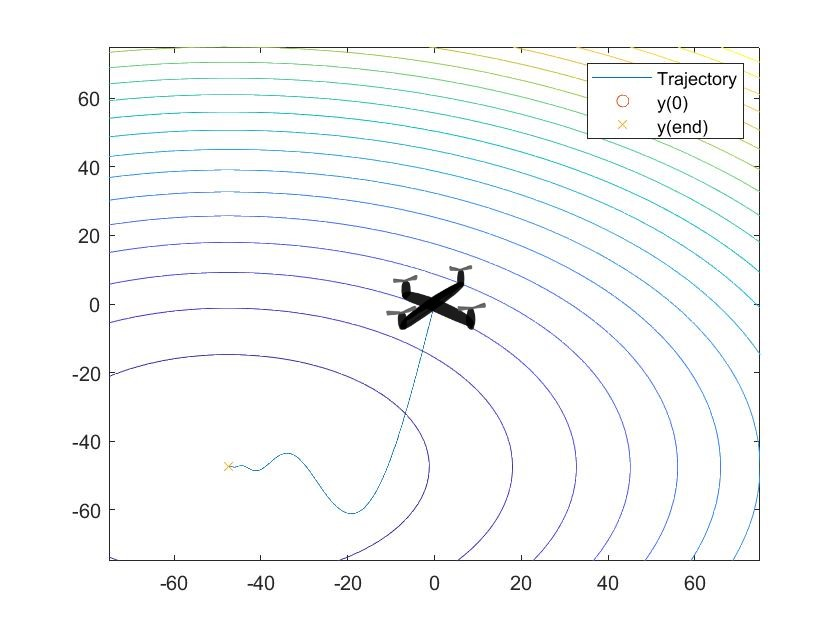
\includegraphics[width=0.9\linewidth,height=0.45\textheight]{figures/single_quad_field.jpg}
			%\caption{Single quadrotor}
			\label{fig:single_quad}
			Single agent
		\end{minipage}%
		\begin{minipage}{0.5\textwidth}
			\centering
			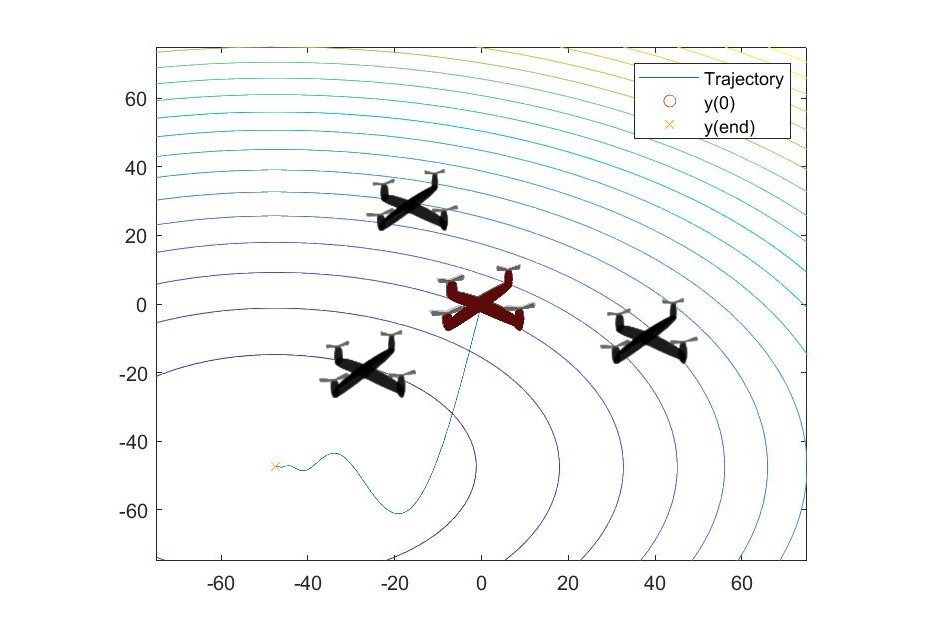
\includegraphics[width=0.9\linewidth,height=0.45\textheight]{figures/multiple_quad_field.jpg}
			%\caption{Multiple quadrotors}
			\label{fig:multiple_quads}
			Multiple agents
		\end{minipage}
	\end{figure}
	\begin{block}{Problem Setting}
		\begin{itemize}		
			\item Field is differentiable and convex
			\item \textit{Noisy} gradients available at some leader agents 
			\item Agent dynamics governed by a quasi-LPV model
		\end{itemize}		
	\end{block}
\end{frame}
%%%%%%%%%%%%%%%%%%%%%%%%%%%%%%%%%%%%%%%%%%%%%%%%%%%%%%%%%%%%%%%%%%%%%
%\begin{frame}{Control Architecture}
%	\begin{figure}[ht]
%		\tikzstyle{block} = [draw, rectangle, 
    minimum height=3em, minimum width=6em]
\tikzstyle{sum} = [draw,  circle, node distance=1cm]
\tikzstyle{input} = [coordinate]
\tikzstyle{output} = [coordinate]
\tikzstyle{pinstyle} = [pin edge={to-,thin,black}]

% The block diagram code is probably more verbose than necessary
%\begin{tikzpicture}[auto, node distance=2cm,>=latex']
%    % We start by placing the blocks
%    \node [input, name=input] {};
%    \node [sum, right of=input] (sum) {};
%    \node [block, right of=sum] (controller) {Controller};
%    \node [block, right of=controller, pin={[pinstyle]above:Disturbances},
%            node distance=3cm] (system) {System};
%    % We draw an edge between the controller and system block to 
%    % calculate the coordinate u. We need it to place the measurement block. 
%    \draw [->] (controller) -- node[name=u] {$u$} (system);
%    \node [output, right of=system] (output) {};
%    \node [block, below of=u] (measurements) {Measurements};
%
%    % Once the nodes are placed, connecting them is easy. 
%    \draw [draw,->] (input) -- node {$r$} (sum);
%    \draw [->] (sum) -- node {$e$} (controller);
%    \draw [->] (system) -- node [name=y] {$y$}(output);
%    \draw [->] (y) |- (measurements);
%    \draw [->] (measurements) -| node[pos=0.99] {$-$} 
%        node [near end] {$y_m$} (sum);
%\end{tikzpicture}

\begin{tikzpicture}[auto, node distance=2cm,>=latex']
% We start by placing the blocks
\node [input, name=input] {};
\node [sum,right of=input](sum_ref) {};
\node [block, right of=input,node distance=3cm](L) {$\mathcal{L}\otimes I_d$};
\node [sum, right of=L,node distance=2cm](sum) {};
\node [block, right of=sum,node distance=2cm,minimum height=2.5em,minimum width=3em](G) {$\left[\begin{array}{c|c}
\hat{A}_G     &  \hat{B}_G\\
\hline
\hat{C}_G     &  \mathbf{0}
\end{array}\right]$};
\node [output, right of=G,node distance=2cm](output) {};
\node [output, right of=G,node distance=1.4cm](outmid) {};
\node [block, above of=G,node distance=2cm](u_psi) {$\begin{bmatrix}0\\ \nabla \psi(y_i)\\ 0\\ \vdots \end{bmatrix}$};
\node [output, below of=L,node distance=2cm](delta) {};


% Once the nodes are placed, connecting them is easy. 
\draw [draw,->] (input) -- node {$-\hat{r}$} (sum_ref);
\draw [draw,->] (sum_ref) -- (L);
\draw [draw,->] (L) -- (sum);
\draw [draw,->] (u_psi) -| (sum);
\draw [draw,->] (sum) -- node {$\hat{u}$} (G);
\draw [draw,->] (G) -- node{$\hat{y}$} (output);
\draw [-] (outmid) |- (delta);
\draw [->] (outmid) |- (u_psi);
\draw [->] (delta) -| (sum_ref);
\end{tikzpicture}
%%		\caption{Control architecture}
%		%\label{fig:control_architecture}	
%	\end{figure}
%\end{frame}
%%%%%%%%%%%%%%%%%%%%%%%%%%%%%%%%%%%%%%%%%%%%%%%%%%%%%%%%%%%%%%%%%%%%%
\begin{frame}{Robust Analysis Problem with Formation Control}
	\begin{overprint}
		\onslide<1>		
		\begin{figure}[!htb]
			\centering
			%		\input{figures/control_arch_rob_control_prob}
			\tikzstyle{block} = [draw, rectangle, 
minimum height=3em, minimum width=6em]
\tikzstyle{sum} = [draw,  circle, node distance=1cm]
\tikzstyle{input} = [coordinate]
\tikzstyle{output} = [coordinate]
\tikzstyle{pinstyle} = [pin edge={to-,thin,black}]

% The block diagram code is probably more verbose than necessary
%\begin{tikzpicture}[auto, node distance=2cm,>=latex']
%    % We start by placing the blocks
%    \node [input, name=input] {};
%    \node [sum, right of=input] (sum) {};
%    \node [block, right of=sum] (controller) {Controller};
%    \node [block, right of=controller, pin={[pinstyle]above:Disturbances},
%            node distance=3cm] (system) {System};
%    % We draw an edge between the controller and system block to 
%    % calculate the coordinate u. We need it to place the measurement block. 
%    \draw [->] (controller) -- node[name=u] {$u$} (system);
%    \node [output, right of=system] (output) {};
%    \node [block, below of=u] (measurements) {Measurements};
%
%    % Once the nodes are placed, connecting them is easy. 
%    \draw [draw,->] (input) -- node {$r$} (sum);
%    \draw [->] (sum) -- node {$e$} (controller);
%    \draw [->] (system) -- node [name=y] {$y$}(output);
%    \draw [->] (y) |- (measurements);
%    \draw [->] (measurements) -| node[pos=0.99] {$-$} 
%        node [near end] {$y_m$} (sum);
%\end{tikzpicture}

\begin{tikzpicture}[auto, node distance=2cm,>=latex']
	% We start by placing the blocks
	\node [input, name=input] {};
	\node [block, right of=input,node distance=2.5cm](Flockcontrol) {$\begin{array}{cc}
			\Dot{q} =& p \\
			\Dot{p} =&-cp-u
		\end{array}$};
	\node [block, right of=Flockcontrol,node distance=4cm,minimum height=2.5em,minimum width=3em](velocityloop) {$\begin{bmatrix}G_{\textnormal{veh}}&&\\&\ddots&\\&&G_{\textnormal{veh}}\end{bmatrix}$};
	\node [output, right of=velocityloop,node distance=3cm](output) {};
	\node [block, below of=Flockcontrol,node distance=3cm, xshift=2cm](delta) {$u=\mathcal{L}_{(d)}y +\begin{bmatrix}
			0\\ .\\ \nabla \psi (y_i)\\.\\ 0
		\end{bmatrix}$};
	%\node[text=red, above left= 5mm and 0.5mm of Flockcontrol] (veh) {$G$};
	%\draw[red, dashed] (veh.east)-|([xshift=-7.8mm]output.west)|-([yshift=-5mm]Flockcontrol.south)-|([xshift=2mm]input.west)|-(veh.west);
	% Once the nodes are placed, connecting them is easy. 
	\draw [draw,->] (input) -- node {$u$} (Flockcontrol);
	\draw [draw,->] (Flockcontrol) -- node {$\begin{bmatrix}q\\p\end{bmatrix}$} (velocityloop);
	\draw [draw,->] (velocityloop) -- node[name=outmid,xshift=3mm] {$y$} (output);
	\draw [-] (outmid) |- (delta);
	\draw [-] (delta) -| (input);
\end{tikzpicture}
		\end{figure}
		%	\onslide<2>
		%	\begin{figure}[!htb]
		%	\centering
		%	%		\input{figures/control_arch_rob_control_prob}
		%	\input{figures/control_arch_rob_control_prob_convex}
		%	\end{figure}
		%	\begin{assumption}
		%		\begin{itemize}
		%			\item $m_{\psi}I\preceq \nabla^2 \psi(y_i) \preceq L_{\psi}I$ (Notation: $\psi \in \mathcal{S}(m_{\psi},L_{\psi})$)
		%			\item Every agent has path to at least 1 informed agent
		%		\end{itemize}
		%	\end{assumption}
		%	$\implies mI\preceq \nabla^2 f(y) \preceq LI$ for suitable $m,L$ (i.e., $f \in \mathcal{S}(m,L)$)
		\onslide<2>
		\begin{figure}[!htb]
			\centering
			%		\input{figures/control_arch_rob_control_prob}
			\tikzstyle{block} = [draw, rectangle, 
minimum height=3em, minimum width=6em]
\tikzstyle{sum} = [draw,  circle, node distance=1cm]
\tikzstyle{input} = [coordinate]
\tikzstyle{output} = [coordinate]
\tikzstyle{pinstyle} = [pin edge={to-,thin,black}]

% The block diagram code is probably more verbose than necessary
%\begin{tikzpicture}[auto, node distance=2cm,>=latex']
%    % We start by placing the blocks
%    \node [input, name=input] {};
%    \node [sum, right of=input] (sum) {};
%    \node [block, right of=sum] (controller) {Controller};
%    \node [block, right of=controller, pin={[pinstyle]above:Disturbances},
%            node distance=3cm] (system) {System};
%    % We draw an edge between the controller and system block to 
%    % calculate the coordinate u. We need it to place the measurement block. 
%    \draw [->] (controller) -- node[name=u] {$u$} (system);
%    \node [output, right of=system] (output) {};
%    \node [block, below of=u] (measurements) {Measurements};
%
%    % Once the nodes are placed, connecting them is easy. 
%    \draw [draw,->] (input) -- node {$r$} (sum);
%    \draw [->] (sum) -- node {$e$} (controller);
%    \draw [->] (system) -- node [name=y] {$y$}(output);
%    \draw [->] (y) |- (measurements);
%    \draw [->] (measurements) -| node[pos=0.99] {$-$} 
%        node [near end] {$y_m$} (sum);
%\end{tikzpicture}

\begin{tikzpicture}[auto, node distance=2cm,>=latex']
	% We start by placing the blocks
	\node [input, name=input] {};
	\node [block, right of=input,node distance=2.5cm](Flockcontrol) {$\begin{array}{cc}
			\Dot{q} =& p \\
			\Dot{p} =&-cp-u
		\end{array}$};
	\node [block, right of=Flockcontrol,node distance=4cm,minimum height=2.5em,minimum width=3em](velocityloop) {$\begin{bmatrix}G_{\textnormal{veh}}&&\\&\ddots&\\&&G_{\textnormal{veh}}\end{bmatrix}$};
	\node [output, right of=velocityloop,node distance=3cm](output) {};
	\node [block, below of=Flockcontrol,node distance=2cm, xshift=2cm](delta) {$u=\nabla f(y)=\nabla \left(y^T\mathcal{L}_{(d)}y + \sum_{i \in \mathcal{V}_l}\psi(y_i)\right)$};
%	\node[text=red, above left= 5mm and 0.5mm of Flockcontrol] (veh) {$G$};
%	\draw[red, dashed] (veh.east)-|([xshift=-7.8mm]output.west)|-([yshift=-5mm]Flockcontrol.south)-|([xshift=2mm]input.west)|-(veh.west);
	% Once the nodes are placed, connecting them is easy. 
	\draw [draw,->] (input) -- node {$u$} (Flockcontrol);
	\draw [draw,->] (Flockcontrol) -- node {$\begin{bmatrix}q\\p\end{bmatrix}$} (velocityloop);
	\draw [draw,->] (velocityloop) -- node[name=outmid,xshift=3mm] {$y$} (output);
	\draw [-] (outmid) |- (delta);
	\draw [-] (delta) -| (input);
\end{tikzpicture}
		\end{figure}
%		\begin{block}{Problem 2}
%			%	\begin{Problem} \label{prob:formation_control}
%			Let $0 \prec m \cdot I\preceq \nabla^2 f(y) \preceq L\cdot I$ (\textcolor{red}{Notation: $f\in \mathcal{S}(m,L)$}), derive sufficient conditions (LMIs) independent of network size under which the state trajectories 
%			\begin{itemize}
%				\item[1)] remain bounded for all $t\geq 0$
%				\item[2)] $\exists \kappa \geq 0$ such that $||y(t)-y_*(t)||\leq \kappa e^{-\alpha t}$ holds for all $t\geq 0$
%			\end{itemize}
%			%	\end{Problem}
%		\end{block}	
		\onslide<3>	\begin{figure}[!htb]
			\centering
			%		\input{figures/control_arch_rob_control_prob}
			\tikzstyle{block} = [draw, rectangle, 
minimum height=3em, minimum width=6em]
\tikzstyle{sum} = [draw,  circle, node distance=1cm]
\tikzstyle{input} = [coordinate]
\tikzstyle{output} = [coordinate]
\tikzstyle{pinstyle} = [pin edge={to-,thin,black}]

% The block diagram code is probably more verbose than necessary
%\begin{tikzpicture}[auto, node distance=2cm,>=latex']
%    % We start by placing the blocks
%    \node [input, name=input] {};
%    \node [sum, right of=input] (sum) {};
%    \node [block, right of=sum] (controller) {Controller};
%    \node [block, right of=controller, pin={[pinstyle]above:Disturbances},
%            node distance=3cm] (system) {System};
%    % We draw an edge between the controller and system block to 
%    % calculate the coordinate u. We need it to place the measurement block. 
%    \draw [->] (controller) -- node[name=u] {$u$} (system);
%    \node [output, right of=system] (output) {};
%    \node [block, below of=u] (measurements) {Measurements};
%
%    % Once the nodes are placed, connecting them is easy. 
%    \draw [draw,->] (input) -- node {$r$} (sum);
%    \draw [->] (sum) -- node {$e$} (controller);
%    \draw [->] (system) -- node [name=y] {$y$}(output);
%    \draw [->] (y) |- (measurements);
%    \draw [->] (measurements) -| node[pos=0.99] {$-$} 
%        node [near end] {$y_m$} (sum);
%\end{tikzpicture}

\begin{tikzpicture}[auto, node distance=2cm,>=latex']
	% We start by placing the blocks
	\node [input, name=input] {};
	\node [block, right of=input,node distance=2.5cm](Flockcontrol) {$\begin{array}{cc}
			\Dot{q} =& p \\
			\Dot{p} =&-cp-u
		\end{array}$};
	\node [block, right of=Flockcontrol,node distance=4cm,minimum height=2.5em,minimum width=3em](velocityloop) {$\begin{bmatrix}G_{\textnormal{veh}}&&\\&\ddots&\\&&G_{\textnormal{veh}}\end{bmatrix}$};
	\node [output, right of=velocityloop,node distance=3cm](output) {};
	\node [block, below of=Flockcontrol,node distance=2cm, xshift=2cm](delta) {$u=(I+\Delta)\nabla f(y)$};
	\node[text=red, above left of= Flockcontrol](veh) {$G$};
	\draw[red, dashed] (veh.east)-|([xshift=-7.8mm]output.west)|-([yshift=-5mm]Flockcontrol.south)-|([xshift=2mm]input.west)|-(veh.west);
	% Once the nodes are placed, connecting them is easy. 
	\draw [draw,->] (input) -- node {$u$} (Flockcontrol);
	\draw [draw,->] (Flockcontrol) -- node {$\begin{bmatrix}q\\p\end{bmatrix}$} (velocityloop);
	\draw [draw,->] (velocityloop) -- node[name=outmid,xshift=3mm] {$y$} (output);
	\draw [-] (outmid) |- (delta);
	\draw [-] (delta) -| (input);
\end{tikzpicture}
		\end{figure}
	\begin{block}{Assume}
		\begin{itemize}
			\item[1] $||\Delta||\leq \delta$
			\item[2] $0 \prec m \cdot I\preceq \nabla^2 f(y) \preceq L\cdot I$ (\textcolor{red}{Notation: $f\in \mathcal{S}(m,L)$}) 
		\end{itemize}
	\end{block}	
%		\begin{block}{Multiplicative Noise}
%			%	\begin{Problem} \label{prob:formation_control}
%			Let $0 \prec m \cdot I\preceq \nabla^2 f(y) \preceq L\cdot I$ (\textcolor{red}{Notation: $f\in \mathcal{S}(m,L)$}), derive sufficient conditions (LMIs) independent of network size under which the state trajectories 
%			\begin{itemize}
%				\item[1)] remain bounded for all $t\geq 0$
%				\item[2)] $\exists \kappa$ such that $||y(t)-y_*(t)||\leq \kappa e^{-\alpha t}$ holds for all $t\geq 0$
%			\end{itemize}
%			%	remain bounded for all $t\geq 0$ and $\exists \kappa \geq 0$ such that $||y(t)-y_*(t)||\leq \kappa e^{-\alpha t}$ holds for all $t\geq 0$.
%			%	\end{Problem}
%		\end{block}
	\end{overprint}
\end{frame}
%%%%%%%%%%%%%%%%%%%%%%%%%%%%%%%%%%%%%%%%%%%%%%%%%%%%%%%%%%%%%%%%%%%%
\begin{frame}{Control Architecture: Multiple agents}
	\begin{equation*} %\label{eq:sys_dyn_G}
		\begin{split}
			\Dot{{\eta}}(t)&=\hat{A}_G(\rho(t)){\eta}(t) + \hat{B}_G(\rho(t)) {u}(t), \quad \quad {\eta}(0)={\eta}_{0},\\
			{y}(t)&=\hat{C}_G(\rho(t)) {\eta}(t). \\
		\end{split}
	\end{equation*}
	where, notation $\hat{X}=I_N \otimes X$ and ${x}=[x_1^T,\hdots,x_N^T]^T$ is used.
	%	\pause
	\begin{block}{Formation control law with gradient-based forcing term}
		\begin{equation}\label{eq:control_law}
			{u}=\mathcal{L}_{(d)}({y}-{r})+\begin{bmatrix}u_{\psi_1}\\ \vdots \\u_{\psi_N}\end{bmatrix}.
		\end{equation}
		
		\begin{equation}\label{eq:forcing_term}
			\begin{split}
				u_{\psi_i}(t)&=
				\begin{cases}
					\nabla \psi(y_i), & \text{if}\ i\in \mathcal{V}_l, \\
					0, & \text{otherwise}.
				\end{cases}
			\end{split}
		\end{equation}
	\end{block}
\end{frame}
%%%%%%%%%%%%%%%%%%%%%%%%%%%%%%%%%%%%%%%%%%%%%%%%%%%%%%%%%%%%%%%%%%%%%
\begin{frame}{qLPV modeling}
\begin{block}{Assume}
There exists a function $g:\mathbb{R}^{n_{\eta}}\rightarrow\mathbb{R}^{n_{\rho}}$ such that $\rho(t)=g(\eta(t))\quad t\in[0,\infty)$ and there exists $c\geq 0$ such that 
\begin{equation*}
	\mathcal{B}(\eta_*,c)=\left\{ \eta:||\eta-\eta_*|| \leq c \right\} \subset \{\eta\in \mathbb{R}^{n_{\eta}}:g(\eta)\in \mathcal{P}\}=:\mathcal{P}^{-1}_g
\end{equation*}
\end{block}
\pause 
\begin{block}{Examples with $\eta=[x_1\quad x_2]^T$, $g:\mathbb{R}^2\rightarrow \mathbb{R}$, $\mathcal{P}=[-0.5,0.5]$}
\end{block}
%\begin{overprint}
%\onslide<+>
%1: $\rho=x_1$
%\onslide<+>
%2: $\rho=x_1+\textnormal{sign}(x_2)$
%\end{overprint}
%\vspace{2cm}
\begin{figure}
	
\begin{minipage}{.5\textwidth}
	\centering
	$\rho=x_1$
	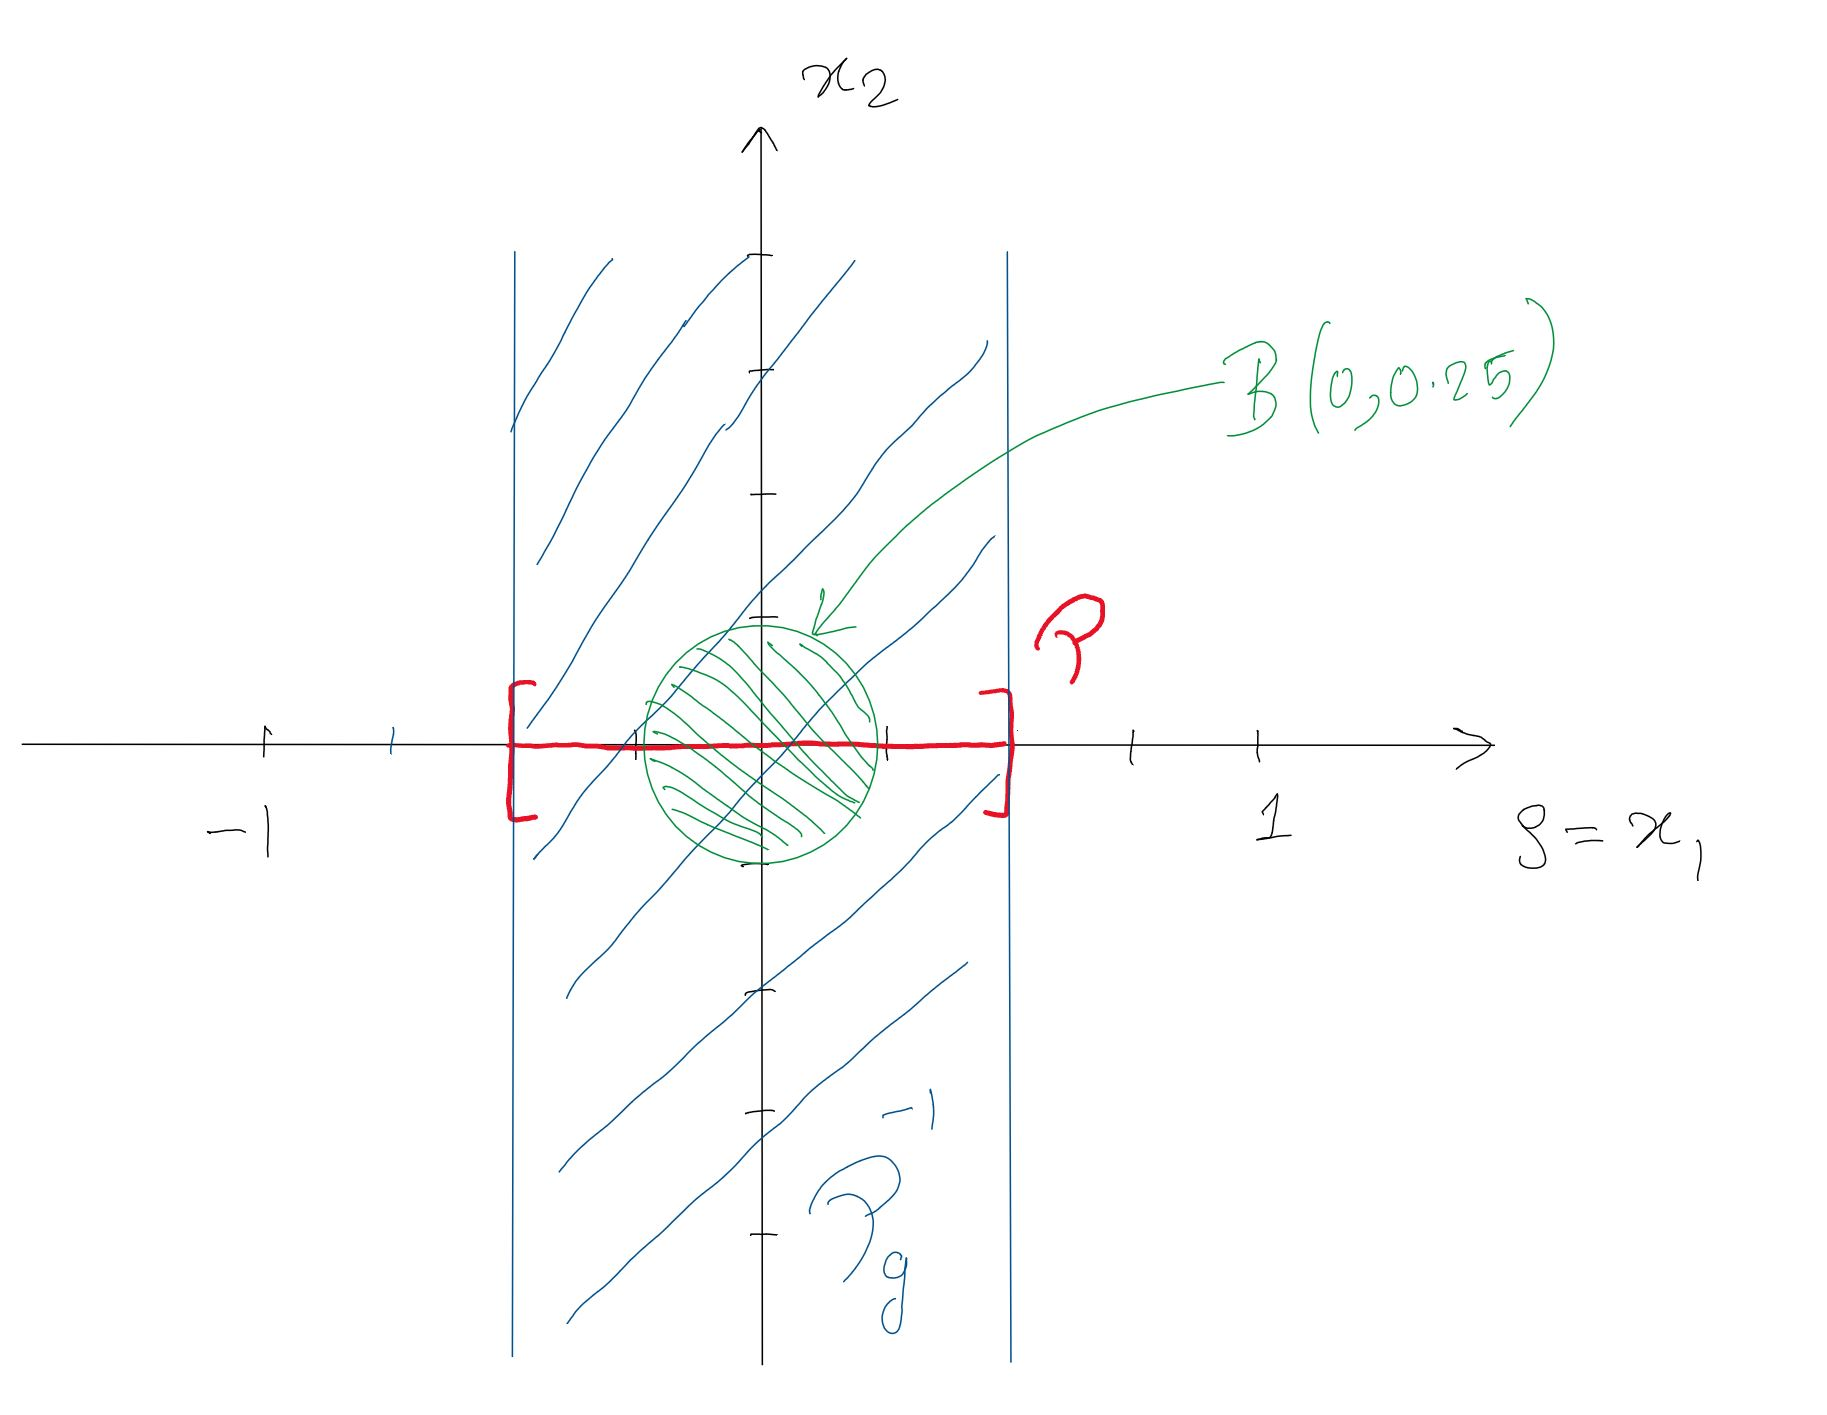
\includegraphics[width=0.9\linewidth,height=0.43\textheight]{figures/sched_para_map_valid.jpg}
	%\caption{Single quadrotor}
\end{minipage}%
\begin{minipage}{0.5\textwidth}
	\centering
	$\rho=x_1+\textnormal{sign}(x_2)$
	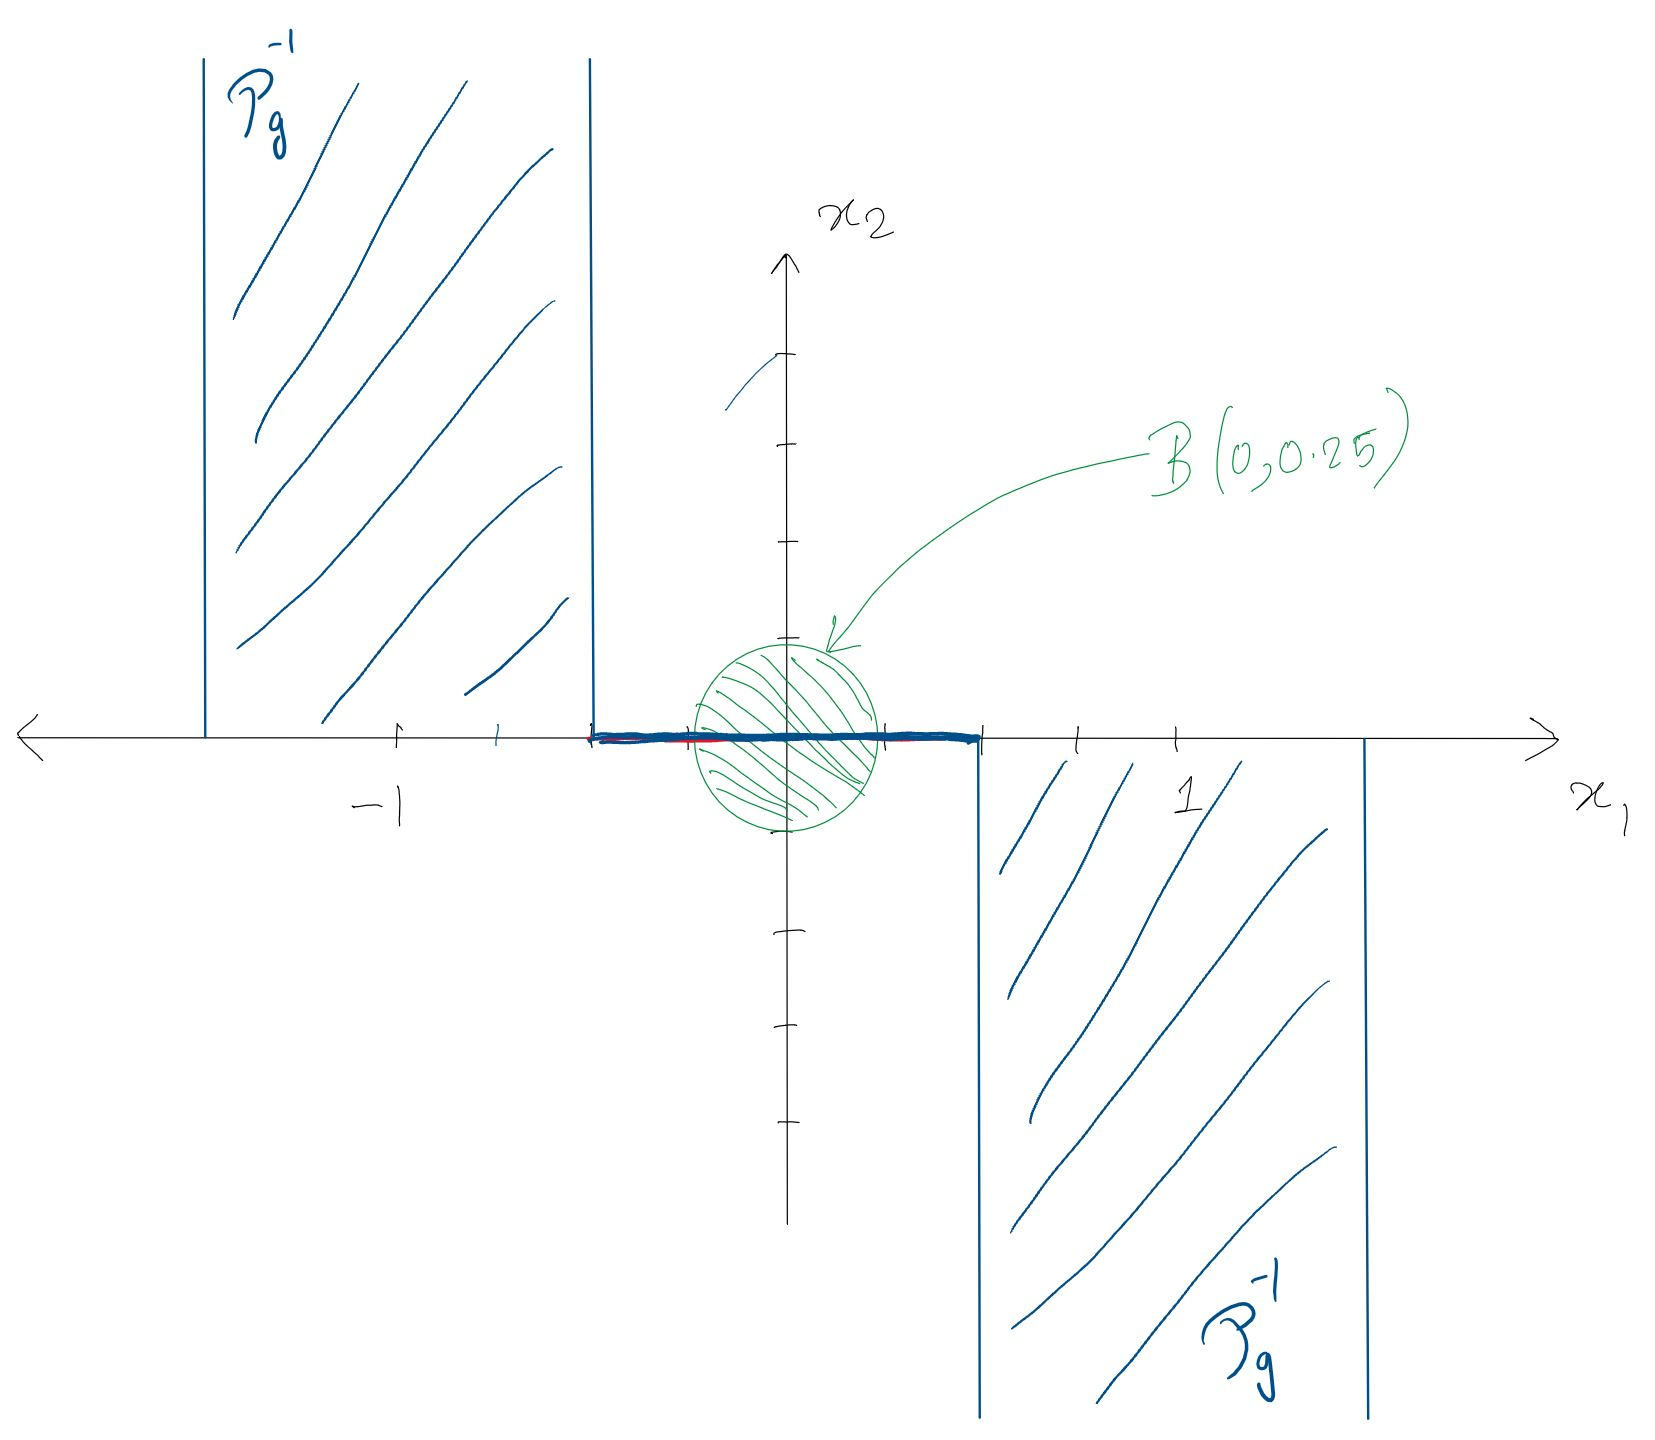
\includegraphics[width=0.9\linewidth,height=0.43\textheight]{figures/sched_para_map_invalid.jpg}
	%\caption{Multiple quadrotors}
\end{minipage}
\end{figure}
\end{frame}
%%%%%%%%%%%%%%%%%%%%%%%%%%%%%%%%%%%%%%%%%%%%%%%%%%%%%%%%%%%%%%%%%%%%%
\begin{frame}{Main Result}
	\begin{block}{Theorem}	
			If there exist $\mathcal{X}_0\succ 0,P \in \mathbb{P}$, $\lambda \geq 0$ such that 
			\begin{align}\label{eq:perf_LMI_noise_single}
				%		\begin{split}
				&\begin{bmatrix}
					\mathcal{A}_0(\tilde{\rho})^T\mathcal{X}_0+\mathcal{X}\mathcal{A}_0(\tilde{\rho})+2\alpha \mathcal{X}_0  & (*) \\
					\mathcal{B}_0(\tilde{\rho})^T\mathcal{X}_0    & \mathbf{0}
				\end{bmatrix} \nonumber \\
				&\hspace{0.1cm}+			
				(*)
				\begin{bmatrix}
					P \otimes I_d &\\&\lambda (M \otimes I_d)
				\end{bmatrix}
				\begin{bmatrix}
					\mathcal{C}_{10}(\tilde{\rho}) & \mathcal{D}_{10}\\
					\mathcal{C}_{20} &\mathcal{D}_{20}\\
				\end{bmatrix}
				\preceq 
				0,
				%		\end{split}
			\end{align}
		holds for all $\tilde{\rho} \in \mathcal{P}$,
			then for all initial conditions $\eta_0$ such that $||\eta_0-\eta_*||< \frac{c}{\sqrt{\textnormal{cond}(\mathcal{X})}}$, the trajectories converge to the equilibrium exponentially at rate $\alpha$.
	\end{block}

\end{frame}
%%%%%%%%%%%%%%%%%%%%%%%%%%%%%%%%%%%%%%%%%%%%%%%%%%%%%%%%%%%%%%%%%%%%%
\begin{frame}{Numerical results for a single LTI quadrotor}
	\begin{figure}[ht]
		\tikzstyle{block} = [draw, rectangle, 
    minimum height=3em, minimum width=6em]
\tikzstyle{sum} = [draw,  circle, node distance=1cm]
\tikzstyle{input} = [coordinate]
\tikzstyle{output} = [coordinate]
\tikzstyle{pinstyle} = [pin edge={to-,thin,black}]

% The block diagram code is probably more verbose than necessary
%\begin{tikzpicture}[auto, node distance=2cm,>=latex']
%    % We start by placing the blocks
%    \node [input, name=input] {};
%    \node [sum, right of=input] (sum) {};
%    \node [block, right of=sum] (controller) {Controller};
%    \node [block, right of=controller, pin={[pinstyle]above:Disturbances},
%            node distance=3cm] (system) {System};
%    % We draw an edge between the controller and system block to 
%    % calculate the coordinate u. We need it to place the measurement block. 
%    \draw [->] (controller) -- node[name=u] {$u$} (system);
%    \node [output, right of=system] (output) {};
%    \node [block, below of=u] (measurements) {Measurements};
%
%    % Once the nodes are placed, connecting them is easy. 
%    \draw [draw,->] (input) -- node {$r$} (sum);
%    \draw [->] (sum) -- node {$e$} (controller);
%    \draw [->] (system) -- node [name=y] {$y$}(output);
%    \draw [->] (y) |- (measurements);
%    \draw [->] (measurements) -| node[pos=0.99] {$-$} 
%        node [near end] {$y_m$} (sum);
%\end{tikzpicture}

\begin{tikzpicture}[auto, node distance=2cm,>=latex']
% We start by placing the blocks
\node [input, name=input] {};
\node [block, right of=input,node distance=3cm](Flockcontrol) {$\begin{array}{cc}
   \Dot{q} =& p \\
   \Dot{p} =&-k_d p-k_p u
\end{array}$};
\node [block, right of=Flockcontrol,node distance=4cm,minimum height=2.5em,minimum width=3em](velocityloop) {$\left[\begin{array}{c|c}
A     &  B\\
\hline
C     &  \mathbf{0}
\end{array}\right]$};
\node [output, right of=velocityloop,node distance=1.4cm](output) {};
\node [block, below of=Flockcontrol,node distance=2cm](delta) {$u=\nabla f(y)$};
\node[text=red, above of = Flockcontrol,xshift=-2cm,yshift=-0.5cm] (veh) {$G$};
\draw[red, dashed] (veh.east)-|([xshift=-3.8mm]output.west)|-([yshift=-3mm]Flockcontrol.south)-|([xshift=2mm]input.west)|-(veh.west);
% Once the nodes are placed, connecting them is easy. 
\draw [draw,->] (input) -- node {$u$} (Flockcontrol);
\draw [draw,->] (Flockcontrol) -- node {$\begin{bmatrix}q\\p\end{bmatrix}$} (velocityloop);
\draw [draw,->] (velocityloop) -- node[name=outmid] {$y$} (output);
\draw [->] (outmid) |- (delta);
\draw [-] (delta) -| (input);
\end{tikzpicture}
		%\caption{Control architecture}	
	\end{figure}
	\begin{block}{Setup}
		\begin{itemize}
			\item Linearized quadrotor model + LQR local controller
			\item $||\Delta||\leq \delta$
		\end{itemize}
	\end{block}	
\end{frame}
\begin{frame}{Designing $k_d$ for largest convergence rate estimate $\alpha$}
	\begin{figure}[h!]
		%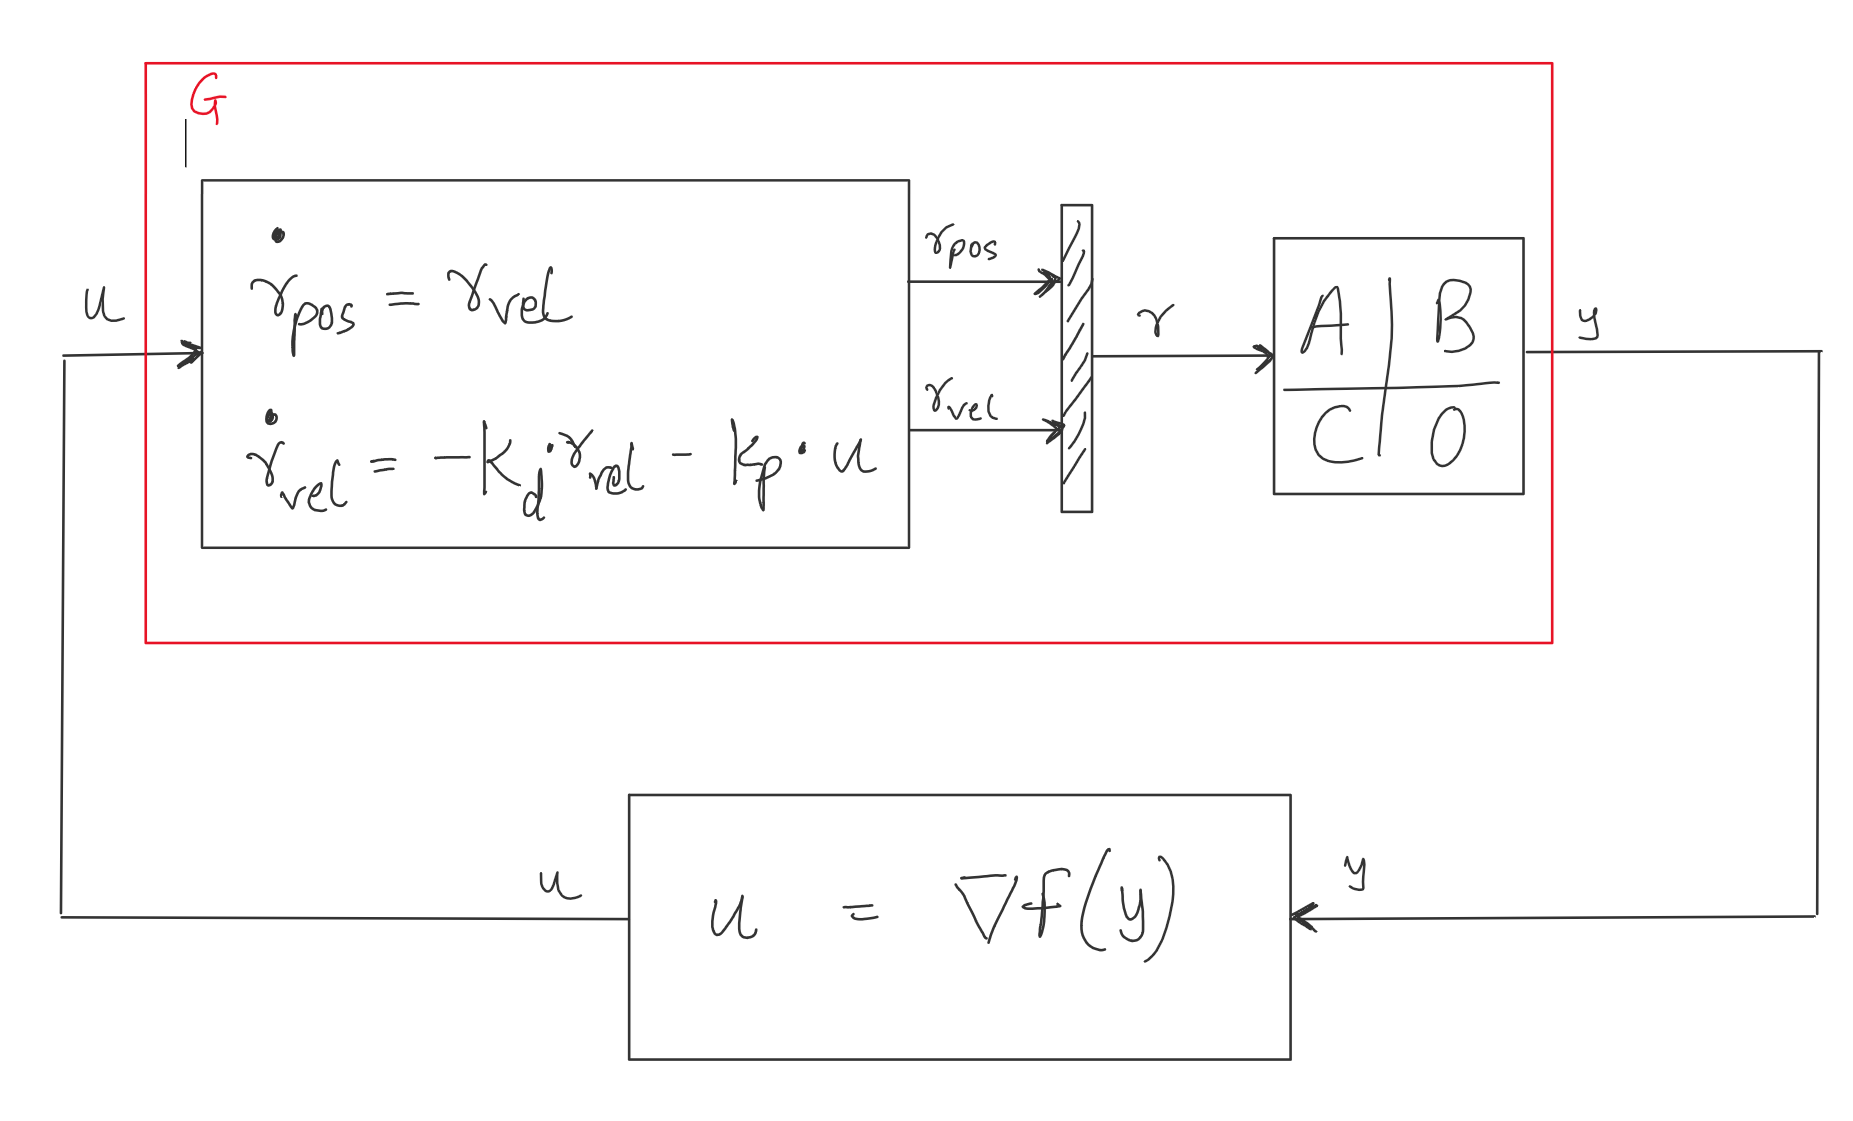
\includegraphics[width=8cm]{figures/Figure_IQC_paper.PNG}
		\centering
		% This file was created by matlab2tikz.
%
%The latest updates can be retrieved from
%  http://www.mathworks.com/matlabcentral/fileexchange/22022-matlab2tikz-matlab2tikz
%where you can also make suggestions and rate matlab2tikz.
%
\definecolor{mycolor1}{rgb}{0.09091,0.00000,0.90909}%
%
\begin{tikzpicture}

\begin{axis}[%
width=2.521in,
height=2.366in,
at={(0.758in,0.481in)},
scale only axis,
xmin=5,
xmax=30,
xlabel style={font=\color{white!15!black}},
xlabel={$k_d$},
ymin=0,
ymax=0.2,
ylabel style={font=\color{white!15!black}},
ylabel={$\alpha$},
axis background/.style={fill=white},
title style={font=\bfseries},
title={},
legend style={legend cell align=left, align=left, draw=white!15!black}
]
\addplot [color=red!0!mycolor1, dashed, line width=1.0pt]
  table[row sep=crcr]{%
1	-1\\
1.5	-1\\
2	-1\\
2.5	-1\\
3	-1\\
3.5	-1\\
4	-1\\
4.5	-1\\
5	-1\\
5.5	-1\\
6	0.001220703125\\
6.5	0.0311279296875\\
7	0.0579833984375\\
7.5	0.081787109375\\
8	0.103759765625\\
8.5	0.123291015625\\
9	0.140380859375\\
9.5	0.130615234375\\
10	0.1226806640625\\
10.5	0.1153564453125\\
11	0.108642578125\\
11.5	0.1025390625\\
12	0.09765625\\
12.5	0.0927734375\\
13	0.0885009765625\\
13.5	0.0848388671875\\
14	0.0811767578125\\
16	0.069580078125\\
18	0.06103515625\\
20	0.0543212890625\\
22	0.048828125\\
24	0.0445556640625\\
26	0.0408935546875\\
28	0.037841796875\\
};
\addlegendentry{$\delta=0$}
%\addplot [color=mycolor1, line width=1.0pt, forget plot]
%  table[row sep=crcr]{%
%1	-1\\
%1.5	-1\\
%2	-1\\
%2.5	-1\\
%3	-1\\
%3.5	-1\\
%4	-1\\
%4.5	-1\\
%5	-1\\
%5.5	-1\\
%6	0.001220703125\\
%6.5	0.0311279296875\\
%7	0.0579833984375\\
%7.5	0.081787109375\\
%8	0.103759765625\\
%8.5	0.123291015625\\
%9	0.1385498046875\\
%9.5	0.130615234375\\
%10	0.1226806640625\\
%10.5	0.1153564453125\\
%11	0.108642578125\\
%11.5	0.1025390625\\
%12	0.09765625\\
%12.5	0.0872802734375\\
%13	0.0885009765625\\
%13.5	0.0848388671875\\
%14	0.0811767578125\\
%14.5	0.078125\\
%15	0.0750732421875\\
%15.5	0.072021484375\\
%16	0.069580078125\\
%16.5	0.067138671875\\
%17	0.0653076171875\\
%17.5	0.0628662109375\\
%18	0.06103515625\\
%18.5	0.0592041015625\\
%19	0.057373046875\\
%19.5	0.0555419921875\\
%20	0.0543212890625\\
%20.5	0.0531005859375\\
%21	0.05126953125\\
%21.5	0.050048828125\\
%22	0.048828125\\
%22.5	0.047607421875\\
%23	0.04638671875\\
%23.5	0.045166015625\\
%24	0.0445556640625\\
%24.5	0.0433349609375\\
%25	0.042724609375\\
%25.5	0.04150390625\\
%26	0.0408935546875\\
%26.5	0.0396728515625\\
%27	0.0390625\\
%27.5	0.0384521484375\\
%28	0.037841796875\\
%};

\addplot [color=red!10!mycolor1, line width=1.0pt]
  table[row sep=crcr]{%
1	-1\\
1.5	-1\\
2	-1\\
2.5	-1\\
3	-1\\
3.5	-1\\
4	-1\\
4.5	-1\\
5	-1\\
5.5	-1\\
6	-1\\
6.5	-1\\
7	0.006103515625\\
7.5	0.030517578125\\
8	0.052490234375\\
8.5	0.0726318359375\\
9	0.0909423828125\\
9.5	0.1080322265625\\
10	0.107421875\\
10.5	0.101318359375\\
11	0.09521484375\\
11.5	0.09033203125\\
12	0.0860595703125\\
12.5	0.081787109375\\
13	0.078125\\
13.5	0.0750732421875\\
14	0.072021484375\\
14.5	0.0689697265625\\
15	0.0665283203125\\
15.5	0.0640869140625\\
16	0.0616455078125\\
16.5	0.059814453125\\
17	0.0579833984375\\
17.5	0.05615234375\\
18	0.0543212890625\\
18.5	0.052490234375\\
19	0.05126953125\\
19.5	0.0494384765625\\
20	0.0482177734375\\
20.5	0.0469970703125\\
21	0.0457763671875\\
21.5	0.0445556640625\\
22	0.0433349609375\\
22.5	0.042724609375\\
23	0.04150390625\\
23.5	0.040283203125\\
24	0.0396728515625\\
24.5	0.0390625\\
25	0.037841796875\\
25.5	0.0372314453125\\
26	0.03662109375\\
26.5	0.035400390625\\
27	0.0347900390625\\
27.5	0.0341796875\\
28	0.0335693359375\\
};
\addlegendentry{$\delta=0.1$}
\addplot [color=red!20!mycolor1, line width=1.0pt, forget plot]
  table[row sep=crcr]{%
1	-1\\
1.5	-1\\
2	-1\\
2.5	-1\\
3	-1\\
3.5	-1\\
4	-1\\
4.5	-1\\
5	-1\\
5.5	-1\\
6	-1\\
6.5	-1\\
7	-1\\
7.5	-1\\
8	0.0048828125\\
8.5	0.0250244140625\\
9	0.0439453125\\
9.5	0.06103515625\\
10	0.0762939453125\\
10.5	0.0872802734375\\
11	0.0830078125\\
11.5	0.0787353515625\\
12	0.0750732421875\\
12.5	0.0714111328125\\
13	0.068359375\\
13.5	0.06591796875\\
14	0.0628662109375\\
14.5	0.0604248046875\\
15	0.05859375\\
15.5	0.05615234375\\
16	0.0543212890625\\
16.5	0.052490234375\\
17	0.0506591796875\\
17.5	0.0494384765625\\
18	0.047607421875\\
18.5	0.04638671875\\
19	0.045166015625\\
19.5	0.0439453125\\
20	0.042724609375\\
20.5	0.04150390625\\
21	0.040283203125\\
21.5	0.0390625\\
22	0.0384521484375\\
22.5	0.0372314453125\\
23	0.03662109375\\
23.5	0.0360107421875\\
24	0.0347900390625\\
24.5	0.0341796875\\
25	0.0335693359375\\
25.5	0.032958984375\\
26	0.0323486328125\\
26.5	0.03173828125\\
27	0.030517578125\\
27.5	0.030517578125\\
28	0.0299072265625\\
};
\addplot [color=red!30!mycolor1, line width=1.0pt, forget plot]
  table[row sep=crcr]{%
1	-1\\
1.5	-1\\
2	-1\\
2.5	-1\\
3	-1\\
3.5	-1\\
4	-1\\
4.5	-1\\
5	-1\\
5.5	-1\\
6	-1\\
6.5	-1\\
7	-1\\
7.5	-1\\
8	-1\\
8.5	-1\\
9	-1\\
9.5	0.015869140625\\
10	0.0323486328125\\
10.5	0.0469970703125\\
11	0.0604248046875\\
11.5	0.0677490234375\\
12	0.064697265625\\
12.5	0.0616455078125\\
13	0.0592041015625\\
13.5	0.05615234375\\
14	0.0543212890625\\
14.5	0.052490234375\\
15	0.050048828125\\
15.5	0.048828125\\
16	0.0469970703125\\
16.5	0.045166015625\\
17	0.0439453125\\
17.5	0.042724609375\\
18	0.04150390625\\
18.5	0.040283203125\\
19	0.0390625\\
19.5	0.037841796875\\
20	0.03662109375\\
20.5	0.0360107421875\\
21	0.0347900390625\\
21.5	0.0341796875\\
22	0.032958984375\\
22.5	0.0323486328125\\
23	0.03173828125\\
23.5	0.0311279296875\\
24	0.030517578125\\
24.5	0.0299072265625\\
25	0.029296875\\
25.5	0.0286865234375\\
26	0.028076171875\\
26.5	0.0274658203125\\
27	0.02685546875\\
27.5	0.0262451171875\\
28	0.025634765625\\
};
\addplot [color=red!40!mycolor1, line width=1.0pt, forget plot]
  table[row sep=crcr]{%
1	-1\\
1.5	-1\\
2	-1\\
2.5	-1\\
3	-1\\
3.5	-1\\
4	-1\\
4.5	-1\\
5	-1\\
5.5	-1\\
6	-1\\
6.5	-1\\
7	-1\\
7.5	-1\\
8	-1\\
8.5	-1\\
9	-1\\
9.5	-1\\
10	-1\\
10.5	0.0048828125\\
11	0.018310546875\\
11.5	0.0311279296875\\
12	0.0433349609375\\
12.5	0.0518798828125\\
13	0.0494384765625\\
13.5	0.047607421875\\
14	0.0457763671875\\
14.5	0.0439453125\\
15	0.042724609375\\
15.5	0.0408935546875\\
16	0.0396728515625\\
16.5	0.0384521484375\\
17	0.0372314453125\\
17.5	0.0360107421875\\
18	0.0347900390625\\
18.5	0.0341796875\\
19	0.032958984375\\
19.5	0.0323486328125\\
20	0.0311279296875\\
20.5	0.0299072265625\\
21	0.0299072265625\\
21.5	0.0286865234375\\
22	0.028076171875\\
22.5	0.0274658203125\\
23	0.02685546875\\
23.5	0.0262451171875\\
24	0.025634765625\\
24.5	0.0250244140625\\
25	0.0244140625\\
25.5	0.0244140625\\
26	0.0238037109375\\
26.5	0.023193359375\\
27	0.0225830078125\\
27.5	0.0225830078125\\
28	0.02197265625\\
};
\addplot [color=red!50!mycolor1, line width=1.0pt]
  table[row sep=crcr]{%
1	-1\\
1.5	-1\\
2	-1\\
2.5	-1\\
3	-1\\
3.5	-1\\
4	-1\\
4.5	-1\\
5	-1\\
5.5	-1\\
6	-1\\
6.5	-1\\
7	-1\\
7.5	-1\\
8	-1\\
8.5	-1\\
9	-1\\
9.5	-1\\
10	-1\\
10.5	-1\\
11	-1\\
11.5	-1\\
12	0.003662109375\\
12.5	0.0152587890625\\
13	0.025634765625\\
13.5	0.035400390625\\
14	0.037841796875\\
14.5	0.0360107421875\\
15	0.0347900390625\\
15.5	0.0335693359375\\
16	0.0323486328125\\
16.5	0.03173828125\\
17	0.030517578125\\
17.5	0.0299072265625\\
18	0.0286865234375\\
18.5	0.028076171875\\
19	0.0274658203125\\
19.5	0.0262451171875\\
20	0.025634765625\\
20.5	0.0250244140625\\
21	0.0244140625\\
21.5	0.0238037109375\\
22	0.023193359375\\
22.5	0.0225830078125\\
23	0.02197265625\\
23.5	0.02197265625\\
24	0.0213623046875\\
24.5	0.020751953125\\
25	0.0201416015625\\
25.5	0.0201416015625\\
26	0.01953125\\
26.5	0.0189208984375\\
27	0.0189208984375\\
27.5	0.018310546875\\
28	0.018310546875\\
};
\addlegendentry{$\delta=0.5$}
\addplot [color=red!60!mycolor1, line width=1.0pt, forget plot]
  table[row sep=crcr]{%
1	-1\\
1.5	-1\\
2	-1\\
2.5	-1\\
3	-1\\
3.5	-1\\
4	-1\\
4.5	-1\\
5	-1\\
5.5	-1\\
6	-1\\
6.5	-1\\
7	-1\\
7.5	-1\\
8	-1\\
8.5	-1\\
9	-1\\
9.5	-1\\
10	-1\\
10.5	-1\\
11	-1\\
11.5	-1\\
12	-1\\
12.5	-1\\
13	-1\\
13.5	-1\\
14	0.00732421875\\
14.5	0.0164794921875\\
15	0.0244140625\\
15.5	0.02685546875\\
16	0.025634765625\\
16.5	0.0250244140625\\
17	0.0244140625\\
17.5	0.023193359375\\
18	0.0225830078125\\
18.5	0.02197265625\\
19	0.0213623046875\\
19.5	0.020751953125\\
20	0.0201416015625\\
20.5	0.01953125\\
21	0.01953125\\
21.5	0.0189208984375\\
22	0.018310546875\\
22.5	0.0177001953125\\
23	0.0177001953125\\
23.5	0.01708984375\\
24	0.01708984375\\
24.5	0.0164794921875\\
25	0.015869140625\\
25.5	0.015869140625\\
26	0.0152587890625\\
26.5	0.0152587890625\\
27	0.0146484375\\
27.5	0.0146484375\\
28	0.0140380859375\\
};
\addplot [color=red!70!mycolor1, line width=1.0pt, forget plot]
  table[row sep=crcr]{%
1	-1\\
1.5	-1\\
2	-1\\
2.5	-1\\
3	-1\\
3.5	-1\\
4	-1\\
4.5	-1\\
5	-1\\
5.5	-1\\
6	-1\\
6.5	-1\\
7	-1\\
7.5	-1\\
8	-1\\
8.5	-1\\
9	-1\\
9.5	-1\\
10	-1\\
10.5	-1\\
11	-1\\
11.5	-1\\
12	-1\\
12.5	-1\\
13	-1\\
13.5	-1\\
14	-1\\
14.5	-1\\
15	-1\\
15.5	-1\\
16	0.0042724609375\\
16.5	0.010986328125\\
17	0.0177001953125\\
17.5	0.01708984375\\
18	0.01708984375\\
18.5	0.0164794921875\\
19	0.015869140625\\
19.5	0.0152587890625\\
20	0.0152587890625\\
20.5	0.0146484375\\
21	0.0140380859375\\
21.5	0.0140380859375\\
22	0.013427734375\\
22.5	0.013427734375\\
23	0.0128173828125\\
23.5	0.0128173828125\\
24	0.01220703125\\
24.5	0.01220703125\\
25	0.01220703125\\
25.5	0.0115966796875\\
26	0.0115966796875\\
26.5	0.010986328125\\
27	0.010986328125\\
27.5	0.010986328125\\
28	0.0103759765625\\
};
\addplot [color=red!80!mycolor1, line width=1.0pt, forget plot]
  table[row sep=crcr]{%
1	-1\\
1.5	-1\\
2	-1\\
2.5	-1\\
3	-1\\
3.5	-1\\
4	-1\\
4.5	-1\\
5	-1\\
5.5	-1\\
6	-1\\
6.5	-1\\
7	-1\\
7.5	-1\\
8	-1\\
8.5	-1\\
9	-1\\
9.5	-1\\
10	-1\\
10.5	-1\\
11	-1\\
11.5	-1\\
12	-1\\
12.5	-1\\
13	-1\\
13.5	-1\\
14	-1\\
14.5	-1\\
15	-1\\
15.5	-1\\
16	-1\\
16.5	-1\\
17	-1\\
17.5	-1\\
18	-1\\
18.5	0.001220703125\\
19	0.0067138671875\\
19.5	0.0103759765625\\
20	0.009765625\\
20.5	0.009765625\\
21	0.0091552734375\\
21.5	0.0091552734375\\
22	0.0091552734375\\
22.5	0.008544921875\\
23	0.008544921875\\
23.5	0.008544921875\\
24	0.0079345703125\\
24.5	0.0079345703125\\
25	0.0079345703125\\
25.5	0.00732421875\\
26	0.00732421875\\
26.5	0.00732421875\\
27	0.00732421875\\
27.5	0.00732421875\\
28	0.0067138671875\\
};
\addplot [color=red!90!mycolor1, line width=1.0pt]
  table[row sep=crcr]{%
1	-1\\
1.5	-1\\
2	-1\\
2.5	-1\\
3	-1\\
3.5	-1\\
4	-1\\
4.5	-1\\
5	-1\\
5.5	-1\\
6	-1\\
6.5	-1\\
7	-1\\
7.5	-1\\
8	-1\\
8.5	-1\\
9	-1\\
9.5	-1\\
10	-1\\
10.5	-1\\
11	-1\\
11.5	-1\\
12	-1\\
12.5	-1\\
13	-1\\
13.5	-1\\
14	-1\\
14.5	-1\\
15	-1\\
15.5	-1\\
16	-1\\
16.5	-1\\
17	-1\\
17.5	-1\\
18	-1\\
18.5	-1\\
19	-1\\
19.5	-1\\
20	-1\\
20.5	-1\\
21	-1\\
21.5	-1\\
22	-1\\
22.5	0.00244140625\\
23	0.0042724609375\\
23.5	0.003662109375\\
24	0.003662109375\\
24.5	0.003662109375\\
25	0.003662109375\\
25.5	0.003662109375\\
26	0.003662109375\\
26.5	0.0030517578125\\
27	0.0030517578125\\
27.5	0.0030517578125\\
28	0.0030517578125\\
};
\addlegendentry{$\delta=0.9$}

%\addplot [color=red, line width=1.0pt, forget plot]
%  table[row sep=crcr]{%
%1	-1\\
%1.5	-1\\
%2	-1\\
%2.5	-1\\
%3	-1\\
%3.5	-1\\
%4	-1\\
%4.5	-1\\
%5	-1\\
%5.5	-1\\
%6	-1\\
%6.5	-1\\
%7	-1\\
%7.5	-1\\
%8	-1\\
%8.5	-1\\
%9	-1\\
%9.5	-1\\
%10	-1\\
%10.5	-1\\
%11	-1\\
%11.5	-1\\
%12	-1\\
%12.5	-1\\
%13	-1\\
%13.5	-1\\
%14	-1\\
%14.5	-1\\
%15	-1\\
%15.5	-1\\
%16	-1\\
%16.5	-1\\
%17	-1\\
%17.5	-1\\
%18	-1\\
%18.5	-1\\
%19	-1\\
%19.5	-1\\
%20	-1\\
%20.5	-1\\
%21	-1\\
%21.5	-1\\
%22	-1\\
%22.5	-1\\
%23	-1\\
%23.5	-1\\
%24	-1\\
%24.5	-1\\
%25	-1\\
%25.5	-1\\
%26	-1\\
%26.5	-1\\
%27	-1\\
%27.5	-1\\
%28	-1\\
%};
\end{axis}

% \begin{axis}[%
% width=5.833in,
% height=4.375in,
% at={(0in,0in)},
% scale only axis,
% xmin=0,
% xmax=1,
% ymin=0,
% ymax=1,
% axis line style={draw=none},
% ticks=none,
% axis x line*=bottom,
% axis y line*=left
% ]
% \end{axis}
\end{tikzpicture}%
%		\caption{Performance estimates for quadrotor dynamics provided by first order ZF multipliers for $\psi \in \mathcal{S}(1,10)$ and varying $k_d$ with different bound $\delta \in \{0.1,0.2\cdots,0.9\}$ on the multiplicative noise (see Assumption \ref{assum:noise}).}
		\label{fig:quadrotor_optimal_kd_ZF_noisy}
	\end{figure}
\end{frame}
%%%%%%%%%%%%%%%%%%%%%%%%%%%%%%%%%%%%%%%%%%%%%%%%%%%%%%%%%%%%%%%%%%%%%
\begin{frame}{Conservatism estimation by searching for examples}
	\begin{figure}[h!]
		%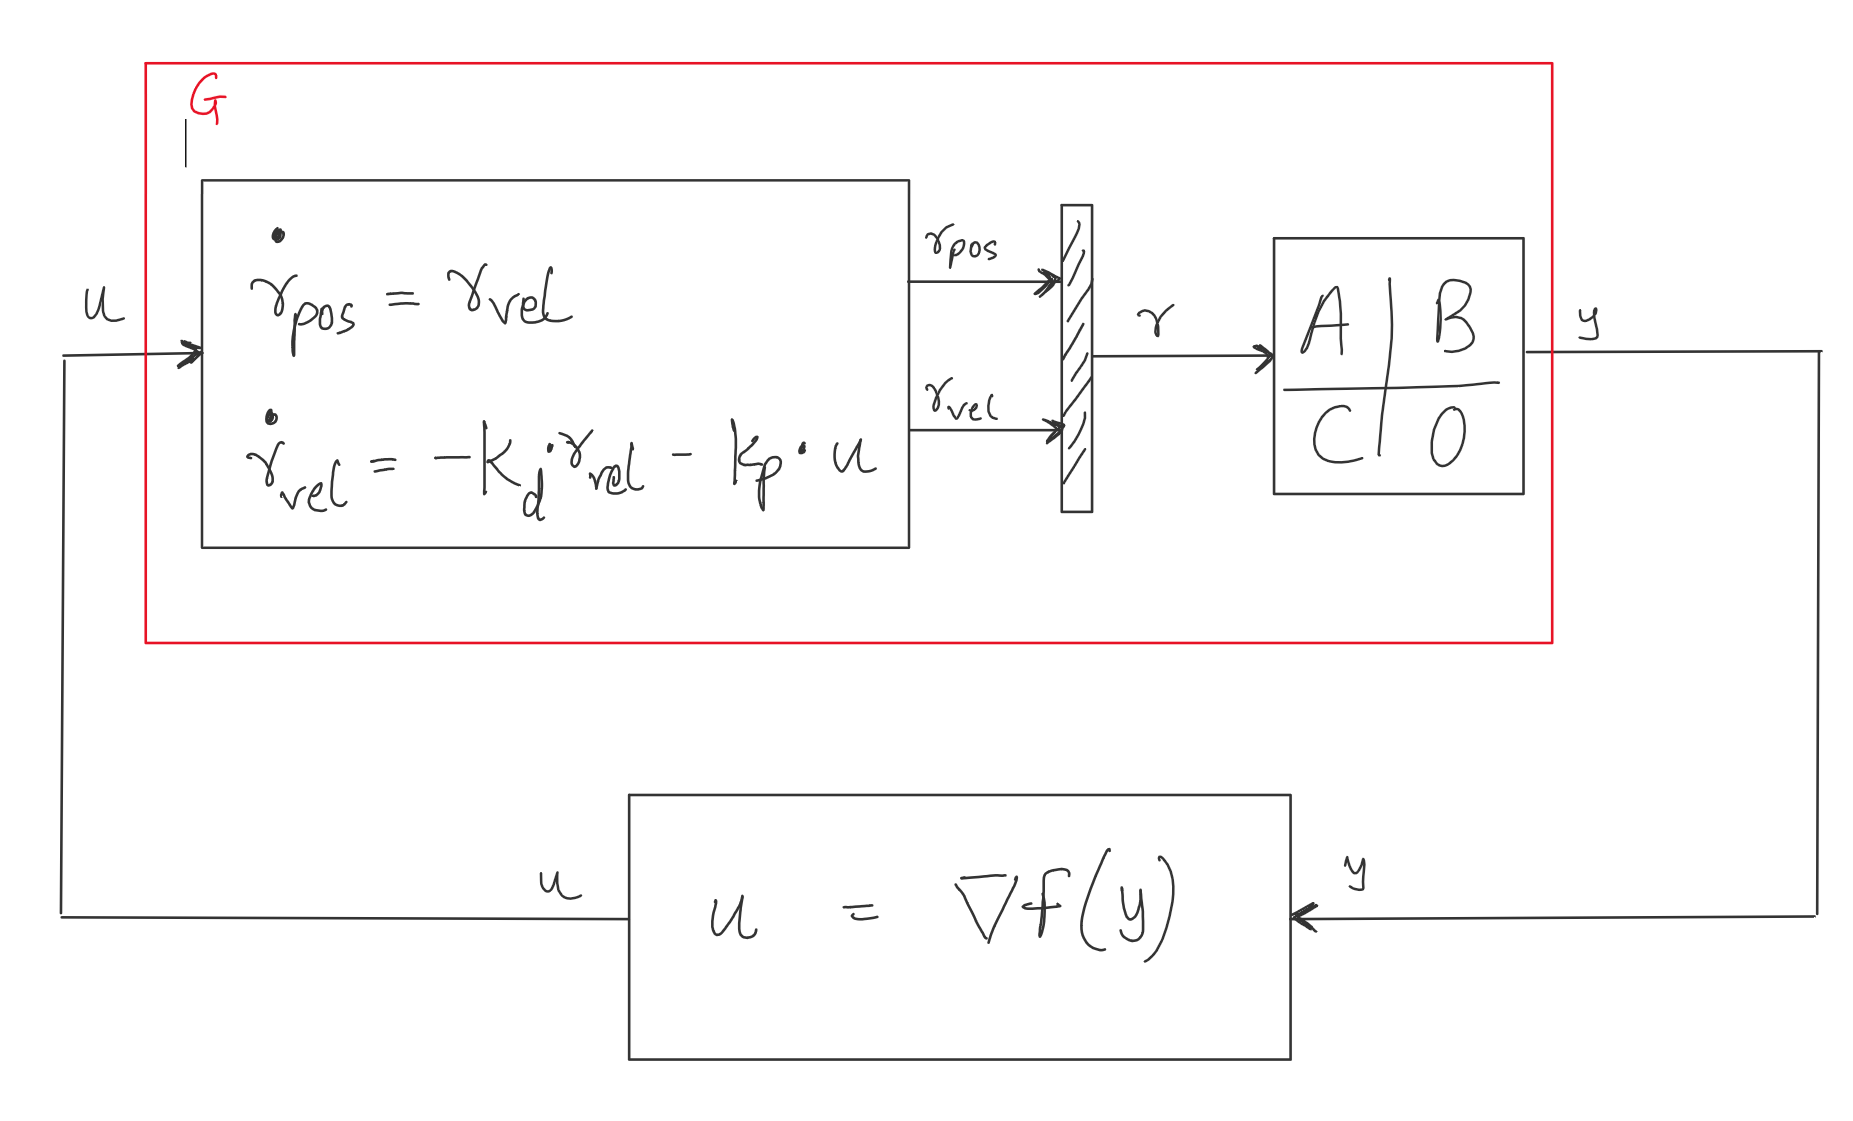
\includegraphics[width=8cm]{figures/Figure_IQC_paper.PNG}
		\centering
		% This file was created by matlab2tikz.
%
%The latest updates can be retrieved from
%  http://www.mathworks.com/matlabcentral/fileexchange/22022-matlab2tikz-matlab2tikz
%where you can also make suggestions and rate matlab2tikz.
%
\definecolor{mycolor1}{rgb}{0.09091,0.00000,0.90909}%
%
\begin{tikzpicture}

\begin{axis}[%
width=2.521in,
height=2.366in,
at={(0.758in,0.481in)},
scale only axis,
xmin=3,
xmax=30,
xlabel style={font=\color{white!15!black}},
xlabel={$k_d$},
ymin=0,
ymax=0.2,
ylabel style={font=\color{white!15!black}},
ylabel={$\alpha$},
axis background/.style={fill=white},
title style={font=\bfseries},
title={},
legend style={legend cell align=left, align=left, draw=white!15!black}
]
\addplot [color=red!0!mycolor1, dashed, line width=1.0pt]
  table[row sep=crcr]{%
1	-1\\
1.5	-1\\
2	-1\\
2.5	-1\\
3	-1\\
3.5	-1\\
4	-1\\
4.5	-1\\
5	-1\\
5.5	-1\\
6	0.001220703125\\
6.5	0.0311279296875\\
7	0.0579833984375\\
7.5	0.081787109375\\
8	0.103759765625\\
8.5	0.123291015625\\
9	0.140380859375\\
9.5	0.130615234375\\
10	0.1226806640625\\
10.5	0.1153564453125\\
11	0.108642578125\\
11.5	0.1025390625\\
12	0.09765625\\
12.5	0.0927734375\\
13	0.0885009765625\\
13.5	0.0848388671875\\
14	0.0811767578125\\
16	0.069580078125\\
18	0.06103515625\\
20	0.0543212890625\\
22	0.048828125\\
24	0.0445556640625\\
26	0.0408935546875\\
28	0.037841796875\\
};
\addlegendentry{$\delta=0$}
\addplot [color=black, line width=1.0pt, only marks, mark=o, mark options={solid, black}]
  table[row sep=crcr]{%
5	-0.07095539474729\\
7	0.0581605673803028\\
9	0.140995625810792\\
11	0.10888760621175\\
13	0.0889845777293038\\
15	0.0753353299872735\\
17	0.0653601305878092\\
19	0.0577389631460918\\
21	0.051720900936853\\
23	0.046845506606932\\
25	0.0428140844217267\\
27	0.0394241088254656\\
29	0.0365332709136337\\
};
\addlegendentry{Examples with $\delta=0$}


\addplot [color=red!50!mycolor1, line width=1.0pt]
  table[row sep=crcr]{%
1	-1\\
1.5	-1\\
2	-1\\
2.5	-1\\
3	-1\\
3.5	-1\\
4	-1\\
4.5	-1\\
5	-1\\
5.5	-1\\
6	-1\\
6.5	-1\\
7	-1\\
7.5	-1\\
8	-1\\
8.5	-1\\
9	-1\\
9.5	-1\\
10	-1\\
10.5	-1\\
11	-1\\
11.5	-1\\
12	0.003662109375\\
12.5	0.0152587890625\\
13	0.025634765625\\
13.5	0.035400390625\\
14	0.037841796875\\
14.5	0.0360107421875\\
15	0.0347900390625\\
15.5	0.0335693359375\\
16	0.0323486328125\\
16.5	0.03173828125\\
17	0.030517578125\\
17.5	0.0299072265625\\
18	0.0286865234375\\
18.5	0.028076171875\\
19	0.0274658203125\\
19.5	0.0262451171875\\
20	0.025634765625\\
20.5	0.0250244140625\\
21	0.0244140625\\
21.5	0.0238037109375\\
22	0.023193359375\\
22.5	0.0225830078125\\
23	0.02197265625\\
23.5	0.02197265625\\
24	0.0213623046875\\
24.5	0.020751953125\\
25	0.0201416015625\\
25.5	0.0201416015625\\
26	0.01953125\\
26.5	0.0189208984375\\
27	0.0189208984375\\
27.5	0.018310546875\\
28	0.018310546875\\
};
\addlegendentry{$\delta=0.5$}
\addplot [color=black, line width=1.25pt, draw=none, mark=asterisk, mark options={solid, black},only marks]
  table[row sep=crcr]{%
5	-0.199226365321045\\
7	-0.055972989506181\\
9	0.0401577268826836\\
11	0.0915509482192924\\
13	0.0732592079189861\\
15	0.0614669130668166\\
17	0.0548322584627636\\
19	0.0491797875201019\\
21	0.0442706506349314\\
23	0.0392183519500266\\
25	0.0363283142013289\\
27	0.0339632615215399\\
29	0.0308927840933636\\
};
\addlegendentry{Examples with $\delta=0.5$}
% \addplot [color=red!60!mycolor1, line width=1.0pt, forget plot]
%   table[row sep=crcr]{%
% 1	-1\\
% 1.5	-1\\
% 2	-1\\
% 2.5	-1\\
% 3	-1\\
% 3.5	-1\\
% 4	-1\\
% 4.5	-1\\
% 5	-1\\
% 5.5	-1\\
% 6	-1\\
% 6.5	-1\\
% 7	-1\\
% 7.5	-1\\
% 8	-1\\
% 8.5	-1\\
% 9	-1\\
% 9.5	-1\\
% 10	-1\\
% 10.5	-1\\
% 11	-1\\
% 11.5	-1\\
% 12	-1\\
% 12.5	-1\\
% 13	-1\\
% 13.5	-1\\
% 14	0.00732421875\\
% 14.5	0.0164794921875\\
% 15	0.0244140625\\
% 15.5	0.02685546875\\
% 16	0.025634765625\\
% 16.5	0.0250244140625\\
% 17	0.0244140625\\
% 17.5	0.023193359375\\
% 18	0.0225830078125\\
% 18.5	0.02197265625\\
% 19	0.0213623046875\\
% 19.5	0.020751953125\\
% 20	0.0201416015625\\
% 20.5	0.01953125\\
% 21	0.01953125\\
% 21.5	0.0189208984375\\
% 22	0.018310546875\\
% 22.5	0.0177001953125\\
% 23	0.0177001953125\\
% 23.5	0.01708984375\\
% 24	0.01708984375\\
% 24.5	0.0164794921875\\
% 25	0.015869140625\\
% 25.5	0.015869140625\\
% 26	0.0152587890625\\
% 26.5	0.0152587890625\\
% 27	0.0146484375\\
% 27.5	0.0146484375\\
% 28	0.0140380859375\\
% };
% \addplot [color=red!70!mycolor1, line width=1.0pt]
%   table[row sep=crcr]{%
% 1	-1\\
% 1.5	-1\\
% 2	-1\\
% 2.5	-1\\
% 3	-1\\
% 3.5	-1\\
% 4	-1\\
% 4.5	-1\\
% 5	-1\\
% 5.5	-1\\
% 6	-1\\
% 6.5	-1\\
% 7	-1\\
% 7.5	-1\\
% 8	-1\\
% 8.5	-1\\
% 9	-1\\
% 9.5	-1\\
% 10	-1\\
% 10.5	-1\\
% 11	-1\\
% 11.5	-1\\
% 12	-1\\
% 12.5	-1\\
% 13	-1\\
% 13.5	-1\\
% 14	-1\\
% 14.5	-1\\
% 15	-1\\
% 15.5	-1\\
% 16	0.0042724609375\\
% 16.5	0.010986328125\\
% 17	0.0177001953125\\
% 17.5	0.01708984375\\
% 18	0.01708984375\\
% 18.5	0.0164794921875\\
% 19	0.015869140625\\
% 19.5	0.0152587890625\\
% 20	0.0152587890625\\
% 20.5	0.0146484375\\
% 21	0.0140380859375\\
% 21.5	0.0140380859375\\
% 22	0.013427734375\\
% 22.5	0.013427734375\\
% 23	0.0128173828125\\
% 23.5	0.0128173828125\\
% 24	0.01220703125\\
% 24.5	0.01220703125\\
% 25	0.01220703125\\
% 25.5	0.0115966796875\\
% 26	0.0115966796875\\
% 26.5	0.010986328125\\
% 27	0.010986328125\\
% 27.5	0.010986328125\\
% 28	0.0103759765625\\
% };
% \addlegendentry{$\delta=0.7$}
% \addplot [color=red!80!mycolor1, line width=1.0pt, forget plot]
%   table[row sep=crcr]{%
% 1	-1\\
% 1.5	-1\\
% 2	-1\\
% 2.5	-1\\
% 3	-1\\
% 3.5	-1\\
% 4	-1\\
% 4.5	-1\\
% 5	-1\\
% 5.5	-1\\
% 6	-1\\
% 6.5	-1\\
% 7	-1\\
% 7.5	-1\\
% 8	-1\\
% 8.5	-1\\
% 9	-1\\
% 9.5	-1\\
% 10	-1\\
% 10.5	-1\\
% 11	-1\\
% 11.5	-1\\
% 12	-1\\
% 12.5	-1\\
% 13	-1\\
% 13.5	-1\\
% 14	-1\\
% 14.5	-1\\
% 15	-1\\
% 15.5	-1\\
% 16	-1\\
% 16.5	-1\\
% 17	-1\\
% 17.5	-1\\
% 18	-1\\
% 18.5	0.001220703125\\
% 19	0.0067138671875\\
% 19.5	0.0103759765625\\
% 20	0.009765625\\
% 20.5	0.009765625\\
% 21	0.0091552734375\\
% 21.5	0.0091552734375\\
% 22	0.0091552734375\\
% 22.5	0.008544921875\\
% 23	0.008544921875\\
% 23.5	0.008544921875\\
% 24	0.0079345703125\\
% 24.5	0.0079345703125\\
% 25	0.0079345703125\\
% 25.5	0.00732421875\\
% 26	0.00732421875\\
% 26.5	0.00732421875\\
% 27	0.00732421875\\
% 27.5	0.00732421875\\
% 28	0.0067138671875\\
% };
% \addplot [color=red!90!mycolor1, line width=1.0pt]
%   table[row sep=crcr]{%
% 1	-1\\
% 1.5	-1\\
% 2	-1\\
% 2.5	-1\\
% 3	-1\\
% 3.5	-1\\
% 4	-1\\
% 4.5	-1\\
% 5	-1\\
% 5.5	-1\\
% 6	-1\\
% 6.5	-1\\
% 7	-1\\
% 7.5	-1\\
% 8	-1\\
% 8.5	-1\\
% 9	-1\\
% 9.5	-1\\
% 10	-1\\
% 10.5	-1\\
% 11	-1\\
% 11.5	-1\\
% 12	-1\\
% 12.5	-1\\
% 13	-1\\
% 13.5	-1\\
% 14	-1\\
% 14.5	-1\\
% 15	-1\\
% 15.5	-1\\
% 16	-1\\
% 16.5	-1\\
% 17	-1\\
% 17.5	-1\\
% 18	-1\\
% 18.5	-1\\
% 19	-1\\
% 19.5	-1\\
% 20	-1\\
% 20.5	-1\\
% 21	-1\\
% 21.5	-1\\
% 22	-1\\
% 22.5	0.00244140625\\
% 23	0.0042724609375\\
% 23.5	0.003662109375\\
% 24	0.003662109375\\
% 24.5	0.003662109375\\
% 25	0.003662109375\\
% 25.5	0.003662109375\\
% 26	0.003662109375\\
% 26.5	0.0030517578125\\
% 27	0.0030517578125\\
% 27.5	0.0030517578125\\
% 28	0.0030517578125\\
% };
% \addlegendentry{$\delta=0.9$}
% \node[label={93:{}},circle,fill,inner sep=1.5pt] at (axis cs:7,0.0581) {};
% \node[label={45:{}},circle,fill,inner sep=1.5pt] at (axis cs:9,0.140996) {};
% \node[label={45:{}},circle,fill,inner sep=1.5pt] at (axis cs:16,0.0699893) {};
% \node[label={45:{}},circle,fill,inner sep=1.5pt] at (axis cs:25,0.04281) {};

% \node[label={45:{}},square,fill,inner sep=1.5pt] at (axis cs:9,0.0172) {};
% \node[label={45:{}},square,fill,inner sep=1.5pt] at (axis cs:11,0.0828) {};
% \node[label={45:{}},square,fill,inner sep=1.5pt] at (axis cs:16,0.0536) {};
% \node[label={45:{}},square,fill,inner sep=1.5pt] at (axis cs:25,0.0329) {};


% \node[label={45:{$A_2$}},circle,fill,inner sep=1.5pt] at (axis cs:16,0.0699893) {};
% \node[label={45:{$A_3$}},circle,fill,inner sep=1.5pt] at (axis cs:25,0.04281) {};
%\addplot [color=red, line width=1.0pt, forget plot]
%  table[row sep=crcr]{%
%1	-1\\
%1.5	-1\\
%2	-1\\
%2.5	-1\\
%3	-1\\
%3.5	-1\\
%4	-1\\
%4.5	-1\\
%5	-1\\
%5.5	-1\\
%6	-1\\
%6.5	-1\\
%7	-1\\
%7.5	-1\\
%8	-1\\
%8.5	-1\\
%9	-1\\
%9.5	-1\\
%10	-1\\
%10.5	-1\\
%11	-1\\
%11.5	-1\\
%12	-1\\
%12.5	-1\\
%13	-1\\
%13.5	-1\\
%14	-1\\
%14.5	-1\\
%15	-1\\
%15.5	-1\\
%16	-1\\
%16.5	-1\\
%17	-1\\
%17.5	-1\\
%18	-1\\
%18.5	-1\\
%19	-1\\
%19.5	-1\\
%20	-1\\
%20.5	-1\\
%21	-1\\
%21.5	-1\\
%22	-1\\
%22.5	-1\\
%23	-1\\
%23.5	-1\\
%24	-1\\
%24.5	-1\\
%25	-1\\
%25.5	-1\\
%26	-1\\
%26.5	-1\\
%27	-1\\
%27.5	-1\\
%28	-1\\
%};
\end{axis}

% \begin{axis}[%
% width=5.833in,
% height=4.375in,
% at={(0in,0in)},
% scale only axis,
% xmin=0,
% xmax=1,
% ymin=0,
% ymax=1,
% axis line style={draw=none},
% ticks=none,
% axis x line*=bottom,
% axis y line*=left
% ]
% \end{axis}
\end{tikzpicture}%
%		\caption{Conservatism analysis for quadrotor dynamics provided by first order ZF multipliers for $\psi \in \mathcal{S}(1,10)$ and varying $k_d$ with different bound $\delta \in \{0.1,0.2\cdots,0.9\}$ on the multiplicative noise (see Assumption \ref{assum:noise}).}
		\label{fig:quadrotor_optimal_kd_ZF_noisy_conservatism}
	\end{figure}
\end{frame}
%%%%%%%%%%%%%%%%%%%%%%%%%%%%%%%%%%%%%%%%%%%%%%%%%%%%%%%%%%%%%%%%%%%%%
\begin{frame}{Non-linear Friction Model}
	\begin{block}{Dynamics}
	\begin{equation}\label{eq:NLFsat}
		m\ddot{x}+b\vert\dot{x}\vert\dot{x} = u_F, 
	\end{equation}
	\end{block}
\begin{block}{qLPV representation}
\begin{equation}\label{eq:NLFssLPV}
	\begin{split}
		\begin{bmatrix} \dot{x}_{\textnormal{pos}}\\ \dot{x}_{\textnormal{vel}} \end{bmatrix} 
		&= 
		\begin{bmatrix} 0 & 1 \\ 0 & -\tfrac{b}{m}\rho \end{bmatrix} 
		\begin{bmatrix} x_{\textnormal{pos}}\\ x_{\textnormal{vel}} \end{bmatrix} 
		+
		\begin{bmatrix} 0 \\ \tfrac{1}{m} \end{bmatrix} 
		u_F
		\\[1mm]
		y
		&=
		\begin{bmatrix} 1 & 0 \end{bmatrix}
		\begin{bmatrix} x_{\textnormal{pos}}\\ x_{\textnormal{vel}} \end{bmatrix}
		\\[3mm]
		\rho(t) 
		&=
		\vert x_{\textnormal{vel}}(t)\vert,
		% \quad\rho :t \rightarrow \left[0,\,v_{\scaleto{\text{MAX}}{2.5pt}}\right]
	\end{split}
\end{equation}
\begin{block}{Synthesize an LPV controller on $\mathcal{P}=[0,5]$}
\end{block}
\end{block}
\end{frame}
%%%%%%%%%%%%%%%%%%%%%%%%%%%%%%%%%%%%%%%%%%%%%%%%%%%%%%%%%%%%%%%%%%%%%
\begin{frame}{Designing $k_d$ for largest convergence rate estimate $\alpha$}
	\begin{figure}[h!]
		\centering
		% This file was created by matlab2tikz.
%
%The latest updates can be retrieved from
%  http://www.mathworks.com/matlabcentral/fileexchange/22022-matlab2tikz-matlab2tikz
%where you can also make suggestions and rate matlab2tikz.
%
\definecolor{mycolor1}{rgb}{0.00000,0.44700,0.74100}%
\definecolor{mycolor2}{rgb}{0.85000,0.32500,0.09800}%
\definecolor{mycolor3}{rgb}{0.92900,0.69400,0.12500}%
\definecolor{mycolor4}{rgb}{0.49400,0.18400,0.55600}%
\definecolor{mycolor5}{rgb}{0.46600,0.67400,0.18800}%
\definecolor{mycolor6}{rgb}{0.30100,0.74500,0.93300}%
\definecolor{mycolor7}{rgb}{0.63500,0.07800,0.18400}%
%
\begin{tikzpicture}

\begin{axis}[%
width=2.4in,
height=2.4in,
at={(0.654in,0.509in)},
scale only axis,
xmin=0,
xmax=100,
xlabel style={font=\color{white!15!black}},
xlabel={$k_d$},
ymin=0,
ymax=0.04,
ylabel style={font=\color{white!15!black}},
ylabel={$\alpha$},
axis background/.style={fill=white},
title style={font=\bfseries},
%title={L=70},
xmajorgrids,
ymajorgrids,
legend style={at={(0.648,0.706)}, anchor=south west, legend cell align=left, align=left, draw=white!15!black,nodes={scale=0.75, transform shape}}
]
\addplot [color=mycolor1, line width=1.0pt]
  table[row sep=crcr]{%
1	0\\
1.5	0\\
2	0\\
2.5	0\\
3	0\\
3.5	0\\
4	0\\
4.5	0\\
5	0\\
5.5	0\\
6	0\\
6.5	0\\
7	0\\
7.5	0\\
8	0\\
8.5	0\\
9	0\\
9.5	0\\
10	0\\
10.5	0\\
11	0\\
11.5	0\\
12	0\\
12.5	0\\
13	0\\
13.5	0\\
14	0\\
14.5	0\\
15	0\\
15.5	0\\
16	0\\
16.5	0\\
17	0\\
17.5	0\\
18	0.03896484375\\
18.5	0.0391015625\\
19	0.0391015625\\
19.5	0.0391015625\\
20	0.0391015625\\
20.5	0.0391015625\\
21	0.0391015625\\
21.5	0.0391015625\\
22	0.0391015625\\
22.5	0.03896484375\\
23	0.03896484375\\
23.5	0.03896484375\\
24	0.038896484375\\
24.5	0.0385546875\\
25	0.03841796875\\
25.5	0.0380078125\\
26	0.0377685546875\\
26.5	0.0372216796875\\
27	0.03665771484375\\
27.5	0.0358203125\\
28	0.0352734375\\
28.5	0.0347265625\\
29	0.0341796875\\
29.5	0.0336328125\\
30	0.0330859375\\
30.5	0.0325390625\\
31	0.0319921875\\
31.5	0.0314453125\\
32	0.0308984375\\
32.5	0.030693359375\\
33	0.03021484375\\
33.5	0.02966796875\\
34	0.0292578125\\
34.5	0.0287109375\\
35	0.028505859375\\
35.5	0.02802734375\\
36	0.0276171875\\
36.5	0.0273480224609375\\
37	0.02693359375\\
37.5	0.0265234375\\
38	0.026258544921875\\
38.5	0.02583984375\\
39	0.0254296875\\
39.5	0.025224609375\\
40	0.0248828125\\
40.5	0.02462646484375\\
41	0.0243359375\\
41.5	0.024071044921875\\
42	0.0237890625\\
42.5	0.0232421875\\
43	0.02310546875\\
43.5	0.0226953125\\
44	0.0226953125\\
44.5	0.02243896484375\\
45	0.0221484375\\
45.5	0.021943359375\\
46	0.0216015625\\
46.5	0.02146484375\\
47	0.0210546875\\
47.5	0.02091796875\\
48	0.0208154296875\\
48.5	0.0205078125\\
49	0.02037109375\\
49.5	0.0199609375\\
50	0.0199609375\\
50.5	0.019755859375\\
51	0.0194140625\\
51.5	0.01927734375\\
52	0.019208984375\\
52.5	0.0188671875\\
53	0.01873046875\\
53.5	0.0186279296875\\
54	0.0183203125\\
54.5	0.0183203125\\
55	0.018115234375\\
55.5	0.0177734375\\
56	0.0177734375\\
56.5	0.01763671875\\
57	0.01751708984375\\
57.5	0.0172265625\\
58	0.0172265625\\
58.5	0.017021484375\\
59	0.0166796875\\
59.5	0.0166796875\\
60	0.01654296875\\
60.5	0.016474609375\\
61	0.0161328125\\
61.5	0.0161328125\\
62	0.01599609375\\
62.5	0.015927734375\\
63	0.0158615112304688\\
63.5	0.0155859375\\
64	0.0155859375\\
64.5	0.01544921875\\
65	0.0153466796875\\
65.5	0.0150390625\\
66	0.0150390625\\
66.5	0.01490234375\\
67	0.01490234375\\
67.5	0.0147998046875\\
68	0.0144921875\\
68.5	0.0144921875\\
69	0.01435546875\\
69.5	0.01435546875\\
70	0.0142529296875\\
70.5	0.0139453125\\
71	0.0139453125\\
71.5	0.0139453125\\
72	0.01380859375\\
72.5	0.013740234375\\
73	0.01368896484375\\
73.5	0.0133984375\\
74	0.0133984375\\
74.5	0.0133984375\\
75	0.01326171875\\
75.5	0.013193359375\\
76	0.01314208984375\\
76.5	0.0128515625\\
77	0.0128515625\\
77.5	0.0128515625\\
78	0.01271484375\\
78.5	0.01271484375\\
79	0.012646484375\\
79.5	0.0123046875\\
80	0.0123046875\\
80.5	0.0123046875\\
81	0.0123046875\\
81.5	0.01216796875\\
82	0.01216796875\\
82.5	0.012099609375\\
83	0.0120355224609375\\
83.5	0.0117578125\\
84	0.0117578125\\
84.5	0.0117578125\\
85	0.01162109375\\
85.5	0.01162109375\\
86	0.01162109375\\
86.5	0.0115185546875\\
87	0.0112109375\\
87.5	0.0112109375\\
88	0.0112109375\\
88.5	0.0112109375\\
89	0.0112109375\\
89.5	0.01107421875\\
90	0.01107421875\\
90.5	0.011005859375\\
91	0.0109716796875\\
91.5	0.0106640625\\
92	0.0106640625\\
92.5	0.0106640625\\
93	0.0106640625\\
93.5	0.0106640625\\
94	0.01052734375\\
94.5	0.01052734375\\
95	0.010458984375\\
95.5	0.0104248046875\\
96	0.01040771484375\\
96.5	0.0101171875\\
97	0.0101171875\\
97.5	0.0101171875\\
98	0.0101171875\\
98.5	0.0101171875\\
99	0.00998046875\\
99.5	0.00998046875\\
100	0.00998046875\\
};
\addlegendentry{$\delta\text{ = 0}$}

% \addplot [color=mycolor2, line width=1.0pt]
%   table[row sep=crcr]{%
% 1	0\\
% 1.5	0\\
% 2	0\\
% 2.5	0\\
% 3	0\\
% 3.5	0\\
% 4	0\\
% 4.5	0\\
% 5	0\\
% 5.5	0\\
% 6	0\\
% 6.5	0\\
% 7	0\\
% 7.5	0\\
% 8	0\\
% 8.5	0\\
% 9	0\\
% 9.5	0\\
% 10	0\\
% 10.5	0\\
% 11	0\\
% 11.5	0\\
% 12	0\\
% 12.5	0\\
% 13	0\\
% 13.5	0\\
% 14	0\\
% 14.5	0\\
% 15	0\\
% 15.5	0\\
% 16	0\\
% 16.5	0\\
% 17	0\\
% 17.5	0\\
% 18	0\\
% 18.5	0\\
% 19	0\\
% 19.5	0\\
% 20	0.0360980224609375\\
% 20.5	0.03841796875\\
% 21	0.0385546875\\
% 21.5	0.03841796875\\
% 22	0.03841796875\\
% 22.5	0.0380078125\\
% 23	0.03787109375\\
% 23.5	0.03732421875\\
% 24	0.0369140625\\
% 24.5	0.0363671875\\
% 25	0.035615234375\\
% 25.5	0.035068359375\\
% 26	0.0344541931152344\\
% 26.5	0.0336328125\\
% 27	0.0330859375\\
% 27.5	0.0325390625\\
% 28	0.0319921875\\
% 28.5	0.0314453125\\
% 29	0.0308984375\\
% 29.5	0.0303515625\\
% 30	0.0298046875\\
% 30.5	0.0292578125\\
% 31	0.028992919921875\\
% 31.5	0.028505859375\\
% 32	0.02802734375\\
% 32.5	0.0276171875\\
% 33	0.0270703125\\
% 33.5	0.0268310546875\\
% 34	0.02638671875\\
% 34.5	0.0259765625\\
% 35	0.0254296875\\
% 35.5	0.02529296875\\
% 36	0.0248828125\\
% 36.5	0.02462646484375\\
% 37	0.02419921875\\
% 37.5	0.0237890625\\
% 38	0.02365234375\\
% 38.5	0.0232421875\\
% 39	0.023037109375\\
% 39.5	0.0226953125\\
% 40	0.0224560546875\\
% 40.5	0.0221484375\\
% 41	0.0219091796875\\
% 41.5	0.0216015625\\
% 42	0.021396484375\\
% 42.5	0.0210546875\\
% 43	0.02091796875\\
% 43.5	0.0205078125\\
% 44	0.02037109375\\
% 44.5	0.0199609375\\
% 45	0.0199609375\\
% 45.5	0.019755859375\\
% 46	0.0194140625\\
% 46.5	0.01927734375\\
% 47	0.0191416931152344\\
% 47.5	0.0188671875\\
% 48	0.01873046875\\
% 48.5	0.0183203125\\
% 49	0.0183203125\\
% 49.5	0.018115234375\\
% 50	0.0177734375\\
% 50.5	0.0177734375\\
% 51	0.01763671875\\
% 51.5	0.0172265625\\
% 52	0.0172265625\\
% 52.5	0.01708984375\\
% 53	0.016961669921875\\
% 53.5	0.0166796875\\
% 54	0.01654296875\\
% 54.5	0.016474609375\\
% 55	0.0161328125\\
% 55.5	0.0161328125\\
% 56	0.01599609375\\
% 56.5	0.0158935546875\\
% 57	0.0155859375\\
% 57.5	0.0155859375\\
% 58	0.01544921875\\
% 58.5	0.015380859375\\
% 59	0.0150390625\\
% 59.5	0.0150390625\\
% 60	0.01490234375\\
% 60.5	0.014833984375\\
% 61	0.0144921875\\
% 61.5	0.0144921875\\
% 62	0.0144921875\\
% 62.5	0.01435546875\\
% 63	0.0142529296875\\
% 63.5	0.0139453125\\
% 64	0.0139453125\\
% 64.5	0.0139453125\\
% 65	0.01380859375\\
% 65.5	0.0137060546875\\
% 66	0.0133984375\\
% 66.5	0.0133984375\\
% 67	0.0133984375\\
% 67.5	0.01326171875\\
% 68	0.013193359375\\
% 68.5	0.013133544921875\\
% 69	0.0128515625\\
% 69.5	0.0128515625\\
% 70	0.0128515625\\
% 70.5	0.01271484375\\
% 71	0.012646484375\\
% 71.5	0.0125823974609375\\
% 72	0.0123046875\\
% 72.5	0.0123046875\\
% 73	0.0123046875\\
% 73.5	0.01216796875\\
% 74	0.012099609375\\
% 74.5	0.0120654296875\\
% 75	0.0117578125\\
% 75.5	0.0117578125\\
% 76	0.0117578125\\
% 76.5	0.0117578125\\
% 77	0.01162109375\\
% 77.5	0.011552734375\\
% 78	0.0115185546875\\
% 78.5	0.0112109375\\
% 79	0.0112109375\\
% 79.5	0.0112109375\\
% 80	0.0112109375\\
% 80.5	0.01107421875\\
% 81	0.01107421875\\
% 81.5	0.011005859375\\
% 82	0.0109716796875\\
% 82.5	0.0106640625\\
% 83	0.0106640625\\
% 83.5	0.0106640625\\
% 84	0.0106640625\\
% 84.5	0.01052734375\\
% 85	0.01052734375\\
% 85.5	0.010458984375\\
% 86	0.010458984375\\
% 86.5	0.010399169921875\\
% 87	0.0101171875\\
% 87.5	0.0101171875\\
% 88	0.0101171875\\
% 88.5	0.0101171875\\
% 89	0.00998046875\\
% 89.5	0.00998046875\\
% 90	0.00998046875\\
% 90.5	0.009912109375\\
% 91	0.0098779296875\\
% 91.5	0.0095703125\\
% 92	0.0095703125\\
% 92.5	0.0095703125\\
% 93	0.0095703125\\
% 93.5	0.0095703125\\
% 94	0.0095703125\\
% 94.5	0.00943359375\\
% 95	0.00943359375\\
% 95.5	0.009365234375\\
% 96	0.009365234375\\
% 96.5	0.00931396484375\\
% 97	0.0090234375\\
% 97.5	0.0090234375\\
% 98	0.0090234375\\
% 98.5	0.0090234375\\
% 99	0.0090234375\\
% 99.5	0.0090234375\\
% 100	0.00888671875\\
% };
% \addlegendentry{$\delta\text{ = 0.1}$}

% \addplot [color=mycolor3, line width=1.0pt]
%   table[row sep=crcr]{%
% 1	0\\
% 1.5	0\\
% 2	0\\
% 2.5	0\\
% 3	0\\
% 3.5	0\\
% 4	0\\
% 4.5	0\\
% 5	0\\
% 5.5	0\\
% 6	0\\
% 6.5	0\\
% 7	0\\
% 7.5	0\\
% 8	0\\
% 8.5	0\\
% 9	0\\
% 9.5	0\\
% 10	0\\
% 10.5	0\\
% 11	0\\
% 11.5	0\\
% 12	0\\
% 12.5	0\\
% 13	0\\
% 13.5	0\\
% 14	0\\
% 14.5	0\\
% 15	0\\
% 15.5	0\\
% 16	0\\
% 16.5	0\\
% 17	0\\
% 17.5	0\\
% 18	0\\
% 18.5	0\\
% 19	0\\
% 19.5	0\\
% 20	0\\
% 20.5	0\\
% 21	0\\
% 21.5	0\\
% 22	0.0265234375\\
% 22.5	0.03513671875\\
% 23	0.034521484375\\
% 23.5	0.0336328125\\
% 24	0.0330859375\\
% 24.5	0.0325390625\\
% 25	0.03185546875\\
% 25.5	0.031240234375\\
% 26	0.0306591796875\\
% 26.5	0.0301123046875\\
% 27	0.0295654296875\\
% 27.5	0.0290185546875\\
% 28	0.028505859375\\
% 28.5	0.02802734375\\
% 29	0.02748046875\\
% 29.5	0.0270703125\\
% 30	0.0265234375\\
% 30.5	0.0259765625\\
% 31	0.025771484375\\
% 31.5	0.02529296875\\
% 32	0.0248828125\\
% 32.5	0.0243359375\\
% 33	0.02419921875\\
% 33.5	0.0237890625\\
% 34	0.0235166931152344\\
% 34.5	0.02310546875\\
% 35	0.0226953125\\
% 35.5	0.022490234375\\
% 36	0.0221484375\\
% 36.5	0.02189208984375\\
% 37	0.0216015625\\
% 37.5	0.0210546875\\
% 38	0.02091796875\\
% 38.5	0.0205078125\\
% 39	0.02037109375\\
% 39.5	0.020242919921875\\
% 40	0.0199609375\\
% 40.5	0.0197216796875\\
% 41	0.0194140625\\
% 41.5	0.019208984375\\
% 42	0.0188671875\\
% 42.5	0.01873046875\\
% 43	0.0185958862304688\\
% 43.5	0.0183203125\\
% 44	0.018115234375\\
% 44.5	0.0177734375\\
% 45	0.0177734375\\
% 45.5	0.017568359375\\
% 46	0.0172265625\\
% 46.5	0.01708984375\\
% 47	0.01697021484375\\
% 47.5	0.0166796875\\
% 48	0.01654296875\\
% 48.5	0.016474609375\\
% 49	0.0161328125\\
% 49.5	0.0161328125\\
% 50	0.01599609375\\
% 50.5	0.0155859375\\
% 51	0.0155859375\\
% 51.5	0.01544921875\\
% 52	0.015380859375\\
% 52.5	0.0150390625\\
% 53	0.0150390625\\
% 53.5	0.01490234375\\
% 54	0.0147998046875\\
% 54.5	0.0144921875\\
% 55	0.0144921875\\
% 55.5	0.01435546875\\
% 56	0.0142529296875\\
% 56.5	0.0139453125\\
% 57	0.0139453125\\
% 57.5	0.01380859375\\
% 58	0.013740234375\\
% 58.5	0.0133984375\\
% 59	0.0133984375\\
% 59.5	0.0133984375\\
% 60	0.01326171875\\
% 60.5	0.013193359375\\
% 61	0.0128515625\\
% 61.5	0.0128515625\\
% 62	0.0128515625\\
% 62.5	0.01271484375\\
% 63	0.012646484375\\
% 63.5	0.012586669921875\\
% 64	0.0123046875\\
% 64.5	0.0123046875\\
% 65	0.01216796875\\
% 65.5	0.01216796875\\
% 66	0.012099609375\\
% 66.5	0.0117578125\\
% 67	0.0117578125\\
% 67.5	0.0117578125\\
% 68	0.0117578125\\
% 68.5	0.01162109375\\
% 69	0.011552734375\\
% 69.5	0.01150146484375\\
% 70	0.0112109375\\
% 70.5	0.0112109375\\
% 71	0.0112109375\\
% 71.5	0.01107421875\\
% 72	0.01107421875\\
% 72.5	0.011005859375\\
% 73	0.01095458984375\\
% 73.5	0.0106640625\\
% 74	0.0106640625\\
% 74.5	0.0106640625\\
% 75	0.0106640625\\
% 75.5	0.01052734375\\
% 76	0.010458984375\\
% 76.5	0.0104248046875\\
% 77	0.0101171875\\
% 77.5	0.0101171875\\
% 78	0.0101171875\\
% 78.5	0.0101171875\\
% 79	0.0101171875\\
% 79.5	0.00998046875\\
% 80	0.009912109375\\
% 80.5	0.009912109375\\
% 81	0.009852294921875\\
% 81.5	0.0095703125\\
% 82	0.0095703125\\
% 82.5	0.0095703125\\
% 83	0.0095703125\\
% 83.5	0.0095703125\\
% 84	0.00943359375\\
% 84.5	0.00943359375\\
% 85	0.009365234375\\
% 85.5	0.0093310546875\\
% 86	0.0093011474609375\\
% 86.5	0.0090234375\\
% 87	0.0090234375\\
% 87.5	0.0090234375\\
% 88	0.0090234375\\
% 88.5	0.0090234375\\
% 89	0.00888671875\\
% 89.5	0.00888671875\\
% 90	0.00888671875\\
% 90.5	0.008818359375\\
% 91	0.0084765625\\
% 91.5	0.0084765625\\
% 92	0.0084765625\\
% 92.5	0.0084765625\\
% 93	0.0084765625\\
% 93.5	0.0084765625\\
% 94	0.0084765625\\
% 94.5	0.00833984375\\
% 95	0.00833984375\\
% 95.5	0.00833984375\\
% 96	0.008271484375\\
% 96.5	0.008271484375\\
% 97	0.0082373046875\\
% 97.5	0.00820419311523438\\
% 98	0.0079296875\\
% 98.5	0.0079296875\\
% 99	0.0079296875\\
% 99.5	0.0079296875\\
% 100	0.0079296875\\
% };
% \addlegendentry{$\delta\text{ = 0.2}$}

\addplot [color=mycolor5, line width=1.0pt]
  table[row sep=crcr]{%
1	0\\
1.5	0\\
2	0\\
2.5	0\\
3	0\\
3.5	0\\
4	0\\
4.5	0\\
5	0\\
5.5	0\\
6	0\\
6.5	0\\
7	0\\
7.5	0\\
8	0\\
8.5	0\\
9	0\\
9.5	0\\
10	0\\
10.5	0\\
11	0\\
11.5	0\\
12	0\\
12.5	0\\
13	0\\
13.5	0\\
14	0\\
14.5	0\\
15	0\\
15.5	0\\
16	0\\
16.5	0\\
17	0\\
17.5	0\\
18	0\\
18.5	0\\
19	0\\
19.5	0\\
20	0\\
20.5	0\\
21	0\\
21.5	0\\
22	0\\
22.5	0\\
23	0\\
23.5	0\\
24	0.01162109375\\
24.5	0.0284716796875\\
25	0.027958984375\\
25.5	0.0273779296875\\
26	0.026865234375\\
26.5	0.02638671875\\
27	0.02583984375\\
27.5	0.0254296875\\
28	0.0248828125\\
28.5	0.0243359375\\
29	0.0240966796875\\
29.5	0.02365234375\\
30	0.0232421875\\
30.5	0.0226953125\\
31	0.022490234375\\
31.5	0.0221484375\\
32	0.0216015625\\
32.5	0.02146484375\\
33	0.0210546875\\
33.5	0.020849609375\\
34	0.0205078125\\
34.5	0.0202685546875\\
35	0.0199609375\\
35.5	0.01970458984375\\
36	0.0194140625\\
36.5	0.01915771484375\\
37	0.0188671875\\
37.5	0.0186279296875\\
38	0.0183203125\\
38.5	0.018115234375\\
39	0.0177734375\\
39.5	0.01763671875\\
40	0.0172265625\\
40.5	0.0172265625\\
41	0.017021484375\\
41.5	0.0166796875\\
42	0.01654296875\\
42.5	0.0164404296875\\
43	0.0161328125\\
43.5	0.01599609375\\
44	0.01587646484375\\
44.5	0.0155859375\\
45	0.01544921875\\
45.5	0.0153466796875\\
46	0.0150390625\\
46.5	0.0150390625\\
47	0.014833984375\\
47.5	0.0144921875\\
48	0.0144921875\\
48.5	0.01435546875\\
49	0.0142529296875\\
49.5	0.0139453125\\
50	0.0139453125\\
50.5	0.01380859375\\
51	0.0137060546875\\
51.5	0.0133984375\\
52	0.0133984375\\
52.5	0.01326171875\\
53	0.0131591796875\\
53.5	0.0128515625\\
54	0.0128515625\\
54.5	0.01271484375\\
55	0.01271484375\\
55.5	0.01259521484375\\
56	0.0123046875\\
56.5	0.0123046875\\
57	0.01216796875\\
57.5	0.012099609375\\
58	0.0120654296875\\
58.5	0.0117578125\\
59	0.0117578125\\
59.5	0.0117578125\\
60	0.01162109375\\
60.5	0.011552734375\\
61	0.0112109375\\
61.5	0.0112109375\\
62	0.0112109375\\
62.5	0.01107421875\\
63	0.01107421875\\
63.5	0.011005859375\\
64	0.0106640625\\
64.5	0.0106640625\\
65	0.0106640625\\
65.5	0.0106640625\\
66	0.01052734375\\
66.5	0.010458984375\\
67	0.0104248046875\\
67.5	0.0101171875\\
68	0.0101171875\\
68.5	0.0101171875\\
69	0.0101171875\\
69.5	0.00998046875\\
70	0.00998046875\\
70.5	0.009912109375\\
71	0.009852294921875\\
71.5	0.0095703125\\
72	0.0095703125\\
72.5	0.0095703125\\
73	0.0095703125\\
73.5	0.00943359375\\
74	0.00943359375\\
74.5	0.009365234375\\
75	0.0093310546875\\
75.5	0.0090234375\\
76	0.0090234375\\
76.5	0.0090234375\\
77	0.0090234375\\
77.5	0.0090234375\\
78	0.00888671875\\
78.5	0.00888671875\\
79	0.008818359375\\
79.5	0.0087841796875\\
80	0.0084765625\\
80.5	0.0084765625\\
81	0.0084765625\\
81.5	0.0084765625\\
82	0.0084765625\\
82.5	0.0084765625\\
83	0.00833984375\\
83.5	0.00833984375\\
84	0.008271484375\\
84.5	0.008271484375\\
85	0.00822021484375\\
85.5	0.0079296875\\
86	0.0079296875\\
86.5	0.0079296875\\
87	0.0079296875\\
87.5	0.0079296875\\
88	0.0079296875\\
88.5	0.00779296875\\
89	0.00779296875\\
89.5	0.00779296875\\
90	0.007724609375\\
90.5	0.007724609375\\
91	0.00767333984375\\
91.5	0.0073828125\\
92	0.0073828125\\
92.5	0.0073828125\\
93	0.0073828125\\
93.5	0.0073828125\\
94	0.0073828125\\
94.5	0.0073828125\\
95	0.00724609375\\
95.5	0.00724609375\\
96	0.00724609375\\
96.5	0.00724609375\\
97	0.007177734375\\
97.5	0.0071435546875\\
98	0.00712646484375\\
98.5	0.0068359375\\
99	0.0068359375\\
99.5	0.0068359375\\
100	0.0068359375\\
};
\addlegendentry{$\delta\text{ = 0.3}$}

% \addplot [color=mycolor5, line width=1.0pt]
%   table[row sep=crcr]{%
% 1	0\\
% 1.5	0\\
% 2	0\\
% 2.5	0\\
% 3	0\\
% 3.5	0\\
% 4	0\\
% 4.5	0\\
% 5	0\\
% 5.5	0\\
% 6	0\\
% 6.5	0\\
% 7	0\\
% 7.5	0\\
% 8	0\\
% 8.5	0\\
% 9	0\\
% 9.5	0\\
% 10	0\\
% 10.5	0\\
% 11	0\\
% 11.5	0\\
% 12	0\\
% 12.5	0\\
% 13	0\\
% 13.5	0\\
% 14	0\\
% 14.5	0\\
% 15	0\\
% 15.5	0\\
% 16	0\\
% 16.5	0\\
% 17	0\\
% 17.5	0\\
% 18	0\\
% 18.5	0\\
% 19	0\\
% 19.5	0\\
% 20	0\\
% 20.5	0\\
% 21	0\\
% 21.5	0\\
% 22	0\\
% 22.5	0\\
% 23	0\\
% 23.5	0\\
% 24	0\\
% 24.5	0\\
% 25	0\\
% 25.5	0\\
% 26	0\\
% 26.5	0.0221484375\\
% 27	0.0221484375\\
% 27.5	0.0216015625\\
% 28	0.021396484375\\
% 28.5	0.02091796875\\
% 29	0.0205078125\\
% 29.5	0.0202685546875\\
% 30	0.0199609375\\
% 30.5	0.0194140625\\
% 31	0.01927734375\\
% 31.5	0.0188671875\\
% 32	0.018662109375\\
% 32.5	0.0183203125\\
% 33	0.018115234375\\
% 33.5	0.0177734375\\
% 34	0.01763671875\\
% 34.5	0.0172265625\\
% 35	0.01708984375\\
% 35.5	0.0166796875\\
% 36	0.01654296875\\
% 36.5	0.0161328125\\
% 37	0.01599609375\\
% 37.5	0.01599609375\\
% 38	0.0155859375\\
% 38.5	0.01544921875\\
% 39	0.015380859375\\
% 39.5	0.0150390625\\
% 40	0.01490234375\\
% 40.5	0.0147998046875\\
% 41	0.0144921875\\
% 41.5	0.01435546875\\
% 42	0.0142529296875\\
% 42.5	0.0139453125\\
% 43	0.0139453125\\
% 43.5	0.013740234375\\
% 44	0.0133984375\\
% 44.5	0.0133984375\\
% 45	0.01326171875\\
% 45.5	0.0131591796875\\
% 46	0.0128515625\\
% 46.5	0.0128515625\\
% 47	0.01271484375\\
% 47.5	0.0126123046875\\
% 48	0.0123046875\\
% 48.5	0.0123046875\\
% 49	0.01216796875\\
% 49.5	0.012099609375\\
% 50	0.0117578125\\
% 50.5	0.0117578125\\
% 51	0.0117578125\\
% 51.5	0.01162109375\\
% 52	0.0115185546875\\
% 52.5	0.0112109375\\
% 53	0.0112109375\\
% 53.5	0.0112109375\\
% 54	0.01107421875\\
% 54.5	0.011005859375\\
% 55	0.0106640625\\
% 55.5	0.0106640625\\
% 56	0.0106640625\\
% 56.5	0.01052734375\\
% 57	0.010458984375\\
% 57.5	0.0104248046875\\
% 58	0.0101171875\\
% 58.5	0.0101171875\\
% 59	0.0101171875\\
% 59.5	0.00998046875\\
% 60	0.00998046875\\
% 60.5	0.009912109375\\
% 61	0.0095703125\\
% 61.5	0.0095703125\\
% 62	0.0095703125\\
% 62.5	0.0095703125\\
% 63	0.00943359375\\
% 63.5	0.00943359375\\
% 64	0.0093310546875\\
% 64.5	0.0093011474609375\\
% 65	0.0090234375\\
% 65.5	0.0090234375\\
% 66	0.0090234375\\
% 66.5	0.00888671875\\
% 67	0.00888671875\\
% 67.5	0.00888671875\\
% 68	0.008818359375\\
% 68.5	0.008758544921875\\
% 69	0.0084765625\\
% 69.5	0.0084765625\\
% 70	0.0084765625\\
% 70.5	0.0084765625\\
% 71	0.00833984375\\
% 71.5	0.00833984375\\
% 72	0.008271484375\\
% 72.5	0.008271484375\\
% 73	0.008211669921875\\
% 73.5	0.0079296875\\
% 74	0.0079296875\\
% 74.5	0.0079296875\\
% 75	0.0079296875\\
% 75.5	0.0079296875\\
% 76	0.00779296875\\
% 76.5	0.00779296875\\
% 77	0.007724609375\\
% 77.5	0.007724609375\\
% 78	0.0073828125\\
% 78.5	0.0073828125\\
% 79	0.0073828125\\
% 79.5	0.0073828125\\
% 80	0.0073828125\\
% 80.5	0.0073828125\\
% 81	0.0073828125\\
% 81.5	0.00724609375\\
% 82	0.00724609375\\
% 82.5	0.00724609375\\
% 83	0.007177734375\\
% 83.5	0.007177734375\\
% 84	0.00712646484375\\
% 84.5	0.0068359375\\
% 85	0.0068359375\\
% 85.5	0.0068359375\\
% 86	0.0068359375\\
% 86.5	0.0068359375\\
% 87	0.0068359375\\
% 87.5	0.0068359375\\
% 88	0.00669921875\\
% 88.5	0.00669921875\\
% 89	0.00669921875\\
% 89.5	0.00669921875\\
% 90	0.006630859375\\
% 90.5	0.0065966796875\\
% 91	0.00657958984375\\
% 91.5	0.0062890625\\
% 92	0.0062890625\\
% 92.5	0.0062890625\\
% 93	0.0062890625\\
% 93.5	0.0062890625\\
% 94	0.0062890625\\
% 94.5	0.0062890625\\
% 95	0.0062890625\\
% 95.5	0.00615234375\\
% 96	0.00615234375\\
% 96.5	0.00615234375\\
% 97	0.00615234375\\
% 97.5	0.00615234375\\
% 98	0.006083984375\\
% 98.5	0.006083984375\\
% 99	0.0060498046875\\
% 99.5	0.006024169921875\\
% 100	0.0057421875\\
% };
% \addlegendentry{$\delta\text{ = 0.4}$}

\addplot [color=mycolor7, line width=1.0pt]
  table[row sep=crcr]{%
1	0\\
1.5	0\\
2	0\\
2.5	0\\
3	0\\
3.5	0\\
4	0\\
4.5	0\\
5	0\\
5.5	0\\
6	0\\
6.5	0\\
7	0\\
7.5	0\\
8	0\\
8.5	0\\
9	0\\
9.5	0\\
10	0\\
10.5	0\\
11	0\\
11.5	0\\
12	0\\
12.5	0\\
13	0\\
13.5	0\\
14	0\\
14.5	0\\
15	0\\
15.5	0\\
16	0\\
16.5	0\\
17	0\\
17.5	0\\
18	0\\
18.5	0\\
19	0\\
19.5	0\\
20	0\\
20.5	0\\
21	0\\
21.5	0\\
22	0\\
22.5	0\\
23	0\\
23.5	0\\
24	0\\
24.5	0\\
25	0\\
25.5	0\\
26	0\\
26.5	0\\
27	0\\
27.5	0\\
28	0\\
28.5	0\\
29	0.01708984375\\
29.5	0.0166796875\\
30	0.01654296875\\
30.5	0.0161328125\\
31	0.01599609375\\
31.5	0.015867919921875\\
32	0.0155859375\\
32.5	0.015380859375\\
33	0.01490234375\\
33.5	0.01490234375\\
34	0.0144921875\\
34.5	0.01435546875\\
35	0.0142529296875\\
35.5	0.0139453125\\
36	0.01380859375\\
36.5	0.01368896484375\\
37	0.0133984375\\
37.5	0.01326171875\\
38	0.01314208984375\\
38.5	0.0128515625\\
39	0.01271484375\\
39.5	0.012646484375\\
40	0.0123046875\\
40.5	0.0123046875\\
41	0.01216796875\\
41.5	0.012039794921875\\
42	0.0117578125\\
42.5	0.0117578125\\
43	0.01162109375\\
43.5	0.011492919921875\\
44	0.0112109375\\
44.5	0.0112109375\\
45	0.01107421875\\
45.5	0.0109716796875\\
46	0.0106640625\\
46.5	0.0106640625\\
47	0.01052734375\\
47.5	0.010458984375\\
48	0.01040771484375\\
48.5	0.0101171875\\
49	0.0101171875\\
49.5	0.00998046875\\
50	0.00998046875\\
50.5	0.0098779296875\\
51	0.0095703125\\
51.5	0.0095703125\\
52	0.0095703125\\
52.5	0.00943359375\\
53	0.009365234375\\
53.5	0.0093310546875\\
54	0.0090234375\\
54.5	0.0090234375\\
55	0.0090234375\\
55.5	0.00888671875\\
56	0.00888671875\\
56.5	0.008818359375\\
57	0.00876708984375\\
57.5	0.0084765625\\
58	0.0084765625\\
58.5	0.0084765625\\
59	0.00833984375\\
59.5	0.00833984375\\
60	0.008271484375\\
60.5	0.0082373046875\\
61	0.0079296875\\
61.5	0.0079296875\\
62	0.0079296875\\
62.5	0.0079296875\\
63	0.00779296875\\
63.5	0.00779296875\\
64	0.00779296875\\
64.5	0.007724609375\\
65	0.00767333984375\\
65.5	0.0073828125\\
66	0.0073828125\\
66.5	0.0073828125\\
67	0.0073828125\\
67.5	0.0073828125\\
68	0.00724609375\\
68.5	0.00724609375\\
69	0.00724609375\\
69.5	0.007177734375\\
70	0.00712646484375\\
70.5	0.0068359375\\
71	0.0068359375\\
71.5	0.0068359375\\
72	0.0068359375\\
72.5	0.0068359375\\
73	0.0068359375\\
73.5	0.00669921875\\
74	0.00669921875\\
74.5	0.00669921875\\
75	0.006630859375\\
75.5	0.0065966796875\\
76	0.006571044921875\\
76.5	0.0062890625\\
77	0.0062890625\\
77.5	0.0062890625\\
78	0.0062890625\\
78.5	0.0062890625\\
79	0.0062890625\\
79.5	0.00615234375\\
80	0.00615234375\\
80.5	0.00615234375\\
81	0.00615234375\\
81.5	0.006083984375\\
82	0.006083984375\\
82.5	0.00603271484375\\
83	0.0060198974609375\\
83.5	0.0057421875\\
84	0.0057421875\\
84.5	0.0057421875\\
85	0.0057421875\\
85.5	0.0057421875\\
86	0.0057421875\\
86.5	0.0057421875\\
87	0.00560546875\\
87.5	0.00560546875\\
88	0.00560546875\\
88.5	0.00560546875\\
89	0.00560546875\\
89.5	0.005537109375\\
90	0.005537109375\\
90.5	0.0055029296875\\
91	0.00548583984375\\
91.5	0.0051953125\\
92	0.0051953125\\
92.5	0.0051953125\\
93	0.0051953125\\
93.5	0.0051953125\\
94	0.0051953125\\
94.5	0.0051953125\\
95	0.0051953125\\
95.5	0.0051953125\\
96	0.0051953125\\
96.5	0.00505859375\\
97	0.00505859375\\
97.5	0.00505859375\\
98	0.00505859375\\
98.5	0.00505859375\\
99	0.004990234375\\
99.5	0.004990234375\\
100	0.004990234375\\
};
\addlegendentry{$\delta\text{ = 0.5}$}

% \addplot [color=mycolor7, line width=1.0pt]
%   table[row sep=crcr]{%
% 1	0\\
% 1.5	0\\
% 2	0\\
% 2.5	0\\
% 3	0\\
% 3.5	0\\
% 4	0\\
% 4.5	0\\
% 5	0\\
% 5.5	0\\
% 6	0\\
% 6.5	0\\
% 7	0\\
% 7.5	0\\
% 8	0\\
% 8.5	0\\
% 9	0\\
% 9.5	0\\
% 10	0\\
% 10.5	0\\
% 11	0\\
% 11.5	0\\
% 12	0\\
% 12.5	0\\
% 13	0\\
% 13.5	0\\
% 14	0\\
% 14.5	0\\
% 15	0\\
% 15.5	0\\
% 16	0\\
% 16.5	0\\
% 17	0\\
% 17.5	0\\
% 18	0\\
% 18.5	0\\
% 19	0\\
% 19.5	0\\
% 20	0\\
% 20.5	0\\
% 21	0\\
% 21.5	0\\
% 22	0\\
% 22.5	0\\
% 23	0\\
% 23.5	0\\
% 24	0\\
% 24.5	0\\
% 25	0\\
% 25.5	0\\
% 26	0\\
% 26.5	0\\
% 27	0\\
% 27.5	0\\
% 28	0\\
% 28.5	0\\
% 29	0\\
% 29.5	0\\
% 30	0\\
% 30.5	0\\
% 31	0\\
% 31.5	0.0126123046875\\
% 32	0.0123046875\\
% 32.5	0.01216796875\\
% 33	0.012099609375\\
% 33.5	0.0112109375\\
% 34	0.0117578125\\
% 34.5	0.011552734375\\
% 35	0.0112109375\\
% 35.5	0.0112109375\\
% 36	0.01107421875\\
% 36.5	0.01095458984375\\
% 37	0.0106640625\\
% 37.5	0.0106640625\\
% 38	0.010458984375\\
% 38.5	0.0101171875\\
% 39	0.0101171875\\
% 39.5	0.0101171875\\
% 40	0.00998046875\\
% 40.5	0.009852294921875\\
% 41	0.0095703125\\
% 41.5	0.0095703125\\
% 42	0.00943359375\\
% 42.5	0.009365234375\\
% 43	0.00929901123046875\\
% 43.5	0.0090234375\\
% 44	0.0090234375\\
% 44.5	0.00888671875\\
% 45	0.008818359375\\
% 45.5	0.0087841796875\\
% 46	0.0084765625\\
% 46.5	0.0084765625\\
% 47	0.0084765625\\
% 47.5	0.00833984375\\
% 48	0.008271484375\\
% 48.5	0.00822021484375\\
% 49	0.0079296875\\
% 49.5	0.0079296875\\
% 50	0.0079296875\\
% 50.5	0.00779296875\\
% 51	0.00779296875\\
% 51.5	0.007724609375\\
% 52	0.0076904296875\\
% 52.5	0.0073828125\\
% 53	0.0073828125\\
% 53.5	0.0073828125\\
% 54	0.0073828125\\
% 54.5	0.00724609375\\
% 55	0.00724609375\\
% 55.5	0.007177734375\\
% 56	0.00712646484375\\
% 56.5	0.0068359375\\
% 57	0.0068359375\\
% 57.5	0.0068359375\\
% 58	0.0068359375\\
% 58.5	0.0068359375\\
% 59	0.00669921875\\
% 59.5	0.00669921875\\
% 60	0.006630859375\\
% 60.5	0.0065966796875\\
% 61	0.0062890625\\
% 61.5	0.0062890625\\
% 62	0.0062890625\\
% 62.5	0.0062890625\\
% 63	0.0062890625\\
% 63.5	0.00615234375\\
% 64	0.00615234375\\
% 64.5	0.00615234375\\
% 65	0.00615234375\\
% 65.5	0.006083984375\\
% 66	0.0060498046875\\
% 66.5	0.0057421875\\
% 67	0.0057421875\\
% 67.5	0.0057421875\\
% 68	0.0057421875\\
% 68.5	0.0057421875\\
% 69	0.0057421875\\
% 69.5	0.0057421875\\
% 70	0.00560546875\\
% 70.5	0.00560546875\\
% 71	0.00560546875\\
% 71.5	0.005537109375\\
% 72	0.005537109375\\
% 72.5	0.0055029296875\\
% 73	0.005477294921875\\
% 73.5	0.0051953125\\
% 74	0.0051953125\\
% 74.5	0.0051953125\\
% 75	0.0051953125\\
% 75.5	0.0051953125\\
% 76	0.0051953125\\
% 76.5	0.0051953125\\
% 77	0.00505859375\\
% 77.5	0.00505859375\\
% 78	0.00505859375\\
% 78.5	0.00505859375\\
% 79	0.00505859375\\
% 79.5	0.004990234375\\
% 80	0.004990234375\\
% 80.5	0.0049560546875\\
% 81	0.004930419921875\\
% 81.5	0.0046484375\\
% 82	0.0046484375\\
% 82.5	0.0046484375\\
% 83	0.0046484375\\
% 83.5	0.0046484375\\
% 84	0.0046484375\\
% 84.5	0.0046484375\\
% 85	0.0046484375\\
% 85.5	0.0046484375\\
% 86	0.0046484375\\
% 86.5	0.00451171875\\
% 87	0.00451171875\\
% 87.5	0.00451171875\\
% 88	0.004443359375\\
% 88.5	0.004443359375\\
% 89	0.004443359375\\
% 89.5	0.004443359375\\
% 90	0.0044091796875\\
% 90.5	0.0044091796875\\
% 91	0.004383544921875\\
% 91.5	0.0041015625\\
% 92	0.0041015625\\
% 92.5	0.0041015625\\
% 93	0.0041015625\\
% 93.5	0.0041015625\\
% 94	0.0041015625\\
% 94.5	0.0041015625\\
% 95	0.0041015625\\
% 95.5	0.0041015625\\
% 96	0.0041015625\\
% 96.5	0.0041015625\\
% 97	0.0041015625\\
% 97.5	0.00396484375\\
% 98	0.00396484375\\
% 98.5	0.00396484375\\
% 99	0.00396484375\\
% 99.5	0.00396484375\\
% 100	0.00396484375\\
% };
% \addlegendentry{$\delta\text{ = 0.6}$}

% \addplot [color=mycolor1, line width=1.0pt]
%   table[row sep=crcr]{%
% 1	0\\
% 1.5	0\\
% 2	0\\
% 2.5	0\\
% 3	0\\
% 3.5	0\\
% 4	0\\
% 4.5	0\\
% 5	0\\
% 5.5	0\\
% 6	0\\
% 6.5	0\\
% 7	0\\
% 7.5	0\\
% 8	0\\
% 8.5	0\\
% 9	0\\
% 9.5	0\\
% 10	0\\
% 10.5	0\\
% 11	0\\
% 11.5	0\\
% 12	0\\
% 12.5	0\\
% 13	0\\
% 13.5	0\\
% 14	0\\
% 14.5	0\\
% 15	0\\
% 15.5	0\\
% 16	0\\
% 16.5	0\\
% 17	0\\
% 17.5	0\\
% 18	0\\
% 18.5	0\\
% 19	0\\
% 19.5	0\\
% 20	0\\
% 20.5	0\\
% 21	0\\
% 21.5	0\\
% 22	0\\
% 22.5	0\\
% 23	0\\
% 23.5	0\\
% 24	0\\
% 24.5	0\\
% 25	0\\
% 25.5	0\\
% 26	0\\
% 26.5	0\\
% 27	0\\
% 27.5	0\\
% 28	0\\
% 28.5	0\\
% 29	0\\
% 29.5	0\\
% 30	0\\
% 30.5	0\\
% 31	0\\
% 31.5	0\\
% 32	0\\
% 32.5	0\\
% 33	0\\
% 33.5	0\\
% 34	0\\
% 34.5	0.0084765625\\
% 35	0.0084765625\\
% 35.5	0.00833984375\\
% 36	0.008271484375\\
% 36.5	0.0082073974609375\\
% 37	0.0079296875\\
% 37.5	0.0079296875\\
% 38	0.00779296875\\
% 38.5	0.007724609375\\
% 39	0.0076904296875\\
% 39.5	0.0073828125\\
% 40	0.0073828125\\
% 40.5	0.0073828125\\
% 41	0.00724609375\\
% 41.5	0.007177734375\\
% 42	0.00712646484375\\
% 42.5	0.0068359375\\
% 43	0.0068359375\\
% 43.5	0.0068359375\\
% 44	0.00669921875\\
% 44.5	0.00669921875\\
% 45	0.006630859375\\
% 45.5	0.006571044921875\\
% 46	0.0062890625\\
% 46.5	0.0062890625\\
% 47	0.0062890625\\
% 47.5	0.0062890625\\
% 48	0.00615234375\\
% 48.5	0.00615234375\\
% 49	0.006083984375\\
% 49.5	0.0060498046875\\
% 50	0.0057421875\\
% 50.5	0.0057421875\\
% 51	0.0057421875\\
% 51.5	0.0057421875\\
% 52	0.00560546875\\
% 52.5	0.00560546875\\
% 53	0.00560546875\\
% 53.5	0.00560546875\\
% 54	0.005537109375\\
% 54.5	0.00548583984375\\
% 55	0.0051953125\\
% 55.5	0.0051953125\\
% 56	0.0051953125\\
% 56.5	0.0051953125\\
% 57	0.0051953125\\
% 57.5	0.00505859375\\
% 58	0.00505859375\\
% 58.5	0.00505859375\\
% 59	0.00505859375\\
% 59.5	0.004990234375\\
% 60	0.004990234375\\
% 60.5	0.00493896484375\\
% 61	0.0046484375\\
% 61.5	0.0046484375\\
% 62	0.0046484375\\
% 62.5	0.0046484375\\
% 63	0.0046484375\\
% 63.5	0.00451171875\\
% 64	0.0046484375\\
% 64.5	0.00451171875\\
% 65	0.00451171875\\
% 65.5	0.00451171875\\
% 66	0.00451171875\\
% 66.5	0.004443359375\\
% 67	0.004443359375\\
% 67.5	0.004443359375\\
% 68	0.00439208984375\\
% 68.5	0.0041015625\\
% 69	0.0041015625\\
% 69.5	0.0041015625\\
% 70	0.0041015625\\
% 70.5	0.0041015625\\
% 71	0.0041015625\\
% 71.5	0.0041015625\\
% 72	0.0041015625\\
% 72.5	0.0041015625\\
% 73	0.00396484375\\
% 73.5	0.00396484375\\
% 74	0.00396484375\\
% 74.5	0.00396484375\\
% 75	0.00396484375\\
% 75.5	0.00396484375\\
% 76	0.003896484375\\
% 76.5	0.0038623046875\\
% 77	0.0038623046875\\
% 77.5	0.0038623046875\\
% 78	0.0035546875\\
% 78.5	0.0035546875\\
% 79	0.00341796875\\
% 79.5	0.0035546875\\
% 80	0.0035546875\\
% 80.5	0.0035546875\\
% 81	0.0035546875\\
% 81.5	0.0035546875\\
% 82	0.0035546875\\
% 82.5	0.0035546875\\
% 83	0.0035546875\\
% 83.5	0.0035546875\\
% 84	0.0035546875\\
% 84.5	0.00341796875\\
% 85	0.00341796875\\
% 85.5	0.00341796875\\
% 86	0.00341796875\\
% 86.5	0.00341796875\\
% 87	0.00341796875\\
% 87.5	0.00341796875\\
% 88	0.003349609375\\
% 88.5	0.003349609375\\
% 89	0.003349609375\\
% 89.5	0.0033154296875\\
% 90	0.0033154296875\\
% 90.5	0.00329833984375\\
% 91	0.003289794921875\\
% 91.5	0.0030078125\\
% 92	0.0030078125\\
% 92.5	0.0030078125\\
% 93	0.0030078125\\
% 93.5	0.0030078125\\
% 94	0.0030078125\\
% 94.5	0.0030078125\\
% 95	0.0030078125\\
% 95.5	0.0030078125\\
% 96	0.0030078125\\
% 96.5	0.0030078125\\
% 97	0.0030078125\\
% 97.5	0.0030078125\\
% 98	0.0030078125\\
% 98.5	0.0030078125\\
% 99	0.0030078125\\
% 99.5	0.00287109375\\
% 100	0.00287109375\\
% };
% \addlegendentry{$\delta\text{ = 0.7}$}

% \addplot [color=mycolor2, line width=1.0pt]
%   table[row sep=crcr]{%
% 1	0\\
% 1.5	0\\
% 2	0\\
% 2.5	0\\
% 3	0\\
% 3.5	0\\
% 4	0\\
% 4.5	0\\
% 5	0\\
% 5.5	0\\
% 6	0\\
% 6.5	0\\
% 7	0\\
% 7.5	0\\
% 8	0\\
% 8.5	0\\
% 9	0\\
% 9.5	0\\
% 10	0\\
% 10.5	0\\
% 11	0\\
% 11.5	0\\
% 12	0\\
% 12.5	0\\
% 13	0\\
% 13.5	0\\
% 14	0\\
% 14.5	0\\
% 15	0\\
% 15.5	0\\
% 16	0\\
% 16.5	0\\
% 17	0\\
% 17.5	0\\
% 18	0\\
% 18.5	0\\
% 19	0\\
% 19.5	0\\
% 20	0\\
% 20.5	0\\
% 21	0\\
% 21.5	0\\
% 22	0\\
% 22.5	0\\
% 23	0\\
% 23.5	0\\
% 24	0\\
% 24.5	0\\
% 25	0\\
% 25.5	0\\
% 26	0\\
% 26.5	0\\
% 27	0\\
% 27.5	0\\
% 28	0\\
% 28.5	0\\
% 29	0\\
% 29.5	0\\
% 30	0\\
% 30.5	0\\
% 31	0\\
% 31.5	0\\
% 32	0\\
% 32.5	0\\
% 33	0\\
% 33.5	0\\
% 34	0\\
% 34.5	0\\
% 35	0\\
% 35.5	0\\
% 36	0\\
% 36.5	0\\
% 37	0\\
% 37.5	0.00341796875\\
% 38	0.0051953125\\
% 38.5	0.00505859375\\
% 39	0.00505859375\\
% 39.5	0.00505859375\\
% 40	0.004990234375\\
% 40.5	0.004930419921875\\
% 41	0.0046484375\\
% 41.5	0.0046484375\\
% 42	0.0046484375\\
% 42.5	0.0046484375\\
% 43	0.0046484375\\
% 43.5	0.00451171875\\
% 44	0.00451171875\\
% 44.5	0.004443359375\\
% 45	0.0044091796875\\
% 45.5	0.00439208984375\\
% 46	0.0041015625\\
% 46.5	0.0041015625\\
% 47	0.0041015625\\
% 47.5	0.0041015625\\
% 48	0.0041015625\\
% 48.5	0.0041015625\\
% 49	0.00396484375\\
% 49.5	0.00396484375\\
% 50	0.00396484375\\
% 50.5	0.003896484375\\
% 51	0.003896484375\\
% 51.5	0.0038623046875\\
% 52	0.00384521484375\\
% 52.5	0.0035546875\\
% 53	0.0035546875\\
% 53.5	0.0035546875\\
% 54	0.0035546875\\
% 54.5	0.0035546875\\
% 55	0.0035546875\\
% 55.5	0.0035546875\\
% 56	0.0035546875\\
% 56.5	0.00341796875\\
% 57	0.00341796875\\
% 57.5	0.00341796875\\
% 58	0.00341796875\\
% 58.5	0.003349609375\\
% 59	0.003349609375\\
% 59.5	0.003349609375\\
% 60	0.0033154296875\\
% 60.5	0.00329833984375\\
% 61	0.0030078125\\
% 61.5	0.0030078125\\
% 62	0.0030078125\\
% 62.5	0.0030078125\\
% 63	0.0030078125\\
% 63.5	0.0030078125\\
% 64	0.0030078125\\
% 64.5	0.0030078125\\
% 65	0.0030078125\\
% 65.5	0.0030078125\\
% 66	0.0030078125\\
% 66.5	0.00287109375\\
% 67	0.00287109375\\
% 67.5	0.00287109375\\
% 68	0.00287109375\\
% 68.5	0.00287109375\\
% 69	0.00287109375\\
% 69.5	0.002802734375\\
% 70	0.002802734375\\
% 70.5	0.002802734375\\
% 71	0.002802734375\\
% 71.5	0.0027685546875\\
% 72	0.0027685546875\\
% 72.5	0.002742919921875\\
% 73	0.0027386474609375\\
% 73.5	0.0024609375\\
% 74	0.0024609375\\
% 74.5	0.0024609375\\
% 75	0.0024609375\\
% 75.5	0.0024609375\\
% 76	0.0024609375\\
% 76.5	0.0024609375\\
% 77	0.0024609375\\
% 77.5	0.0024609375\\
% 78	0.0024609375\\
% 78.5	0.0024609375\\
% 79	0.0024609375\\
% 79.5	0.0024609375\\
% 80	0.0024609375\\
% 80.5	0.0024609375\\
% 81	0.0024609375\\
% 81.5	0.00232421875\\
% 82	0.00232421875\\
% 82.5	0.00232421875\\
% 83	0.00232421875\\
% 83.5	0.00232421875\\
% 84	0.00232421875\\
% 84.5	0.00232421875\\
% 85	0.00232421875\\
% 85.5	0.00232421875\\
% 86	0.00232421875\\
% 86.5	0.002255859375\\
% 87	0.002255859375\\
% 87.5	0.002255859375\\
% 88	0.002255859375\\
% 88.5	0.0022216796875\\
% 89	0.0022216796875\\
% 89.5	0.0022216796875\\
% 90	0.00220458984375\\
% 90.5	0.002196044921875\\
% 91	0.002196044921875\\
% 91.5	0.0019140625\\
% 92	0.0019140625\\
% 92.5	0.0019140625\\
% 93	0.0019140625\\
% 93.5	0.0019140625\\
% 94	0.0019140625\\
% 94.5	0.0019140625\\
% 95	0.0019140625\\
% 95.5	0.0019140625\\
% 96	0.0019140625\\
% 96.5	0.0019140625\\
% 97	0.0019140625\\
% 97.5	0.0019140625\\
% 98	0.0019140625\\
% 98.5	0.0019140625\\
% 99	0.0019140625\\
% 99.5	0.0019140625\\
% 100	0.0019140625\\
% };
% \addlegendentry{$\delta\text{ = 0.8}$}

\addplot [color=mycolor4, line width=1.0pt]
  table[row sep=crcr]{%
1	0\\
1.5	0\\
2	0\\
2.5	0\\
3	0\\
3.5	0\\
4	0\\
4.5	0\\
5	0\\
5.5	0\\
6	0\\
6.5	0\\
7	0\\
7.5	0\\
8	0\\
8.5	0\\
9	0\\
9.5	0\\
10	0\\
10.5	0\\
11	0\\
11.5	0\\
12	0\\
12.5	0\\
13	0\\
13.5	0\\
14	0\\
14.5	0\\
15	0\\
15.5	0\\
16	0\\
16.5	0\\
17	0\\
17.5	0\\
18	0\\
18.5	0\\
19	0\\
19.5	0\\
20	0\\
20.5	0\\
21	0\\
21.5	0\\
22	0\\
22.5	0\\
23	0\\
23.5	0\\
24	0\\
24.5	0\\
25	0\\
25.5	0\\
26	0\\
26.5	0\\
27	0\\
27.5	0\\
28	0\\
28.5	0\\
29	0\\
29.5	0\\
30	0\\
30.5	0\\
31	0\\
31.5	0\\
32	0\\
32.5	0\\
33	0\\
33.5	0\\
34	0\\
34.5	0\\
35	0\\
35.5	0\\
36	0\\
36.5	0\\
37	0\\
37.5	0\\
38	0\\
38.5	0\\
39	0\\
39.5	0\\
40	0\\
40.5	0\\
41	0\\
41.5	0.00232421875\\
42	0.002255859375\\
42.5	0.00232421875\\
43	0.00232421875\\
43.5	0.002255859375\\
44	0.002255859375\\
44.5	0.00220458984375\\
45	0.0022216796875\\
45.5	0.0021917724609375\\
46	0.0019140625\\
46.5	0.0019140625\\
47	0.0019140625\\
47.5	0.0019140625\\
48	0.0019140625\\
48.5	0.0019140625\\
49	0.0019140625\\
49.5	0.0019140625\\
50	0.0019140625\\
50.5	0.0019140625\\
51	0.00177734375\\
51.5	0.0019140625\\
52	0.0019140625\\
52.5	0.00177734375\\
53	0.00177734375\\
53.5	0.00177734375\\
54	0.00177734375\\
54.5	0.00177734375\\
55	0.00177734375\\
55.5	0.00177734375\\
56	0.00177734375\\
56.5	0.001708984375\\
57	0.001708984375\\
57.5	0.001708984375\\
58	0.001708984375\\
58.5	0.0016748046875\\
59	0.0016748046875\\
59.5	0.0016748046875\\
60	0.001649169921875\\
60.5	0.0013671875\\
61	0.0013671875\\
61.5	0.0013671875\\
62	0.0013671875\\
62.5	0.0013671875\\
63	0.0013671875\\
63.5	0.0013671875\\
64	0.0013671875\\
64.5	0.0013671875\\
65	0.0013671875\\
65.5	0.0013671875\\
66	0.0013671875\\
66.5	0.0013671875\\
67	0.0013671875\\
67.5	0.0013671875\\
68	0.0013671875\\
68.5	0.0013671875\\
69	0.0013671875\\
69.5	0.0013671875\\
70	0.0013671875\\
70.5	0.0013671875\\
71	0.0013671875\\
71.5	0.00123046875\\
72	0.0013671875\\
72.5	0.0013671875\\
73	0.0013671875\\
73.5	0.00123046875\\
74	0.00123046875\\
74.5	0.00123046875\\
75	0.00123046875\\
75.5	0.00123046875\\
76	0.00123046875\\
76.5	0.00123046875\\
77	0.00123046875\\
77.5	0.00123046875\\
78	0.00123046875\\
78.5	0.00123046875\\
79	0.00123046875\\
79.5	0.00123046875\\
80	0.00123046875\\
80.5	0.001162109375\\
81	0.00123046875\\
81.5	0.001162109375\\
82	0.001162109375\\
82.5	0.001162109375\\
83	0.001162109375\\
83.5	0.001162109375\\
84	0.001162109375\\
84.5	0.001162109375\\
85	0.0011279296875\\
85.5	0.001162109375\\
86	0.001162109375\\
86.5	0.0011279296875\\
87	0.0011279296875\\
87.5	0.0011279296875\\
88	0.0011279296875\\
88.5	0.0011279296875\\
89	0.00111083984375\\
89.5	0.00111083984375\\
90	0.001102294921875\\
90.5	0.00109588623046875\\
91	0.00109481811523438\\
91.5	0.0008203125\\
92	0.0008203125\\
92.5	0.00068359375\\
93	0.0008203125\\
93.5	0.0008203125\\
94	0.0008203125\\
94.5	0.0008203125\\
95	0.0008203125\\
95.5	0.0008203125\\
96	0.0008203125\\
96.5	0.0008203125\\
97	0.0008203125\\
97.5	0.0008203125\\
98	0.0008203125\\
98.5	0.0008203125\\
99	0.0008203125\\
99.5	0.0008203125\\
100	0.0008203125\\
};
\addlegendentry{$\delta\text{ = 0.9}$}

\addplot [color=black, line width=1.3pt]
  table[row sep=crcr]{%
18.5	0.0391015625\\
21	0.0385546875\\
22.5	0.03513671875\\
24.5	0.0284716796875\\
26.5	0.0221484375\\
29	0.01708984375\\
31.5	0.0126123046875\\
34.5	0.0084765625\\
38	0.0051953125\\
41.5	0.00232421875\\
};
\addlegendentry{Opt. $k_d$-$\delta$}

\addplot [color=mycolor5, only marks, mark=*, mark options={solid, fill=white, draw=black}, forget plot]
  table[row sep=crcr]{%
18.5	0.0391015625\\
%21	0.0385546875\\
%22.5	0.03513671875\\
24.5	0.0284716796875\\
%26.5	0.0221484375\\
29	0.01708984375\\
%31.5	0.0126123046875\\
%34.5	0.0084765625\\
%38	0.0051953125\\
41.5	0.00232421875\\
};
\end{axis}
\end{tikzpicture}%
%		\caption{Variation of $k_d$ and $\delta$: convergence rates for different $k_d$ values and fixed $f \in \mathcal{S}(1,70)$ guaranteed by first order ZF multipliers.}
		\label{fig:KdvsAlpha_Delta_L70}
	\end{figure}
\end{frame}
%%%%%%%%%%%%%%%%%%%%%%%%%%%%%%%%%%%%%%%%%%%%%%%%%%%%%%%%%%%%%%%%%%%%%
\begin{frame}{Noise can destabilize the dynamics}
	\begin{figure}[h!]
		\centering
		% This file was created by matlab2tikz.
%
%The latest updates can be retrieved from
%  http://www.mathworks.com/matlabcentral/fileexchange/22022-matlab2tikz-matlab2tikz
%where you can also make suggestions and rate matlab2tikz.
%
\definecolor{mycolor1}{rgb}{0.00000,0.44700,0.74100}%
\definecolor{mycolor2}{rgb}{0.85000,0.32500,0.09800}%
%
\begin{tikzpicture}

\begin{axis}[%
width=2.9in,
height=1.2in,
at={(0.548in,0.481in)},
scale only axis,
xmin=0,
xmax=15,
xlabel style={font=\color{white!15!black}},
xlabel={$t$},
ymin=248,
ymax=252,
ylabel style={font=\color{white!15!black}},
ylabel={$x_{\textnormal{pos}}(t)$},
axis background/.style={fill=white},
title style={font=\bfseries},
%title={$\text{Single agent locating the source (L}_\psi\text{ = 70)}$},
xmajorgrids,
ymajorgrids,
legend style={at={(0.27,0.735)}, anchor=south west, legend cell align=left, align=left, draw=white!15!black,nodes={scale=0.75, transform shape}}
]

\addplot [color=mycolor1, line width=1.0pt]
  table[row sep=crcr]{%
0	250.001\\
0.0140060671452475	250.001\\
0.0192892443231617	250.000999999982\\
0.0255247793490332	250.000999999777\\
0.0327866218049338	250.000999998544\\
0.0442947844658365	250.000999989449\\
0.06	250.000999936083\\
0.0748779218210712	250.000999782452\\
0.0944514135681953	250.000999264534\\
0.11578092213725	250.000997964917\\
0.14	250.00099494399\\
0.165914335657912	250.000988940494\\
0.2	250.000974772822\\
0.24	250.000945611894\\
0.29	250.000883827618\\
0.34	250.000789441844\\
0.39	250.000660297648\\
0.44	250.000497676866\\
0.49	250.000304820062\\
0.54	250.000087299527\\
0.59	249.999853366071\\
0.64	249.999613002794\\
0.69	249.99937716946\\
0.74	249.999157330511\\
0.79	249.998964978093\\
0.84	249.998810756748\\
0.89	249.998704377853\\
0.94	249.998653865669\\
0.976954632127474	249.998655850069\\
1.03	249.998720138011\\
1.08864937045653	249.998873935062\\
1.13696742498211	249.999061953564\\
1.18423883665119	249.999293284693\\
1.23374215506258	249.999579043753\\
1.28473751139045	249.99990946165\\
1.33327156543478	250.00024487599\\
1.38414298096488	250.000603240519\\
1.43315145234057	250.000939425725\\
1.48416003195085	250.001262798654\\
1.53336675958534	250.001533131393\\
1.58507826010305	250.001756885303\\
1.63470941845994	250.001899986105\\
1.68705111150918	250.001962224726\\
1.73	250.001939372866\\
1.78486117162546	250.001809761913\\
1.84	250.001570166207\\
1.89	250.00126475469\\
1.94	250.000886750822\\
1.99	250.000447242784\\
2.04	249.999963464082\\
2.09	249.999455744402\\
2.14	249.998946574855\\
2.19	249.998459786195\\
2.24	249.99801938465\\
2.29	249.997648823996\\
2.34	249.997369303798\\
2.39	249.997199345524\\
2.43456084516974	249.99715367075\\
2.49	249.99724435385\\
2.54723439118767	249.997510826781\\
2.59742345460198	249.997882605764\\
2.64446932795971	249.998336589792\\
2.69387716175004	249.998909631635\\
2.74491913036374	249.9995855028\\
2.79332332647116	250.000279497441\\
2.8441932870278	250.001033580353\\
2.89315125613679	250.001751001172\\
2.94412361464372	250.002453511989\\
2.99330648929707	250.003054433017\\
3.04464529484051	250.003566445429\\
3.0943739444252	250.003919880074\\
3.14797575350122	250.004115566396\\
3.18344252664938	250.004126931899\\
3.24729459140064	250.003899054355\\
3.3	250.003474968064\\
3.35	250.002885907221\\
3.4	250.00213626222\\
3.45	250.001248282299\\
3.49349664207336	250.000388022401\\
3.54437103117353	249.999316699679\\
3.59317940236983	249.998264960994\\
3.64408952630259	249.997193087454\\
3.6932061289139	249.996232744633\\
3.74437660585952	249.995361335079\\
3.79375199843088	249.994691714738\\
3.84461583712771	249.994221708074\\
3.89696309024338	249.994009065853\\
3.93825990522995	249.994055402159\\
3.98814599591384	249.994369291873\\
4.03812581120441	249.994962385108\\
4.08704817329155	249.995797355845\\
4.13426626052219	249.996815135738\\
4.18375926348489	249.99807623395\\
4.23476075774302	249.999537718615\\
4.28327835822206	250.001023100051\\
4.33415196669968	250.002613366826\\
4.38315322672777	250.004107586484\\
4.43415880476242	250.005548024989\\
4.48336139448637	250.006755536494\\
4.53501962544841	250.007758605641\\
4.58466431307001	250.008406881998\\
4.63700836586851	250.008698593936\\
4.67	250.008664839304\\
4.72456665510435	250.008200275396\\
4.78	250.007236070735\\
4.83	250.005973434421\\
4.88	250.00436780384\\
4.93	250.002473883363\\
4.98	250.000362650664\\
5.03	249.998123375573\\
5.08	249.995853202907\\
5.13	249.993656802851\\
5.18	249.991641672344\\
5.23	249.989911847912\\
5.28	249.988565989597\\
5.33	249.987687860426\\
5.38	249.987351759377\\
5.43	249.987607873998\\
5.48	249.9884522469\\
5.53722104828649	249.990140659415\\
5.58461180316738	249.992063475401\\
5.63398969152353	249.994507693735\\
5.68362813130372	249.997346576981\\
5.73448388408581	250.000536746636\\
5.78321938954651	250.003732972545\\
5.83410522261073	250.007067495615\\
5.88316987028228	250.010130593841\\
5.93424592603223	250.013000313557\\
5.98347942319842	250.015312298508\\
6.03581824213032	250.017130896008\\
6.08525829119811	250.018130913579\\
6.13	250.018346213494\\
6.18865491941377	250.017579539122\\
6.24	250.015943211898\\
6.29	250.013511416091\\
6.34	250.010343881652\\
6.39	250.006535375684\\
6.44	250.002217229402\\
6.49	249.997566769616\\
6.54	249.992783124755\\
6.59	249.988083285114\\
6.64	249.983692978732\\
6.69	249.979834408565\\
6.74	249.976720485531\\
6.79	249.974540778777\\
6.84	249.973454183315\\
6.88	249.973451263973\\
6.94	249.97497866542\\
6.99720134597002	249.978090115006\\
7.0469465447788	249.982025826941\\
7.09416736176791	249.986688807591\\
7.14369969707265	249.992420388617\\
7.19468194870579	249.998999211327\\
7.24325765274294	250.005647292492\\
7.29413354770001	250.0127055453\\
7.3431571065435	250.019288878707\\
7.39418431323462	250.025576763962\\
7.44339741330712	250.030782558549\\
7.49526212724196	250.035037244064\\
7.54485562665198	250.037662066264\\
7.59772494759746	250.038654797961\\
7.63820689005147	250.038054630429\\
7.68813737494724	250.035666830014\\
7.7379065557303	250.031513674682\\
7.78690120082765	250.025816228435\\
7.83414231842232	250.018995894261\\
7.88526153503321	250.010349157938\\
7.93343301819881	250.001299152805\\
7.98430373566459	249.991187454381\\
8.03316592095674	249.981356555264\\
8.08409265202964	249.971461859168\\
8.13323219314258	249.962717539883\\
8.18446179441507	249.954923971306\\
8.23394990982538	249.949103998941\\
8.28490912429655	249.945254528182\\
8.33776968366644	249.943925583646\\
8.38	249.944942849133\\
8.43	249.948586645534\\
8.48724659426578	249.955969608873\\
8.53464430495531	249.964418204538\\
8.58400973935794	249.975183085778\\
8.63363950030713	249.987714153762\\
8.68455311769843	250.001840998477\\
8.73322355230571	250.015982898965\\
8.78410811939196	250.030781255074\\
8.83316809285076	250.044400229904\\
8.88423798628401	250.057189792766\\
8.93346897142333	250.06752948083\\
8.98574721260176	250.075704405401\\
9.03520687951658	250.080274243104\\
9.08	250.081359506938\\
9.13865647850414	250.078133153702\\
9.19	250.071028926149\\
9.24	250.060383353355\\
9.29	250.046448939894\\
9.34	250.0296697943\\
9.39	250.010605706276\\
9.44	249.990037999214\\
9.49	249.968845253165\\
9.54	249.947986742271\\
9.59	249.928461731945\\
9.64	249.911255715247\\
9.69	249.897315302442\\
9.74	249.887482013869\\
9.79	249.882433917824\\
9.83885398413102	249.882779301437\\
9.89	249.888766048325\\
9.94675065616725	249.90218032841\\
9.99698689944362	249.919580020293\\
10.0441924096491	249.940077900015\\
10.0937145046663	249.965332819617\\
10.1447019536983	249.994385953727\\
10.1932634035672	250.023782557942\\
10.2441389115798	250.055053824673\\
10.2931568287504	250.084271130604\\
10.3441793784623	250.112239917993\\
10.3933894372839	250.135466385053\\
10.44519977173	250.154527839652\\
10.4948066097878	250.16643165154\\
10.547683095755	250.171157495683\\
10.59	250.168581086478\\
10.6467596846465	250.155953734304\\
10.7	250.134951013824\\
10.75	250.107771872563\\
10.8	250.074310692634\\
10.85	250.035603868158\\
10.9	249.99318046969\\
10.95	249.94883333454\\
11	249.904535582472\\
11.05	249.862369216148\\
11.1	249.824421236318\\
11.15	249.792722882625\\
11.2	249.76910008845\\
11.25	249.755143907608\\
11.2904542544292	249.751918393073\\
11.34	249.758326012598\\
11.39	249.776413647648\\
11.44	249.805823768206\\
11.49	249.845599811735\\
11.54	249.894412920569\\
11.59	249.95074367049\\
11.64	250.012361614921\\
11.69	250.07664020703\\
11.74	250.140726083042\\
11.79	250.201609530187\\
11.84	250.256245857213\\
11.89	250.30174808049\\
11.94	250.335401557308\\
11.99	250.355069196479\\
12.03	250.359217994812\\
12.08	250.34947439727\\
12.1382526251459	250.316636078678\\
12.187358718867	250.271791753316\\
12.2345261456538	250.215355977851\\
12.2839141354069	250.144039200001\\
12.3349706638384	250.059520388923\\
12.383264005387	249.972668178039\\
12.4342128390287	249.877629153807\\
12.4831558247161	249.787071797609\\
12.5341233939813	249.698027077643\\
12.5832979047295	249.621472084309\\
12.6346645582887	249.555698807773\\
12.6843022202909	249.509730554582\\
12.7354838924322	249.483659553\\
12.78	249.481024386887\\
12.837259800524	249.506322532115\\
12.8877201411967	249.554872356537\\
12.9371550690748	249.625248085199\\
12.9843564647344	249.711196477146\\
13.033812003861	249.81842512523\\
13.0835220295047	249.940210726258\\
13.1344009217061	250.074218771707\\
13.1831886438141	250.206123898083\\
13.234097464832	250.341069198078\\
13.2832037527578	250.46245505112\\
13.3343612928391	250.573227420703\\
13.383690638385	250.659066282495\\
13.4345250841094	250.72046591032\\
13.4880639139918	250.750475465396\\
13.53	250.746258538102\\
13.5878061711002	250.699582846421\\
13.6373824835981	250.622648591296\\
13.6869535261365	250.51348413161\\
13.7342006558711	250.383156009153\\
13.7837202207329	250.222744258425\\
13.8347122328793	250.038237215574\\
13.8832688289694	249.851648264443\\
13.9341484736955	249.65318530511\\
13.983162835285	249.467823015199\\
14.0341902122774	249.290352248289\\
14.0833960203511	249.142950611187\\
14.1351846328645	249.021892618177\\
14.1847948660428	248.946044262278\\
14.2376728063243	248.915555488622\\
14.28	248.931369290948\\
14.3373773849562	249.011780981547\\
14.3869526722088	249.133456559533\\
14.4367018035647	249.301391975935\\
14.4845286955159	249.500400330144\\
14.5351515909526	249.744630524513\\
14.5833160222786	250.000371667168\\
14.6342810749059	250.284499245873\\
14.6831687452257	250.558261944103\\
14.734115382335	250.831519417366\\
14.7832627674001	251.070676770923\\
14.8345453080651	251.281364881382\\
14.8840607291314	251.435534710868\\
14.9350829729298	251.533260797235\\
14.9813339739433	251.560496103572\\
};
\addlegendentry{$k_d=18.5,\,\delta=0.5$}

\addplot [color=mycolor2, line width=1.0pt]
  table[row sep=crcr]{%
0	251.5\\
0.0103420083920235	251.5\\
0.0108526746538097	251.5\\
0.0116244353819737	251.499999999995\\
0.0128480876044587	251.499999999925\\
0.0149214642084549	251.499999998865\\
0.0184578270523524	251.499999983527\\
0.0238105795424808	251.4999998167\\
0.0310085994010093	251.499998583393\\
0.0415308147583021	251.499989977456\\
0.056052264567684	251.499939629193\\
0.0719891838901663	251.499759688487\\
0.0927737242842682	251.499106371927\\
0.11363839709838	251.497583581321\\
0.13770995587433	251.494057387351\\
0.162112298482539	251.487624308802\\
0.198425330684667	251.470561243719\\
0.24	251.436130480609\\
0.29	251.367358675038\\
0.34	251.26547209643\\
0.39	251.129363632728\\
0.44	250.961048826986\\
0.49	250.763685679807\\
0.54	250.543173147315\\
0.59	250.307246878655\\
0.64	250.06450681935\\
0.69	249.823970303196\\
0.74	249.594598134363\\
0.79	249.384933454612\\
0.84	249.202520185508\\
0.89	249.054003382218\\
0.94	248.944159660024\\
0.99	248.876559343897\\
1.04	248.854239638214\\
1.09	248.876157039734\\
1.14	248.939626321435\\
1.19	249.041396339916\\
1.24	249.176483698771\\
1.29	249.339009041326\\
1.34	249.522998023023\\
1.39	249.721130402371\\
1.44	249.92558670252\\
1.49	250.128492606647\\
1.54	250.322219420942\\
1.59	250.499708199649\\
1.64	250.654497478178\\
1.69	250.781541428074\\
1.74	250.876380594187\\
1.79	250.935755942082\\
1.84	250.957772276659\\
1.89	250.943239771239\\
1.95	250.879278654251\\
2	250.791334541653\\
2.05	250.676123355431\\
2.1	250.538647371479\\
2.15	250.38418273268\\
2.2	250.218652592697\\
2.25	250.048503319248\\
2.3	249.880239227835\\
2.35	249.720167308677\\
2.4	249.574161172786\\
2.45	249.447451699348\\
2.5	249.344452951456\\
2.55	249.268618914854\\
2.6	249.222864660788\\
2.65	249.207966265086\\
2.73	249.247900112663\\
2.8	249.340019461576\\
2.85	249.433624575568\\
2.9	249.546251591365\\
2.95	249.673230274914\\
3	249.809750237783\\
3.05	249.950621712401\\
3.1	250.09045356358\\
3.15	250.223990834896\\
3.2	250.346314045067\\
3.25	250.453017021714\\
3.3	250.540364126955\\
3.35	250.605175493249\\
3.4	250.645356417288\\
3.45	250.6601710783\\
3.52	250.638171245223\\
3.6	250.557440533639\\
3.65754481647854	250.468444134531\\
3.70717227322355	250.375074446603\\
3.75691455547732	250.269823678609\\
3.80675365287554	250.156789649162\\
3.85471981858372	250.044888097167\\
3.9047183837212	249.929137057715\\
3.9547874607289	249.818394241244\\
4.00494990078574	249.716735747948\\
4.05523122481248	249.627870968052\\
4.1068971993708	249.55362542616\\
4.15757776820736	249.500245504622\\
4.20816079877764	249.467679722456\\
4.2631952580794	249.45681937471\\
4.35	249.490687880917\\
4.43	249.570859439298\\
4.48	249.640450475759\\
4.53	249.721891816527\\
4.58	249.811910733765\\
4.63	249.90697431431\\
4.68	250.003422111617\\
4.73	250.097611591024\\
4.78	250.186056944659\\
4.83	250.265557601646\\
4.88	250.333312163313\\
4.93	250.387013619759\\
4.98	250.424921398482\\
5.03	250.445918642499\\
5.07782759329009	250.449996544907\\
5.17	250.413976946192\\
5.25	250.342129774319\\
5.3	250.281879760523\\
5.35	250.212569147135\\
5.4	250.136961458716\\
5.45	250.058001293161\\
5.5	249.978708244647\\
5.55	249.902057541503\\
5.6	249.830867325182\\
5.65	249.767695288153\\
5.7	249.71474822709\\
5.75	249.673808001669\\
5.8	249.646148421024\\
5.87689886389577	249.631371669568\\
5.95	249.647856416014\\
6.05	249.714099540248\\
6.10749531188277	249.77039434705\\
6.15883891932899	249.82904797234\\
6.20828467931807	249.890635753779\\
6.25762864179594	249.954769620357\\
6.3075806782112	250.019917260565\\
6.35759202127527	250.08293473037\\
6.4076694788121	250.141501326277\\
6.45781866232835	250.193491536282\\
6.5080545296135	250.237059689348\\
6.55837392967688	250.270679779468\\
6.62	250.296620393835\\
6.7	250.303833900258\\
6.8	250.272471635178\\
6.89894465479958	250.203955654218\\
6.95	250.157860194436\\
7.00834105355987	250.099140661916\\
7.05798263714936	250.046384411979\\
7.10792252995507	249.992840010889\\
7.15792545537437	249.940760031474\\
7.20799520570565	249.892067597896\\
7.25813707833912	249.848533400033\\
7.30836482620962	249.811707807915\\
7.36	249.782223102436\\
7.45	249.754125503301\\
7.53	249.754879371683\\
7.63	249.788103922456\\
7.73	249.850659489236\\
7.79	249.89787765805\\
7.84472833344492	249.944672182797\\
7.9	249.99324745702\\
7.95872122762183	250.043813891552\\
8.01	250.085131336834\\
8.06677360075023	250.125772645507\\
8.12	250.157498120708\\
8.2	250.190658878834\\
8.3	250.204758330028\\
8.38	250.193960409867\\
8.48	250.155809108382\\
8.58	250.096941110166\\
8.65	250.048513170654\\
8.71	250.005373554305\\
8.77	249.963181559928\\
8.83	249.924180327967\\
8.9	249.88538305646\\
9	249.847425771858\\
9.1	249.833680619053\\
9.16	249.837417023408\\
9.26	249.86250306864\\
9.36	249.906429103269\\
9.46	249.961860868632\\
9.56	250.020163033612\\
9.66	250.072717064343\\
9.76	250.112168965155\\
9.86	250.133430940688\\
9.92554616959364	250.13637007274\\
10.02	250.125373659783\\
10.12	250.09660901336\\
10.22	250.055274339954\\
10.32	250.008001160255\\
10.42	249.96195455565\\
10.52	249.92376544005\\
10.62	249.898595132792\\
10.72	249.889459982365\\
10.78	249.89192539392\\
10.88	249.908557242475\\
10.98	249.937715397253\\
11.08	249.974539669973\\
11.18	250.01329602876\\
11.28	250.048253999219\\
11.38	250.074518663467\\
11.48	250.088699431636\\
11.5434986788624	250.09069931105\\
11.64	250.083415554184\\
11.74	250.064325765452\\
11.84	250.036863225244\\
11.94	250.005433997925\\
12.04	249.974802720277\\
12.14	249.949382273775\\
12.24	249.932610463289\\
12.34	249.926499290613\\
12.38	249.927087534449\\
12.48	249.936158446736\\
12.58	249.954101231783\\
12.68	249.977868396998\\
12.78	250.003716076841\\
12.88	250.027783008267\\
12.98	250.046657399223\\
13.08	250.057850157934\\
13.16	250.060387570438\\
13.23	250.05791547688\\
13.33	250.047380983806\\
13.43	250.030503564474\\
13.53	250.01004962928\\
13.63	249.98916911293\\
13.73	249.970918458927\\
13.83	249.95782112749\\
13.93	249.95152739117\\
13.9786074390289	249.951110538756\\
14.06	249.954283700299\\
14.16	249.964054654965\\
14.26	249.978596437048\\
14.36	249.995558963683\\
14.46	250.012356082311\\
14.56	250.026553183691\\
14.66	250.036213490899\\
14.76	250.040154888284\\
14.8	250.040063717114\\
14.9	250.035704387712\\
15	250.026387934765\\
};
\addlegendentry{$k_d=29,\,\delta=0.5$}

\end{axis}

\end{tikzpicture}%\\
		\caption{Single agent with noisy gradient and different values of $k_d$ optimized for $\delta=0$ and $\delta=0.5$ respectively.}
		\label{fig:1AgentNoise}
	\end{figure}
\end{frame}
%%%%%%%%%%%%%%%%%%%%%%%%%%%%%%%%%%%%%%%%%%%%%%%%%%%%%%%%%%%%%%%%%%%%%
\begin{frame}{Consensus at Source With $\delta=0.5$}
\begin{figure}[h!]
	\centering
	% This file was created by matlab2tikz.
%
%The latest updates can be retrieved from
%  http://www.mathworks.com/matlabcentral/fileexchange/22022-matlab2tikz-matlab2tikz
%where you can also make suggestions and rate matlab2tikz.
%
\definecolor{mycolor1}{rgb}{0.00000,0.44700,0.74100}%
\definecolor{mycolor2}{rgb}{0.85000,0.32500,0.09800}%
\definecolor{mycolor3}{rgb}{0.92900,0.69400,0.12500}%
\definecolor{mycolor4}{rgb}{0.49400,0.18400,0.55600}%
\definecolor{mycolor5}{rgb}{0.46600,0.67400,0.18800}%
\definecolor{mycolor6}{rgb}{0.30100,0.74500,0.93300}%
\definecolor{mycolor7}{rgb}{0.63500,0.07800,0.18400}%
%
\begin{tikzpicture}

\begin{axis}[%
width=2.9in,
height=1.2in,
at={(0.758in,0.481in)},
scale only axis,
xmin=0,
xmax=5,
xlabel style={font=\color{white!15!black}},
xlabel={$t$},
ymin=245,
ymax=255,
ylabel style={font=\color{white!15!black}},
ylabel={$x_{\textnormal{pos}}(t)$},
axis background/.style={fill=white},
title style={font=\bfseries},
%title={$\text{10 agents locating the source (L}_\psi\text{ = 66)}$},
xmajorgrids,
ymajorgrids
]
\addplot [color=mycolor1, line width=1.0pt, forget plot]
  table[row sep=crcr]{%
0	245\\
0.0102163361323382	245\\
0.0105451124752377	245\\
0.0110621638640263	245.000000000002\\
0.0118883903264741	245.000000000031\\
0.0133408068613731	245.00000000052\\
0.0157986054020239	245.000000007765\\
0.02	245.00000010927\\
0.0281801511033937	245.000001885085\\
0.038296429928793	245.000014707829\\
0.0514121271757528	245.000082067592\\
0.07	245.000414344907\\
0.09	245.001395218905\\
0.11	245.003480955242\\
0.135414563835894	245.008575795839\\
0.167461947224609	245.020578817603\\
0.204766861592915	245.045310435533\\
0.256997806497695	245.105534231638\\
0.307073987296326	245.195583154084\\
0.354560200373109	245.31138418463\\
0.404004750496499	245.463047453595\\
0.453596438452265	245.645062850037\\
0.503303384144998	245.853448237882\\
0.553116275809967	246.083059830725\\
0.593033578777284	246.278135612714\\
0.632967832672375	246.479801338554\\
0.672933137547211	246.685135945544\\
0.71292367046558	246.891308199121\\
0.752936359079253	247.095763073707\\
0.792969188018007	247.296265907236\\
0.833020903619963	247.490929426718\\
0.873090836504699	247.678221301105\\
0.92	247.886471408503\\
0.97	248.093944468774\\
1.02	248.285584501456\\
1.07	248.461077724613\\
1.12	248.620597667914\\
1.17	248.764724975825\\
1.22	248.894264636689\\
1.27	249.01021984216\\
1.32	249.113624053297\\
1.37	249.205593346737\\
1.42	249.28728395512\\
1.47	249.359900552724\\
1.52	249.42445864203\\
1.57	249.481889265407\\
1.62	249.533031127106\\
1.67	249.578629880965\\
1.72	249.619341740154\\
1.77	249.655739907821\\
1.82	249.688334984779\\
1.88	249.723016821721\\
1.96	249.762703110622\\
2.06	249.803577835755\\
2.16	249.836576391664\\
2.26	249.863191870199\\
2.36	249.884620100181\\
2.46	249.901835952489\\
2.56	249.91564303527\\
2.66	249.92670606822\\
2.76	249.935573221814\\
2.86	249.942693216557\\
2.96	249.948429841938\\
3.06	249.953075067141\\
3.16	249.956861056918\\
3.26	249.959971022906\\
3.36	249.962548754055\\
3.46	249.964706730341\\
3.56	249.966532829971\\
3.66	249.968095735229\\
3.76	249.969449203037\\
3.86	249.970635391143\\
3.96	249.971687427417\\
4.06	249.972631388953\\
4.16	249.973487829141\\
4.26	249.97427296156\\
4.36	249.974999583432\\
4.46	249.975677800183\\
4.56	249.976315596525\\
4.66	249.976919287737\\
4.76	249.97749387649\\
4.86	249.978043334689\\
4.96	249.978570825638\\
};
\addplot [color=mycolor2, line width=1.0pt, forget plot]
  table[row sep=crcr]{%
0	246\\
0.0102163361323382	246\\
0.0105451124752377	246\\
0.0110621638640263	246.000000000001\\
0.0118883903264741	246.000000000024\\
0.0133408068613731	246.000000000403\\
0.0157986054020239	246.000000006012\\
0.02	246.000000084596\\
0.0281801511033937	246.00000145942\\
0.038296429928793	246.000011386707\\
0.0514121271757528	246.000063536204\\
0.07	246.000320783242\\
0.09	246.00108017047\\
0.11	246.002694939308\\
0.135414563835894	246.006639363981\\
0.167461947224609	246.015932210793\\
0.204766861592915	246.035080154098\\
0.256997806497695	246.081710209372\\
0.307073987296326	246.15144134904\\
0.354560200373109	246.241128332936\\
0.404004750496499	246.35861536361\\
0.453596438452265	246.499655390817\\
0.503303384144998	246.661188261898\\
0.553116275809967	246.839256516379\\
0.593033578777284	246.990617338129\\
0.632967832672375	247.147174403436\\
0.672933137547211	247.306678719164\\
0.71292367046558	247.466950037679\\
0.752936359079253	247.626021153911\\
0.792969188018007	247.782171940141\\
0.833020903619963	247.93395012515\\
0.873090836504699	248.080176981187\\
0.92	248.243043669051\\
0.97	248.405667808669\\
1.02	248.556296379999\\
1.07	248.694685239262\\
1.12	248.820962271433\\
1.17	248.935564732924\\
1.22	249.039099177068\\
1.27	249.132320605406\\
1.32	249.216004349066\\
1.37	249.290985519475\\
1.42	249.358127120347\\
1.47	249.41832767352\\
1.52	249.472340604314\\
1.57	249.52085464714\\
1.62	249.56448854838\\
1.67	249.603791170627\\
1.72	249.639244793872\\
1.77	249.671270447775\\
1.82	249.700244374135\\
1.88	249.731416948179\\
1.96	249.767586735502\\
2.06	249.805485026961\\
2.16	249.836650898802\\
2.26	249.862244712354\\
2.36	249.883219311728\\
2.46	249.900370892984\\
2.56	249.914370969811\\
2.66	249.925786608857\\
2.76	249.935094384521\\
2.86	249.942691486737\\
2.96	249.948905742746\\
3.06	249.95400518867\\
3.16	249.958207212189\\
3.26	249.961687047492\\
3.36	249.964585388304\\
3.46	249.967014972876\\
3.56	249.969066106464\\
3.66	249.970811179519\\
3.76	249.972308298167\\
3.86	249.973604168724\\
3.96	249.974736378032\\
4.06	249.975735196546\\
4.16	249.976625009611\\
4.26	249.977425460144\\
4.36	249.978152366342\\
4.46	249.978818462213\\
4.56	249.979433996896\\
4.66	249.980007220145\\
4.76	249.980544775308\\
4.86	249.981052016837\\
4.96	249.981533266161\\
};
\addplot [color=mycolor3, line width=1.0pt, forget plot]
  table[row sep=crcr]{%
0	247\\
0.0102163361323382	247\\
0.0105451124752377	247\\
0.0110621638640263	247.000000000001\\
0.0118883903264741	247.000000000018\\
0.0133408068613731	247.000000000302\\
0.0157986054020239	247.000000004509\\
0.02	247.000000063447\\
0.0281801511033937	247.000001094565\\
0.038296429928793	247.00000854003\\
0.0514121271757528	247.000047652155\\
0.07	247.000240587488\\
0.09	247.000810128481\\
0.11	247.002021208365\\
0.135414563835894	247.004979546438\\
0.167461947224609	247.011949292075\\
0.204766861592915	247.026310762635\\
0.256997806497695	247.061286174085\\
0.307073987296326	247.113592857261\\
0.354560200373109	247.180875321958\\
0.404004750496499	247.269023582071\\
0.453596438452265	247.374858134628\\
0.503303384144998	247.496088988036\\
0.553116275809967	247.629751056694\\
0.593033578777284	247.743381938157\\
0.632967832672375	247.860927576848\\
0.672933137547211	247.980698583445\\
0.71292367046558	248.101056038596\\
0.752936359079253	248.220520048625\\
0.792969188018007	248.337795586963\\
0.833020903619963	248.451788401757\\
0.873090836504699	248.561609578659\\
0.92	248.683920116207\\
0.97	248.806033569768\\
1.02	248.919118497876\\
1.07	249.022988352708\\
1.12	249.117737564011\\
1.17	249.203694437457\\
1.22	249.281315633065\\
1.27	249.351170360161\\
1.32	249.41384376235\\
1.37	249.469966481379\\
1.42	249.520190449152\\
1.47	249.565194361857\\
1.52	249.605547661233\\
1.57	249.641770951478\\
1.62	249.674331933522\\
1.67	249.703645429636\\
1.72	249.730075836802\\
1.77	249.753941127971\\
1.82	249.775525186755\\
1.88	249.79874076895\\
1.96	249.825672309579\\
2.06	249.853889565407\\
2.16	249.877099381558\\
2.26	249.896169168312\\
2.36	249.911809214358\\
2.46	249.924611663336\\
2.56	249.935075054789\\
2.66	249.943619861137\\
2.76	249.950599159364\\
2.86	249.956307057515\\
2.96	249.960986233052\\
3.06	249.964835087494\\
3.16	249.968014553209\\
3.26	249.970654401962\\
3.36	249.972858888518\\
3.46	249.974711625253\\
3.56	249.976279665047\\
3.66	249.977616837614\\
3.76	249.97876642721\\
3.86	249.97976329784\\
3.96	249.980635571827\\
4.06	249.981405956235\\
4.16	249.982092795501\\
4.26	249.982710911951\\
4.36	249.983272281228\\
4.46	249.983786577867\\
4.56	249.984261617434\\
4.66	249.984703715302\\
4.76	249.985117977632\\
4.86	249.985508537018\\
4.96	249.985878742862\\
};
\addplot [color=mycolor4, line width=1.0pt, forget plot]
  table[row sep=crcr]{%
0	248\\
0.0102163361323382	248\\
0.0105451124752377	248\\
0.0110621638640263	248.000000000001\\
0.0118883903264741	248.000000000012\\
0.0133408068613731	248.000000000201\\
0.0157986054020239	248.000000003006\\
0.02	248.000000042298\\
0.0281801511033937	248.00000072971\\
0.038296429928793	248.000005693353\\
0.0514121271757528	248.000031768105\\
0.07	248.000160391696\\
0.09	248.000540086074\\
0.11	248.001347474834\\
0.135414563835894	248.003319713278\\
0.167461947224609	248.007966284195\\
0.204766861592915	248.017540940907\\
0.256997806497695	248.0408598033\\
0.307073987296326	248.075736511124\\
0.354560200373109	248.120603063821\\
0.404004750496499	248.179390789589\\
0.453596438452265	248.249983998404\\
0.503303384144998	248.330859627513\\
0.553116275809967	248.42004320457\\
0.593033578777284	248.495872621037\\
0.632967832672375	248.574324394231\\
0.672933137547211	248.654270684945\\
0.71292367046558	248.734616576355\\
0.752936359079253	248.814372659639\\
0.792969188018007	248.892672464331\\
0.833020903619963	248.968783272041\\
0.873090836504699	249.042109350642\\
0.92	249.123772301114\\
0.97	249.205297699732\\
1.02	249.280785876767\\
1.07	249.350110091344\\
1.12	249.413332129571\\
1.17	249.470670830598\\
1.22	249.522431449711\\
1.27	249.568995009816\\
1.32	249.610753562944\\
1.37	249.64812988119\\
1.42	249.681561146143\\
1.47	249.711502470843\\
1.52	249.738335864345\\
1.57	249.762410592246\\
1.62	249.784040417023\\
1.67	249.803503589267\\
1.72	249.821044476262\\
1.77	249.836876236301\\
1.82	249.851189048841\\
1.88	249.866577700637\\
1.96	249.884421525841\\
2.06	249.903108067404\\
2.16	249.918471400858\\
2.26	249.931089281354\\
2.36	249.94143411022\\
2.46	249.949899268162\\
2.56	249.956815687351\\
2.66	249.962462323641\\
2.76	249.967073322734\\
2.86	249.970843653156\\
2.96	249.973934128517\\
3.06	249.976476166125\\
3.16	249.978576311708\\
3.26	249.98032043261\\
3.36	249.981777469183\\
3.46	249.983002674976\\
3.56	249.984040330299\\
3.66	249.984925958928\\
3.76	249.985688106381\\
3.86	249.986349750395\\
3.96	249.986929414147\\
4.06	249.98744204523\\
4.16	249.987899712606\\
4.26	249.988312162697\\
4.36	249.988687265911\\
4.46	249.989031377102\\
4.56	249.989349627508\\
4.66	249.989646161512\\
4.76	249.989924328567\\
4.86	249.990186838521\\
4.96	249.990435887034\\
};
\addplot [color=mycolor5, line width=1.0pt, forget plot]
  table[row sep=crcr]{%
0	249\\
0.0102163361323382	249\\
0.0105451124752377	249\\
0.0110621638640263	249\\
0.0118883903264741	249.000000000006\\
0.0133408068613731	249.000000000102\\
0.0157986054020239	249.000000001526\\
0.02	249.000000021469\\
0.0281801511033937	249.000000370383\\
0.038296429928793	249.000002889808\\
0.0514121271757528	249.000016124721\\
0.07	249.000081410955\\
0.09	249.000274134806\\
0.11	249.000683946835\\
0.135414563835894	249.001685013614\\
0.167461947224609	249.004043535798\\
0.204766861592915	249.008903561039\\
0.256997806497695	249.020740528805\\
0.307073987296326	249.038445561812\\
0.354560200373109	249.061223633276\\
0.404004750496499	249.091071790583\\
0.453596438452265	249.126917020554\\
0.503303384144998	249.167986349078\\
0.553116275809967	249.213276387672\\
0.593033578777284	249.25178459496\\
0.632967832672375	249.291622385321\\
0.672933137547211	249.332214582094\\
0.71292367046558	249.373002249251\\
0.752936359079253	249.413479701599\\
0.792969188018007	249.453203528108\\
0.833020903619963	249.491798260948\\
0.873090836504699	249.528958186716\\
0.92	249.570308767216\\
0.97	249.611542066383\\
1.02	249.649665697165\\
1.07	249.684613648963\\
1.12	249.716417175317\\
1.17	249.745188827746\\
1.22	249.771086206122\\
1.27	249.794306536427\\
1.32	249.815053329582\\
1.37	249.833546485829\\
1.42	249.850013761625\\
1.47	249.864692308424\\
1.52	249.877781797367\\
1.57	249.889465044322\\
1.62	249.899906475355\\
1.67	249.909252024862\\
1.72	249.917629896937\\
1.77	249.925151886663\\
1.82	249.931917483755\\
1.88	249.939152020275\\
1.96	249.947484765425\\
2.06	249.956140949399\\
2.16	249.96319809476\\
2.26	249.968948178907\\
2.36	249.973626565921\\
2.46	249.977426638278\\
2.56	249.980509158514\\
2.66	249.983008252842\\
2.76	249.985035485365\\
2.86	249.986682977659\\
2.96	249.988026092668\\
3.06	249.989125901237\\
3.16	249.990031478364\\
3.26	249.990782002108\\
3.36	249.991408613783\\
3.46	249.991936013021\\
3.56	249.992383784684\\
3.66	249.992767475151\\
3.76	249.993099448739\\
3.86	249.993389560503\\
3.96	249.993645681426\\
4.06	249.99387410802\\
4.16	249.994079882917\\
4.26	249.994267047323\\
4.36	249.994438841174\\
4.46	249.994597862827\\
4.56	249.99474619699\\
4.66	249.994885517464\\
4.76	249.995017169662\\
4.86	249.995142236825\\
4.96	249.995261593031\\
};
\addplot [color=mycolor6, line width=1.0pt, forget plot]
  table[row sep=crcr]{%
0	251\\
0.0102163361323382	251\\
0.0105451124752377	251\\
0.0110621638640263	251\\
0.0118883903264741	250.999999999994\\
0.0133408068613731	250.999999999898\\
0.0157986054020239	250.999999998474\\
0.02	250.999999978531\\
0.0281801511033937	250.999999629617\\
0.038296429928793	250.999997110192\\
0.0514121271757528	250.999983875279\\
0.07	250.999918589045\\
0.09	250.999725865194\\
0.11	250.999316053165\\
0.135414563835894	250.998314986386\\
0.167461947224609	250.995956464202\\
0.204766861592915	250.991096438961\\
0.256997806497695	250.979259471195\\
0.307073987296326	250.961554438188\\
0.354560200373109	250.938776366724\\
0.404004750496499	250.908928209417\\
0.453596438452265	250.873082979446\\
0.503303384144998	250.832013650922\\
0.553116275809967	250.786723612328\\
0.593033578777284	250.74821540504\\
0.632967832672375	250.708377614679\\
0.672933137547211	250.667785417906\\
0.71292367046558	250.626997750749\\
0.752936359079253	250.586520298401\\
0.792969188018007	250.546796471892\\
0.833020903619963	250.508201739052\\
0.873090836504699	250.471041813284\\
0.92	250.429691232784\\
0.97	250.388457933617\\
1.02	250.350334302835\\
1.07	250.315386351037\\
1.12	250.283582824683\\
1.17	250.254811172254\\
1.22	250.228913793878\\
1.27	250.205693463573\\
1.32	250.184946670418\\
1.37	250.166453514171\\
1.42	250.149986238375\\
1.47	250.135307691576\\
1.52	250.122218202633\\
1.57	250.110534955678\\
1.62	250.100093524645\\
1.67	250.090747975138\\
1.72	250.082370103063\\
1.77	250.074848113337\\
1.82	250.068082516245\\
1.88	250.060847979725\\
1.96	250.052515234575\\
2.06	250.043859050601\\
2.16	250.03680190524\\
2.26	250.031051821093\\
2.36	250.026373434079\\
2.46	250.022573361722\\
2.56	250.019490841486\\
2.66	250.016991747158\\
2.76	250.014964514635\\
2.86	250.013317022341\\
2.96	250.011973907332\\
3.06	250.010874098763\\
3.16	250.009968521636\\
3.26	250.009217997892\\
3.36	250.008591386217\\
3.46	250.008063986979\\
3.56	250.007616215316\\
3.66	250.007232524849\\
3.76	250.006900551261\\
3.86	250.006610439497\\
3.96	250.006354318574\\
4.06	250.00612589198\\
4.16	250.005920117083\\
4.26	250.005732952677\\
4.36	250.005561158826\\
4.46	250.005402137173\\
4.56	250.00525380301\\
4.66	250.005114482536\\
4.76	250.004982830338\\
4.86	250.004857763175\\
4.96	250.004738406969\\
};
\addplot [color=mycolor7, line width=1.0pt, forget plot]
  table[row sep=crcr]{%
0	252\\
0.0102163361323382	252\\
0.0105451124752377	252\\
0.0110621638640263	251.999999999999\\
0.0118883903264741	251.999999999988\\
0.0133408068613731	251.999999999799\\
0.0157986054020239	251.999999996994\\
0.02	251.999999957702\\
0.0281801511033937	251.99999927029\\
0.038296429928793	251.999994306647\\
0.0514121271757528	251.999968231895\\
0.07	251.999839608304\\
0.09	251.999459913926\\
0.11	251.998652525166\\
0.135414563835894	251.996680286722\\
0.167461947224609	251.992033715805\\
0.204766861592915	251.982459059093\\
0.256997806497695	251.9591401967\\
0.307073987296326	251.924263488876\\
0.354560200373109	251.879396936179\\
0.404004750496499	251.820609210411\\
0.453596438452265	251.750016001596\\
0.503303384144998	251.669140372487\\
0.553116275809967	251.57995679543\\
0.593033578777284	251.504127378963\\
0.632967832672375	251.425675605769\\
0.672933137547211	251.345729315055\\
0.71292367046558	251.265383423645\\
0.752936359079253	251.185627340361\\
0.792969188018007	251.107327535669\\
0.833020903619963	251.031216727959\\
0.873090836504699	250.957890649358\\
0.92	250.876227698886\\
0.97	250.794702300268\\
1.02	250.719214123233\\
1.07	250.649889908656\\
1.12	250.586667870429\\
1.17	250.529329169402\\
1.22	250.477568550289\\
1.27	250.431004990184\\
1.32	250.389246437056\\
1.37	250.35187011881\\
1.42	250.318438853857\\
1.47	250.288497529157\\
1.52	250.261664135655\\
1.57	250.237589407754\\
1.62	250.215959582977\\
1.67	250.196496410733\\
1.72	250.178955523738\\
1.77	250.163123763699\\
1.82	250.148810951159\\
1.88	250.133422299363\\
1.96	250.115578474159\\
2.06	250.096891932596\\
2.16	250.081528599142\\
2.26	250.068910718646\\
2.36	250.05856588978\\
2.46	250.050100731838\\
2.56	250.043184312649\\
2.66	250.037537676359\\
2.76	250.032926677266\\
2.86	250.029156346844\\
2.96	250.026065871483\\
3.06	250.023523833875\\
3.16	250.021423688292\\
3.26	250.01967956739\\
3.36	250.018222530817\\
3.46	250.016997325024\\
3.56	250.015959669701\\
3.66	250.015074041072\\
3.76	250.014311893619\\
3.86	250.013650249605\\
3.96	250.013070585853\\
4.06	250.01255795477\\
4.16	250.012100287394\\
4.26	250.011687837303\\
4.36	250.011312734089\\
4.46	250.010968622898\\
4.56	250.010650372492\\
4.66	250.010353838488\\
4.76	250.010075671433\\
4.86	250.009813161479\\
4.96	250.009564112966\\
};
\addplot [color=mycolor1, line width=1.0pt, forget plot]
  table[row sep=crcr]{%
0	253\\
0.0102163361323382	253\\
0.0105451124752377	253\\
0.0110621638640263	252.999999999999\\
0.0118883903264741	252.999999999982\\
0.0133408068613731	252.999999999698\\
0.0157986054020239	252.999999995491\\
0.02	252.999999936553\\
0.0281801511033937	252.999998905435\\
0.038296429928793	252.99999145997\\
0.0514121271757528	252.999952347845\\
0.07	252.999759412512\\
0.09	252.999189871519\\
0.11	252.997978791635\\
0.135414563835894	252.995020453562\\
0.167461947224609	252.988050707925\\
0.204766861592915	252.973689237365\\
0.256997806497695	252.938713825915\\
0.307073987296326	252.886407142739\\
0.354560200373109	252.819124678042\\
0.404004750496499	252.730976417929\\
0.453596438452265	252.625141865372\\
0.503303384144998	252.503911011964\\
0.553116275809967	252.370248943306\\
0.593033578777284	252.256618061843\\
0.632967832672375	252.139072423152\\
0.672933137547211	252.019301416555\\
0.71292367046558	251.898943961404\\
0.752936359079253	251.779479951375\\
0.792969188018007	251.662204413037\\
0.833020903619963	251.548211598243\\
0.873090836504699	251.438390421341\\
0.92	251.316079883793\\
0.97	251.193966430232\\
1.02	251.080881502124\\
1.07	250.977011647292\\
1.12	250.882262435989\\
1.17	250.796305562543\\
1.22	250.718684366935\\
1.27	250.648829639839\\
1.32	250.58615623765\\
1.37	250.530033518621\\
1.42	250.479809550848\\
1.47	250.434805638143\\
1.52	250.394452338767\\
1.57	250.358229048522\\
1.62	250.325668066478\\
1.67	250.296354570364\\
1.72	250.269924163198\\
1.77	250.246058872029\\
1.82	250.224474813245\\
1.88	250.20125923105\\
1.96	250.174327690421\\
2.06	250.146110434593\\
2.16	250.122900618442\\
2.26	250.103830831688\\
2.36	250.088190785642\\
2.46	250.075388336664\\
2.56	250.064924945211\\
2.66	250.056380138863\\
2.76	250.049400840636\\
2.86	250.043692942485\\
2.96	250.039013766948\\
3.06	250.035164912506\\
3.16	250.031985446791\\
3.26	250.029345598038\\
3.36	250.027141111482\\
3.46	250.025288374747\\
3.56	250.023720334953\\
3.66	250.022383162386\\
3.76	250.02123357279\\
3.86	250.02023670216\\
3.96	250.019364428173\\
4.06	250.018594043765\\
4.16	250.017907204499\\
4.26	250.017289088049\\
4.36	250.016727718772\\
4.46	250.016213422133\\
4.56	250.015738382566\\
4.66	250.015296284698\\
4.76	250.014882022368\\
4.86	250.014491462982\\
4.96	250.014121257138\\
};
\addplot [color=mycolor2, line width=1.0pt, forget plot]
  table[row sep=crcr]{%
0	254\\
0.0102163361323382	254\\
0.0105451124752377	254\\
0.0110621638640263	253.999999999999\\
0.0118883903264741	253.999999999976\\
0.0133408068613731	253.999999999597\\
0.0157986054020239	253.999999993988\\
0.02	253.999999915404\\
0.0281801511033937	253.99999854058\\
0.038296429928793	253.999988613293\\
0.0514121271757528	253.999936463796\\
0.07	253.999679216758\\
0.09	253.99891982953\\
0.11	253.997305060692\\
0.135414563835894	253.993360636019\\
0.167461947224609	253.984067789207\\
0.204766861592915	253.964919845902\\
0.256997806497695	253.918289790628\\
0.307073987296326	253.84855865096\\
0.354560200373109	253.758871667064\\
0.404004750496499	253.64138463639\\
0.453596438452265	253.500344609183\\
0.503303384144998	253.338811738102\\
0.553116275809967	253.160743483621\\
0.593033578777284	253.009382661871\\
0.632967832672375	252.852825596564\\
0.672933137547211	252.693321280836\\
0.71292367046558	252.533049962321\\
0.752936359079253	252.373978846089\\
0.792969188018007	252.217828059859\\
0.833020903619963	252.06604987485\\
0.873090836504699	251.919823018813\\
0.92	251.756956330949\\
0.97	251.594332191331\\
1.02	251.443703620001\\
1.07	251.305314760738\\
1.12	251.179037728567\\
1.17	251.064435267076\\
1.22	250.960900822932\\
1.27	250.867679394594\\
1.32	250.783995650934\\
1.37	250.709014480525\\
1.42	250.641872879653\\
1.47	250.58167232648\\
1.52	250.527659395686\\
1.57	250.47914535286\\
1.62	250.43551145162\\
1.67	250.396208829373\\
1.72	250.360755206128\\
1.77	250.328729552225\\
1.82	250.299755625865\\
1.88	250.268583051821\\
1.96	250.232413264498\\
2.06	250.194514973039\\
2.16	250.163349101198\\
2.26	250.137755287646\\
2.36	250.116780688272\\
2.46	250.099629107016\\
2.56	250.085629030189\\
2.66	250.074213391143\\
2.76	250.064905615479\\
2.86	250.057308513263\\
2.96	250.051094257254\\
3.06	250.04599481133\\
3.16	250.041792787811\\
3.26	250.038312952508\\
3.36	250.035414611696\\
3.46	250.032985027124\\
3.56	250.030933893536\\
3.66	250.029188820481\\
3.76	250.027691701833\\
3.86	250.026395831276\\
3.96	250.025263621968\\
4.06	250.024264803454\\
4.16	250.023374990389\\
4.26	250.022574539856\\
4.36	250.021847633658\\
4.46	250.021181537787\\
4.56	250.020566003104\\
4.66	250.019992779855\\
4.76	250.019455224692\\
4.86	250.018947983163\\
4.96	250.018466733839\\
};
\addplot [color=mycolor3, line width=1.0pt, forget plot]
  table[row sep=crcr]{%
0	255\\
0.0102163361323382	255\\
0.0105451124752377	255\\
0.0110621638640263	254.999999999998\\
0.0118883903264741	254.999999999969\\
0.0133408068613731	254.99999999948\\
0.0157986054020239	254.999999992235\\
0.02	254.99999989073\\
0.0281801511033937	254.999998114915\\
0.038296429928793	254.999985292171\\
0.0514121271757528	254.999917932408\\
0.07	254.999585655093\\
0.09	254.998604781095\\
0.11	254.996519044758\\
0.135414563835894	254.991424204161\\
0.167461947224609	254.979421182397\\
0.204766861592915	254.954689564467\\
0.256997806497695	254.894465768362\\
0.307073987296326	254.804416845916\\
0.354560200373109	254.68861581537\\
0.404004750496499	254.536952546405\\
0.453596438452265	254.354937149963\\
0.503303384144998	254.146551762118\\
0.553116275809967	253.916940169275\\
0.593033578777284	253.721864387286\\
0.632967832672375	253.520198661446\\
0.672933137547211	253.314864054456\\
0.71292367046558	253.108691800879\\
0.752936359079253	252.904236926293\\
0.792969188018007	252.703734092764\\
0.833020903619963	252.509070573282\\
0.873090836504699	252.321778698895\\
0.92	252.113528591497\\
0.97	251.906055531226\\
1.02	251.714415498544\\
1.07	251.538922275387\\
1.12	251.379402332086\\
1.17	251.235275024175\\
1.22	251.105735363311\\
1.27	250.98978015784\\
1.32	250.886375946703\\
1.37	250.794406653263\\
1.42	250.71271604488\\
1.47	250.640099447276\\
1.52	250.57554135797\\
1.57	250.518110734593\\
1.62	250.466968872894\\
1.67	250.421370119035\\
1.72	250.380658259846\\
1.77	250.344260092179\\
1.82	250.311665015221\\
1.88	250.276983178279\\
1.96	250.237296889378\\
2.06	250.196422164245\\
2.16	250.163423608336\\
2.26	250.136808129801\\
2.36	250.115379899819\\
2.46	250.098164047511\\
2.56	250.08435696473\\
2.66	250.07329393178\\
2.76	250.064426778186\\
2.86	250.057306783443\\
2.96	250.051570158062\\
3.06	250.046924932859\\
3.16	250.043138943082\\
3.26	250.040028977094\\
3.36	250.037451245945\\
3.46	250.035293269659\\
3.56	250.033467170029\\
3.66	250.031904264771\\
3.76	250.030550796963\\
3.86	250.029364608857\\
3.96	250.028312572583\\
4.06	250.027368611047\\
4.16	250.026512170859\\
4.26	250.02572703844\\
4.36	250.025000416568\\
4.46	250.024322199817\\
4.56	250.023684403475\\
4.66	250.023080712263\\
4.76	250.02250612351\\
4.86	250.021956665311\\
4.96	250.021429174362\\
};
\end{axis}
\end{tikzpicture}%\\
%	\caption{MAS scenario where 10 agents start at random initial conditions and reach the source of the field $\psi\in\mathcal{S}(1,66)$ with gradient noise $\delta= 0.5$ and $k_d=100$.}
	\label{fig:MAS}
\end{figure}
\end{frame}
%%%%%%%%%%%%%%%%%%%%%%%%%%%%%%%%%%%%%%%%%%%%%%%%%%%%%%%%%%%%%%%%%%%%%
\begin{frame}{}
\begin{center}
    \huge{Thank you}
\end{center}
\end{frame}
%%%%%%%%%%%%%%%%%%%%%%%%%%%%%%%%%%%%%%%%%%%%%%%%%%%%%%%%%%%%%%%%%%%%%
\begin{frame}{Main idea Behind Proof}
%	\begin{align*}
%		&\left[\begin{array}{c|c}
%			\mathcal{A}_0(\tilde{\rho})    &  \mathcal{B}_0(\tilde{\rho})\\
%			\hline
%			\mathcal{C}_{10}(\tilde{\rho})    &  \mathcal{D}_{10}\\
%			\mathcal{C}_{20}    &  \mathcal{D}_{20}\\
%		\end{array}\right]= 
%		\left[ 
%		\begin{array}{cc}
%			\Pi_0 & \\
%			&I_{2d}\\
%		\end{array}\right]
%		\left[\begin{array}{c|ccc}
%			A_G(\tilde{\rho}) & B_G(\tilde{\rho}) & B_G(\tilde{\rho})\\	
%			\hline
%			C_G(\tilde{\rho})  & \mathbf{0}& \mathbf{0}\\
%			\mathbf{0}  & I_{d}       & \mathbf{0}\\
%			\hline
%			\mathbf{0}  & \mathbf{0}& I_{d}\\
%			\mathbf{0}  & I_{d}       & \mathbf{0}\\
%		\end{array}
%		\right].
%	\end{align*}
\end{frame}
\end{document}

